% Options for packages loaded elsewhere
\PassOptionsToPackage{unicode}{hyperref}
\PassOptionsToPackage{hyphens}{url}
\PassOptionsToPackage{dvipsnames,svgnames,x11names}{xcolor}
%
\documentclass[
  11pt]{article}

\usepackage{amsmath,amssymb}
\usepackage{iftex}
\ifPDFTeX
  \usepackage[T1]{fontenc}
  \usepackage[utf8]{inputenc}
  \usepackage{textcomp} % provide euro and other symbols
\else % if luatex or xetex
  \usepackage{unicode-math}
  \defaultfontfeatures{Scale=MatchLowercase}
  \defaultfontfeatures[\rmfamily]{Ligatures=TeX,Scale=1}
\fi
\usepackage{lmodern}
\ifPDFTeX\else  
    % xetex/luatex font selection
\fi
% Use upquote if available, for straight quotes in verbatim environments
\IfFileExists{upquote.sty}{\usepackage{upquote}}{}
\IfFileExists{microtype.sty}{% use microtype if available
  \usepackage[]{microtype}
  \UseMicrotypeSet[protrusion]{basicmath} % disable protrusion for tt fonts
}{}
\makeatletter
\@ifundefined{KOMAClassName}{% if non-KOMA class
  \IfFileExists{parskip.sty}{%
    \usepackage{parskip}
  }{% else
    \setlength{\parindent}{0pt}
    \setlength{\parskip}{6pt plus 2pt minus 1pt}}
}{% if KOMA class
  \KOMAoptions{parskip=half}}
\makeatother
\usepackage{xcolor}
\setlength{\emergencystretch}{3em} % prevent overfull lines
\setcounter{secnumdepth}{5}
% Make \paragraph and \subparagraph free-standing
\ifx\paragraph\undefined\else
  \let\oldparagraph\paragraph
  \renewcommand{\paragraph}[1]{\oldparagraph{#1}\mbox{}}
\fi
\ifx\subparagraph\undefined\else
  \let\oldsubparagraph\subparagraph
  \renewcommand{\subparagraph}[1]{\oldsubparagraph{#1}\mbox{}}
\fi


\providecommand{\tightlist}{%
  \setlength{\itemsep}{0pt}\setlength{\parskip}{0pt}}\usepackage{longtable,booktabs,array}
\usepackage{calc} % for calculating minipage widths
% Correct order of tables after \paragraph or \subparagraph
\usepackage{etoolbox}
\makeatletter
\patchcmd\longtable{\par}{\if@noskipsec\mbox{}\fi\par}{}{}
\makeatother
% Allow footnotes in longtable head/foot
\IfFileExists{footnotehyper.sty}{\usepackage{footnotehyper}}{\usepackage{footnote}}
\makesavenoteenv{longtable}
\usepackage{graphicx}
\makeatletter
\def\maxwidth{\ifdim\Gin@nat@width>\linewidth\linewidth\else\Gin@nat@width\fi}
\def\maxheight{\ifdim\Gin@nat@height>\textheight\textheight\else\Gin@nat@height\fi}
\makeatother
% Scale images if necessary, so that they will not overflow the page
% margins by default, and it is still possible to overwrite the defaults
% using explicit options in \includegraphics[width, height, ...]{}
\setkeys{Gin}{width=\maxwidth,height=\maxheight,keepaspectratio}
% Set default figure placement to htbp
\makeatletter
\def\fps@figure{htbp}
\makeatother

\addtolength{\oddsidemargin}{-.5in}%
\addtolength{\evensidemargin}{-1in}%
\addtolength{\textwidth}{1in}%
\addtolength{\textheight}{1.7in}%
\addtolength{\topmargin}{-1in}%
\usepackage{todonotes}
\usepackage{bm}
\usepackage{mathptmx}
\usepackage{amsmath} % Ensure amsmath is included for \eqref
\usepackage[]{natbib}
\usepackage[margin = 2.5cm]{geometry}
\allowdisplaybreaks
\sloppy
%\clubpenalty = 10000
%\widowpenalty = 10000
%\brokenpenalty = 10000
\setlength{\parskip}{0pt}
\setlength{\parindent}{15pt}
\expandafter\def\expandafter\normalsize\expandafter{%
  \normalsize  
  \setlength\abovedisplayskip{1ex}
  \setlength\belowdisplayskip{1ex}
  \setlength\abovedisplayshortskip{1ex}
  \setlength\belowdisplayshortskip{1ex}
}
\setlength{\bibsep}{0pt plus 0.3ex}
\usepackage{microtype}
\usepackage[onlyrefs]{mathtools}
\setlength{\tabcolsep}{0.11cm}
\usepackage{threeparttable}
\makeatletter
\g@addto@macro\TPT@defaults{\linespread{1}\selectfont}
\def\fps@table{!tbh}
\def\fps@figure{!tbh}
\makeatother

%% CAPTIONS
\usepackage{setspace}
\usepackage{caption}
\DeclareCaptionStyle{italic}[justification=centering]
 {labelfont={bf},textfont={it},labelsep=colon}
\captionsetup[figure]{style=italic,singlelinecheck=true,font=singlespacing,format=plain}
\captionsetup[table]{style=italic,singlelinecheck=true,font=singlespacing,format=plain}
\setlength{\abovecaptionskip}{2pt}   % Adjust space above the caption
\setlength{\belowcaptionskip}{2pt}   % Adjust space below the caption
\usepackage{booktabs}
\usepackage{longtable}
\usepackage{array}
\usepackage{multirow}
\usepackage{wrapfig}
\usepackage{float}
\usepackage{colortbl}
\usepackage{pdflscape}
\usepackage{tabu}
\usepackage{threeparttable}
\usepackage{threeparttablex}
\usepackage[normalem]{ulem}
\usepackage{makecell}
\usepackage{xcolor}
\makeatletter
\@ifpackageloaded{caption}{}{\usepackage{caption}}
\AtBeginDocument{%
\ifdefined\contentsname
  \renewcommand*\contentsname{Table of contents}
\else
  \newcommand\contentsname{Table of contents}
\fi
\ifdefined\listfigurename
  \renewcommand*\listfigurename{List of Figures}
\else
  \newcommand\listfigurename{List of Figures}
\fi
\ifdefined\listtablename
  \renewcommand*\listtablename{List of Tables}
\else
  \newcommand\listtablename{List of Tables}
\fi
\ifdefined\figurename
  \renewcommand*\figurename{Figure}
\else
  \newcommand\figurename{Figure}
\fi
\ifdefined\tablename
  \renewcommand*\tablename{Table}
\else
  \newcommand\tablename{Table}
\fi
}
\@ifpackageloaded{float}{}{\usepackage{float}}
\floatstyle{ruled}
\@ifundefined{c@chapter}{\newfloat{codelisting}{h}{lop}}{\newfloat{codelisting}{h}{lop}[chapter]}
\floatname{codelisting}{Listing}
\newcommand*\listoflistings{\listof{codelisting}{List of Listings}}
\usepackage{amsthm}
\theoremstyle{plain}
\newtheorem{proposition}{Proposition}[section]
\theoremstyle{remark}
\AtBeginDocument{\renewcommand*{\proofname}{Proof}}
\newtheorem*{remark}{Remark}
\newtheorem*{solution}{Solution}
\newtheorem{refremark}{Remark}[section]
\newtheorem{refsolution}{Solution}[section]
\makeatother
\makeatletter
\makeatother
\makeatletter
\@ifpackageloaded{caption}{}{\usepackage{caption}}
\@ifpackageloaded{subcaption}{}{\usepackage{subcaption}}
\makeatother
\ifLuaTeX
  \usepackage{selnolig}  % disable illegal ligatures
\fi
\usepackage[]{natbib}
\bibliographystyle{agsm}
\usepackage{bookmark}

\IfFileExists{xurl.sty}{\usepackage{xurl}}{} % add URL line breaks if available
\urlstyle{same} % disable monospaced font for URLs
\hypersetup{
  pdftitle={Optimal forecast reconciliation with time series selection},
  pdfauthor={Xiaoqian Wang; Rob J Hyndman; Shanika L Wickramasuriya},
  pdfkeywords={Forecasting, Hierarchical time series, Linear forecast
reconciliation, Variable selection, Integer programming},
  colorlinks=true,
  linkcolor={blue},
  filecolor={Maroon},
  citecolor={Blue},
  urlcolor={Blue},
  pdfcreator={LaTeX via pandoc}}


\begin{document}


\def\spacingset#1{\renewcommand{\baselinestretch}%
{#1}\small\normalsize} \spacingset{1}

\renewcommand*{\arraystretch}{0.5} % Specify row height in a table globally

%%%%%%%%%%%%%%%%%%%%%%%%%%%%%%%%%%%%%%%%%%%%%%%%%%%%%%%%%%%%%%%%%%%%%%%%%%%%%%

\date{August 21, 2024}
\title{\bf Optimal forecast reconciliation with time series selection}
\author{
Xiaoqian Wang\thanks{Corresponding author.} \vspace{0.2em}\\
Department of Econometrics \& Business Statistics, Monash
University \vspace{0.2em}\\
and \vspace{0.2em}\\Rob J Hyndman \vspace{0.2em}\\
Department of Econometrics \& Business Statistics, Monash
University \vspace{0.2em}\\
and \vspace{0.2em}\\Shanika L Wickramasuriya \vspace{0.2em}\\
Department of Econometrics \& Business Statistics, Monash
University \vspace{0.2em}\\
}
\maketitle

\bigskip
\bigskip
\begin{abstract}
Forecast reconciliation ensures forecasts of time series in a hierarchy
adhere to aggregation constraints, enabling aligned decision making.
While forecast reconciliation can enhance overall accuracy in
hierarchical or grouped structures, the most substantial improvements
occur in series with initially poor-performing base forecasts.
Nevertheless, certain series may experience deteriorations in reconciled
forecasts. In practical settings, series in a structure often exhibit
poor base forecasts due to model misspecification or low
forecastability. To prevent their negative impact, we propose two
categories of forecast reconciliation methods that incorporate time
series selection based on out-of-sample and in-sample information,
respectively. These methods keep ``poor'' base forecasts unused in
forming reconciled forecasts, while adjusting weights allocated to the
remaining series accordingly when generating bottom-level reconciled
forecasts. Additionally, our methods ameliorate disparities stemming
from varied estimates of the base forecast error covariance matrix,
alleviating challenges associated with estimator selection. Empirical
evaluations through two simulation studies and applications using
Australian labour force and domestic tourism data demonstrate improved
forecast accuracy, particularly evident in higher aggregation levels,
longer forecast horizons, and cases involving model misspecification.
\end{abstract}

\noindent%
{\it Keywords:} Forecasting, Hierarchical time series, Linear forecast
reconciliation, Variable selection, Integer programming
\vfill

\newpage
%\spacingset{1.8} % DON'T change the spacing!
\setstretch{1.5}
\section{Introduction}\label{sec-introduction}

Forecast reconciliation is a post-processing method that ensures
forecasts of multivariate time series adhere to known linear constraints
\citep{Hyndman2011-sd}. For example, the sum of regional unemployment
forecasts should be equal to the national unemployment forecast.

\citet{Hyndman2011-sd} introduced optimal forecast reconciliation,
whereby ``base'' forecasts of all series are generated independently,
and then adjusted to satisfy the constraints, leading to a set of
coherent reconciled forecasts. Subsequent research has extended and
developed the idea in the context of cross-sectional data
\citep{Hyndman2016-cz, Wickramasuriya2019-fc, Panagiotelis2021-mf},
temporal data \citep{Athanasopoulos2017-jj}, and cross-temporal data
\citep{Di_Fonzo2023-vo}. \citet{Athanasopoulos2024-sm} provided a
comprehensive introduction to the forecast reconciliation literature.

Reconciliation is known to improve overall forecast accuracy in
collections of time series with aggregation constraints. On average,
when the base forecasts are unbiased, the mean squared reconciled
forecast error from the minimum trace reconciliation method
\citep{Wickramasuriya2019-fc} is lower than that from the base forecasts
\citep{Wickramasuriya2021-am}. Most of the improvements attributed to
reconciliation are observed in series with initially poor-performing
base forecasts \citep{Athanasopoulos2017-jj}. In practice, it is not
uncommon for some series to have poor base forecasts due to challenges
such as model misspecification or low signal-to-noise ratio (SNR). In
such cases, it may be advantageous to exclude the worst base forecasts
when performing reconciliation. This is the motivation for our proposed
methods.

First, we propose forecast reconciliation methods that incorporate time
series selection based on out-of-sample information, assuming unbiased
base forecasts. We formulate this as an optimization problem, using
diverse penalty functions to control the number of nonzero column
entries in the weighting matrix for linear forecast reconciliation. We
show that the number of selected time series is at least equal to the
number of series at the bottom level, and we can reconstruct the entire
structure by aggregating/disaggregating the selected series. Second, we
relax the unbiasedness assumption and introduce an additional
reconciliation method with selection, utilizing in-sample observations
and their fitted values. This enables us to use the in-sample
reconciliation performance for selection purposes. In this case, it is
possible that fewer than the number of series at the bottom level are
used for reconciliation. In an extreme scenario, the solution may
resemble the traditional top-down approach. Through simulation
experiments and two empirical applications, we demonstrate that our
proposed methods guarantee coherent forecasts that outperform or match
their respective benchmark methods.
\todo[inline]{Reconsider the wording.} The improvements are particularly
pronounced when focusing on higher aggregation levels, longer forecast
horizons, and cases of model misspecification. A remarkable feature of
the proposed methods is their ability to diminish disparities arising
from using different estimates of the base forecast error covariance
matrix, thereby mitigating challenges associated with estimator
selection, which is a prominent concern in the field of forecast
reconciliation research.
\todo[inline]{What about other concerns in forecast reconciliation research? It would be good to summarize these and address areas where the proposed methodology could support such concerns.}

The remainder of the paper is structured as follows.
Section~\ref{sec-preliminaries} presents the notations and a review of
linear forecast reconciliation methods. Section~\ref{sec-methodology}
introduces our proposed methods to achieve time series selection in
reconciliation, and provides some theoretical insights.
Section~\ref{sec-simulations} and Section~\ref{sec-applications} show
the results from simulations and two real-world datasets, respectively.
Section~\ref{sec-discussion} provides disucussions and thoughts on
future research, followed by concluding remarks in
Section~\ref{sec-conclusion}. The R code for reproducing the results is
available at \url{https://github.com/xqnwang/hfs}.

\section{Preliminaries}\label{sec-preliminaries}

\subsection{Notation}\label{notation}

A \emph{hierarchical time series} is an \(n\)-dimensional multivariate
time series that adheres to known linear constraints. Let
\(\bm{y}_t \in \mathbb{R}^n\) be a vector comprising observations from
all time series in the hierarchy at time \(t\), and
\(\bm{b}_t \in \mathbb{R}^{n_b}\) be a vector comprising observations of
only the most disaggregated (bottom-level) time series. The full
hierarchy can be written as \[
\bm{y}_t = \bm{S}\bm{b}_t,
\] for \(t=1,2,\ldots,T\), where \(T\) is the length of the time series,
and \(\bm{S}\) is an \(n \times n_b\) \emph{summing matrix} that defines
the aggregation constraints. We can write the summing matrix as
\(\bm{S} = \left[\begin{array}{c}\bm{A} \\ \bm{I}_{n_b}\end{array}\right]\),
where \(\bm{A}\) is an \(n_a \times n_b\) \emph{aggregation matrix} with
\(n = n_a + n_b\), and \(\bm{I}_{n_b}\) is an \(n_b\)-dimensional
identity matrix.

\begin{figure}

\centering{

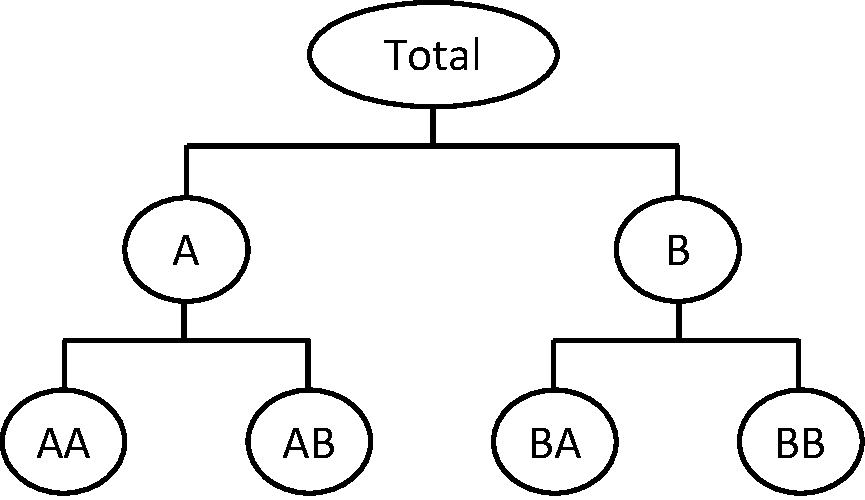
\includegraphics[width=0.3\textwidth,height=\textheight]{figs/hts_example.pdf}

}

\caption{\label{fig-hts}An example of a two-level hierarchical time
series.}

\end{figure}%

For example, Figure~\ref{fig-hts} shows a simple hierarchy with
\(n = 7\), \(n_b = 4\), \(n_a = 3\),
\(\bm{y}_t = [y_{\text{Total},t}, y_{\text{A},t}, y_{\text{B},t}, y_{\text{AA},t}, y_{\text{AB},t}, y_{\text{BA},t}, y_{\text{BB},t}]^{\prime}\),
\(\bm{b}_t = [y_{\text{AA},t}, y_{\text{AB},t}, y_{\text{BA},t}, y_{\text{BB},t}]^{\prime}\),
and \[
\bm{S} = \left[
\begin{array}{cccc}
1 & 1 & 1 & 1 \\
1 & 1 & 0 & 0 \\
0 & 0 & 1 & 1 \\
\multicolumn{4}{c}{\bm{I}_4}
\end{array}\right].
\] The notation is general enough to include aggregation constraints
that are non-hierarchical. Please refer to \citet{Hyndman2021-fo} for
further details.

Hierarchical forecasting methods have been extensively applied across
diverse domains. For instance, forecast reconciliation is widely
implemented in tourism data \citep{Athanasopoulos2009-ps}, where
hierarchical time series arise due to geographic divisions. Total
overnight trips for a whole nation can be disaggregated to states, and
further subdivided into regions. In the context of a grocery retailer,
the total sales of the ``food'' category can be subdivided into various
subcategories and subsequently into distinct items
\citep{Zhang2023-op, Hollyman2021-un}. In electricity load forecasting,
consumption is measured using smart meters which naturally fall within a
comprehensive geographic hierarchy \citep{Taieb2021-tc}. For additional
interesting application examples, please refer to
\citet{Athanasopoulos2024-sm}.

\subsection{Linear forecast
reconciliation}\label{linear-forecast-reconciliation}

Let \(\hat{\bm{y}}_{T+h \mid T} \in \mathbb{R}^n\) be a vector of
\(h\)-step-ahead \emph{base forecasts} for all time series in the
hierarchy, given observations up to and including time \(T\), and
stacked in the same order as \(\bm{y}_t\). We can use any method to
generate these forecasts, but in general they will not be coherent
(i.e., they won't satisfy the aggregation constraints). Let
\(\tilde{\bm{y}}_{T+h \mid T} \in \mathbb{R}^n\) denote a vector of
\(h\)-step-ahead \emph{reconciled forecasts} given by
\begin{equation}\phantomsection\label{eq-lr}{
\tilde{\bm{y}}_{T+h \mid T} = \bm{S}\bm{G}_h\hat{\bm{y}}_{T+h \mid T},
}\end{equation} where \(\bm{G}_h\) is an \(n_b \times n\)
\emph{weighting matrix}.

In general, forecast reconciliation methods consider the loss function
\citep{Ben_Taieb2019-be} given by
\begin{equation}\phantomsection\label{eq-loss}{
\begin{aligned}
& \mathrm{E}\left[\left\|\bm{y}_{T+h}-\tilde{\bm{y}}_{T+h \mid T}\right\|_2^2 \mid \bm{I}_T\right] \\
& =\underbrace{\left\|\bm{S G_h}\left(\mathrm{E}\left[\hat{\bm{y}}_{T+h \mid T} \mid \bm{I}_T\right]-\mathrm{E}\left[\bm{y}_{T+h} \mid \bm{I}_T\right]\right)+(\bm{S}-\bm{S G_h S}) \mathrm{E}\left[\bm{b}_{T+h} \mid \bm{I}_T\right]\right\|_2^2}_{\text{bias}} +\underbrace{\operatorname{Tr}\left(\operatorname{Var}\left[\bm{y}_{T+h}-\tilde{\bm{y}}_{T+h \mid T} \mid \bm{I}_T\right]\right)}_{\text{variance}},
\end{aligned}
}\end{equation} which includes two parts in its decomposition, bias and
variance of the reconciled forecasts.

\subsubsection*{Minimum trace
reconciliation}\label{minimum-trace-reconciliation}
\addcontentsline{toc}{subsubsection}{Minimum trace reconciliation}

Let
\(\hat{\bm{e}}_{t+h \mid t} = \bm{y}_{t+h} - \hat{\bm{y}}_{t+h \mid t}\)
denote the \(h\)-step-ahead in-sample \emph{base forecast errors}, and
\(\tilde{\bm{e}}_{t+h \mid t} = \bm{y}_{t+h} - \tilde{\bm{y}}_{t+h \mid t}\)
denote the \(h\)-step-ahead \emph{reconciled forecast errors}. Assuming
the base forecasts are unbiased and imposing the constraint
\(\bm{G}_h\bm{ S}=\bm{I}_{n_b}\) to preserve the unbiasedness of the
reconciled forecasts, the bias term in Equation \eqref{eq-loss} cancels.
\citet{Wickramasuriya2019-fc} thus formulated the reconciliation problem
as minimizing the trace (MinT) of the \(h\)-step-ahead covariance matrix
of the reconciled forecast errors, leading to the unique solution given
by \begin{equation}\phantomsection\label{eq-mint}{
\bm{G}_h=\left(\bm{S}^{\prime} \bm{W}_h^{-1} \bm{S}\right)^{-1} \bm{S}^{\prime} \bm{W}_h^{-1},
}\end{equation} where \(\bm{W}_h\) is the positive definite covariance
matrix of the \(h\)-step-ahead base forecast errors.

The MinT problem can be reformulated as a least squares problem with
linear constraints: \begin{equation}\phantomsection\label{eq-mint_op}{
\min_{\tilde{\bm{y}}_{T+h \mid T}} \quad \frac{1}{2}(\hat{\bm{y}}_{T+h \mid T}-\tilde{\bm{y}}_{T+h \mid T})^{\prime} \bm{W}_{h}^{-1}(\hat{\bm{y}}_{T+h \mid T}-\tilde{\bm{y}}_{T+h \mid T})
 \qquad \text{s.t.} \quad \tilde{\bm{y}}_{T+h \mid T}=\bm{S}\tilde{\bm{b}}_{T+h \mid T},
}\end{equation} where
\(\tilde{\bm{b}}_{T+h \mid T} \in \mathbb{R}^{n_b}\) comprises the
\(h\)-step-ahead bottom-level reconciled forecasts, made at time \(T\).
The intuition behind MinT reconciliation is that the larger the
estimated variance of the base forecast errors, the larger the range of
adjustments permitted for forecast reconciliation.

It is challenging to estimate \(\bm{W}_h\), especially for \(h > 1\). It
is common to assume \(\bm{W}_h = k_h\bm{W}_1\), \(\forall h\), where
\(k_h > 0\); then the MinT solution for \(\bm{G}\) remains unchanged
across different forecast horizons, \(h\). Hence, we will drop the
subscript \(h\) for ease of exposition. Table~\ref{tbl-bench} lists the
most popularly used candidate estimators for \(\bm{W}_h\). In principle,
all optimization methods can be based on either in-sample or
out-of-sample data. The methods discussed here are considered
``out-of-sample'' as they use genuine forecasts,
\(\hat{\bm{y}}_{T+h \mid T}\), rather than ``in-sample'' fitted values
for the optimization process.

\begin{table}

\caption{\label{tbl-bench}Forecast reconciliation methods for which
different estimators of \(\bm{W}_h\) are used.}

\centering{

\centering
\begin{threeparttable}
\begin{tabular}{p{0.5\linewidth}r}
\toprule
Reconciliation method & $\bm{W}_h\propto$\\
\midrule
\textbf{OLS} \citep{Hyndman2011-sd} & $\bm{I}$\\
\textbf{WLSs} \citep{Athanasopoulos2017-jj} & $\operatorname{diag}(\bm{S} \bm{1})$\\
\textbf{WLSv} \citep{Hyndman2016-cz} & $\operatorname{Diag}(\hat{\bm{W}}_1)$\\
\textbf{MinT} \citep{Wickramasuriya2019-fc} & $\hat{\bm{W}}_1$\\
\textbf{MinTs} \citep{Wickramasuriya2019-fc} & $\lambda\operatorname{Diag}(\hat{\bm{W}}_1) + (1-\lambda)\hat{\bm{W}}_1$\\
\bottomrule
\end{tabular}
\begin{tablenotes}[para]
\item \footnotesize{Note: $\bm{1}$ is a vector of 1s of size $n_b$, $\operatorname{diag}(\cdot)$ constructs a diagonal matrix using a given vector, $\hat{\bm{W}}_1$ denotes the unbiased covariance estimator based on the in-sample one-step-ahead base forecast errors (i.e., residuals), and $\operatorname{Diag}(\cdot)$ forms a diagonal matrix using the diagonal elements of the input matrix.}
\end{tablenotes}
\end{threeparttable}

}

\end{table}%

\subsubsection*{Relaxation of the unbiasedness
assumptions}\label{relaxation-of-the-unbiasedness-assumptions}
\addcontentsline{toc}{subsubsection}{Relaxation of the unbiasedness
assumptions}

\citet{Ben_Taieb2019-be} proposed a reconciliation method relaxing the
assumption of unbiasedness. Their goal was to achieve a tradeoff between
bias and variance by directly minimizing the mean squared reconciled
forecast errors in Equation \eqref{eq-loss}. By expanding the training
window incrementally, one observation at a time, they formulated the
reconciliation problem as a regularized empirical risk minimization
(RERM) problem: \[
\min_{\bm{G}_h} \frac{1}{(T-T_1-h+1)n}\left\|\bm{Y}_{h}^{*}-\hat{\bm{Y}}_{h}^{*} \bm{G}_{h}^{\prime} \bm{S}^{\prime}\right\|_F^2+\lambda\|\operatorname{vec}( \bm{G}_h)\|_1,
\] where \(T_1\) denotes the minimum number of observations used for
model training, \(\left\| \cdot \right\|_F\) is the Frobenius norm,
\(\|\cdot\|_1\) is the \(L_1\) norm, \(\operatorname{vec}(\cdot)\)
denotes the vectorization of a matrix (stacking the columns of the
matrix),
\(\bm{Y}_{h}^{*}=\left[\bm{y}_{T_1+h}, \ldots, \bm{y}_T\right]^{\prime}\),
\(\hat{\bm{Y}}_{h}^{*}=\left[\hat{\bm{y}}_{T_1+h \mid T_1}, \ldots, \hat{\bm{y}}_{T \mid T-h}\right]^{\prime}\),
and \(\lambda \geq 0\) is a regularization parameter.

When \(\lambda = 0\), the problem reduces to an empirical risk
minimization (ERM) problem without regularization. Assuming that the
series in the structure are jointly weakly stationary and
\(\hat{\bm{Y}}_{h}^{*\prime}\hat{\bm{Y}}_{h}^{*}\) is invertible, it has
a closed-form solution given by \[
\hat{\bm{G}}_h = \bm{B}_{h}^{*\prime}\hat{\bm{Y}}_{h}^{*}\left(\hat{\bm{Y}}_{h}^{*\prime}\hat{\bm{Y}}_{h}^{*}\right)^{-1},
\] where
\(\bm{B}_{h}^{*}=\left[\bm{b}_{T_1+h}, \ldots, \bm{b}_T\right]^{\prime}\).
If \(\hat{\bm{Y}}_{h}^{*\prime}\hat{\bm{Y}}_{h}^{*}\) is not invertible,
a generalized inverse can be applied. When \(\lambda > 0\), imposing the
\(L_1\) penalty on \(\bm{G}_h\) will introduce sparsity and reduce
estimation variance, albeit at the cost of introducing some bias.

Relaxing the assumption of unbiasedness of base forecasts,
\citet{Wickramasuriya2021-am} proposed an empirical MinT
(\textbf{EMinT}) solution by minimizing the trace of the covariance
matrix of the reconciled forecast errors. Assuming the series are
jointly weakly stationary, the solution is given by \[
\hat{\bm{G}}_{h} = \bm{B}_{h}^{\prime}\hat{\bm{Y}}_{h}\left(\hat{\bm{Y}}_{h}^{\prime}\hat{\bm{Y}}_{h}\right)^{-1},
\] where
\(\bm{B}_{h}=\left[\bm{b}_{h}, \ldots, \bm{b}_T\right]^{\prime}\), and
\(\hat{\bm{Y}}_{h}=\left[\hat{\bm{y}}_{h \mid 0}, \ldots, \hat{\bm{y}}_{T \mid T-h}\right]^{\prime}\).

The difference between EMinT and ERM lies in the data sources. EMinT is
an ``in-sample'' method in the sense that \(\hat{\bm{Y}}_{h}\) are
predictions in the form of fitted values, while ERM (and also RERM) is
an ``out-of-sample'' method, with \(\hat{\bm{Y}}_{h}^{*}\) being genuine
forecasts generated on a holdout validation set. Both EMinT and ERM
consider an estimate of \(\bm{G}\) that changes over the forecast
horizon, which is why we keep the subscript \(h\) here.

In practical settings, some series in a hierarchy could have poor base
forecasts due to model misspecification or low forecastability.
Specifically, within a hierarchical structure, the influence of
unforeseen events may prompt a forecaster to make a bad decision,
leading to the use of a misspecified forecasting model for a specific
time series and, consequently, yielding inferior forecasts. Moreover,
lower-level time series are normally characterized by less apparent
trend and seasonality, large intermittence, and volatility, rendering
them more challenging to predict and resulting in poor forecasts.

A challenge in forecast reconciliation arises when some base forecasts
perform poorly, as the weighting matrix \(\bm{G}\) assimilates
\emph{all} base forecasts and maps them into bottom-level forecasts,
which are subsequently summed by \(\bm{S}\). While the RERM method
introduces sparsity by shrinking some elements of \(\bm{G}\) towards
zero, it remains incapable of mitigating the adverse impact of
underperforming base forecasts. Moreover, the method is time-consuming
because it uses expanding windows to recursively generate out-of-sample
base forecasts.

In addition to \citet{Ben_Taieb2019-be}, several other contributions
have incorporated diverse forms of shrinkage or penalization in forecast
reconciliation methodologies. For example, \citet{Pang2022-hi}
introduced a group Lasso penalty on weights assigned to clusters
artificially added in a hierarchy to select ideal clusters. Their
objective function focuses on a new hierarchical structure encompassing
geographic and data cluster hierarchies, while disregarding forecast
errors associated with zero-weighted clusters. Furthermore, they derive
the optimal weight vector and optimal bottom level forecasts by solving
the objective successively, leading to a time-consuming method that does
not permanently mitigate the negative impact of poorly performing
clusters on reconciliation performance. To address the insufficient
emphasis on coherence in machine learning methods,
\citet{Mishchenko2019-as} and \citet{Gleason2020-fo} included a
regularization term to penalize forecast incoherence. However, these
soft constraints do not ensure coherence. \citet{Nystrup2020-te} and
\citet{Nystrup2021-di} considered the autocorrelation in forecast errors
and used a shrinkage estimator or eigendecomposition of the
cross-correlation matrix, effectively overcoming estimation
inefficiencies in approximating \(\bm{W}\) within a temporal hierarchy.
Nonetheless, none of the aforementioned contributions achieve time
series selection in forecast reconciliation, failing to alleviate their
adverse impact on forecast performance, while maintaining consideration
for forecast errors across the entire initial hierarchy.

We therefore propose two types of forecast reconciliation methods
involving time series selection: constrained ``out-of-sample''
reconciliation and unconstrained ``in-sample'' reconciliation. These
methods aim to address the negative effect of some poor base forecasts
on the overall performance of the reconciled forecasts. Additionally,
through the incorporation of regularization in the objective function,
our method improves reconciliation outcomes produced with a ``poor''
choice of \(\bm{W}\).

\section{Forecast reconciliation with time series
selection}\label{sec-methodology}

In this section, we introduce our methods for forecast reconciliation
while automatically achieving time series selection.
Section~\ref{sec-constrained} introduces constrained ``out-of-sample''
reconciliation methods, formulated based on genuine forecasts, while
Section~\ref{sec-unconstrained} presents an unconstrained ``in-sample''
reconciliation method, where the problem is formulated using in-sample
observations and predictions in the form of fitted values.

\subsection{Series selection under the unbiasedness
assumption}\label{sec-constrained}

As \(\bm{S}\) is fixed and \(\hat{\bm{y}}_{T+h \mid T}\) is given,
\(\bm{G}_h\) determines the linear reconciliation performance, as shown
in Equation \eqref{eq-lr}. We drop the subscript \(h\) here as we assume
\(\bm{W}\) and \(\bm{G}\) do not vary with the forecast horizon. A
natural way to remove forecasts of some series is by controlling the
number of nonzero column entries in \(\bm{G}\). This leads to a
generalization of the MinT optimization problem with an additional
penalty term: \begin{equation}\phantomsection\label{eq-op_u}{
\min_{\bm{G}} \quad \frac{1}{2}\left(\hat{\bm{y}}-\bm{SG}\hat{\bm{y}}\right)^{\prime} \bm{W}^{-1}\left(\hat{\bm{y}}-\bm{SG}\hat{\bm{y}}\right)
+ \lambda\mathfrak{g}(\bm{G}) \qquad \text{s.t.} \quad \bm{G}\bm{S}=\bm{I},
}\end{equation} where \(\hat{\bm{y}}:=\hat{\bm{y}}_{T+1 \mid T}\),
\(\mathfrak{g}(\cdot)\) penalizes the columns of \(\bm{G}\) towards
zero, and \(\lambda\) is a penalty parameter. The methods developed
within this framework are ``out‑of‑sample'' in the sense that
\(\hat{\bm{y}}\) are genuine one-step-ahead forecasts. This can be
considered \emph{a grouped variable selection problem}, with each group
corresponding to a column of \(\bm{G}\). When \(\lambda = 0\), the
problem reduces to the MinT optimization problem in Equation
\eqref{eq-mint_op} with a closed-form solution given by Equation
\eqref{eq-mint}.

The constraint \(\bm{G}\bm{S}=\bm{I}\) guarantees that the reconciled
forecasts remain unbiased if the base forecasts are unbiased. Under this
assumption and constraint, minimizing the loss function in Equation
\eqref{eq-loss} simplifies to the MinT problem formulated in Equation
\eqref{eq-mint_op}, which underpins the constrained ``out-of-sample''
reconciliation methods within the framework in equation \eqref{eq-op_u}.

\begin{proposition}[]\protect\hypertarget{prp-1}{}\label{prp-1}

If the assumption that forecast reconciliation preserves unbiasedness is
imposed by enforcing \(\bm{GS}=\bm{I}\), then the number of nonzero
column entries of \(\hat{\bm{G}}\) (the solution to Equation
\eqref{eq-op_u}) will be no less than \(n_b\). Moreover, the constraint
\(\bm{GS}=\bm{I}\) enforces that the selected columns of
\(\hat{\bm{G}}\) will correspond to variables that can ``restore'' the
hierarchy.

\end{proposition}

\begin{proof}
See \hyperref[appendix-proofs]{Appendix A}, supplementary materials.
\end{proof}

For example, for the simple hierarchy shown in Figure~\ref{fig-hts}, the
selected columns of \(\hat{\bm{G}}\) will be at least \(n_b=4\). Our
constrained reconciliation methods might simultaneously zero out the
columns of \(\bm{G}\) corresponding to series AA and BA, but not to
series AA and AB.

\begin{proposition}[]\protect\hypertarget{prp-2}{}\label{prp-2}

The optimization problem in Equation \eqref{eq-op_u} can be reformulated
as a least squares problem with regularization and linear equality
constraint as follows:
\begin{equation}\phantomsection\label{eq-op_u_reg}{
\begin{aligned}
& \min_{\operatorname{vec}(\bm{G})} \quad \frac{1}{2}\left(\hat{\bm{y}}-\left(\hat{\bm{y}}^{\prime} \otimes \bm{S}\right) \operatorname{vec}(\bm{G})\right)^{\prime} \bm{W}^{-1}\left(\hat{\bm{y}}-\left(\hat{\bm{y}}^{\prime} \otimes \bm{S}\right) \operatorname{vec}(\bm{G})\right) + \lambda\mathfrak{g}\left(\operatorname{vec}(\bm{G})\right) \\
& \text{s.t.} \quad \left(\bm{S}^{\prime} \otimes \bm{I}_{n_b}\right) \operatorname{vec}(\bm{G})=\operatorname{vec}(\bm{I}_{n_b}),
\end{aligned}
}\end{equation} which is characterized as a high-dimensional problem in
which the number of features, denoted as \(p = n_b \times n\), is much
larger than the number of observations, \(n\).

\end{proposition}

\begin{proof}
See \hyperref[appendix-proofs]{Appendix A}, supplementary materials.
\end{proof}

Next, we present three constrained ``out-of-sample'' reconciliation
methods: (i) group best-subset selection with ridge regularization, (ii)
parsimonious method with \(L_0\) regularization, and (iii) group lasso
method. These methods perform forecast reconciliation with series
selection under the unbiasedness assumption, differing only in the
regularization term employed.

\subsubsection*{Group best-subset selection with ridge
regularization}\label{group-best-subset-selection-with-ridge-regularization}
\addcontentsline{toc}{subsubsection}{Group best-subset selection with
ridge regularization}

In a high-dimensional context with \(p \gg n\), it is common to assume
that the true regression coefficient (i.e.,
\(\operatorname{vec}(\bm{G})\) in our problem) is sparse. We apply a
combination of \(L_0\) and \(L_2\) regularization to control the nonzero
column entries in \(\bm{G}\):
\begin{equation}\phantomsection\label{eq-subset}{ \begin{aligned}
\min_{\operatorname{vec}(\bm{G})} \quad & \frac{1}{2}\left(\hat{\bm{y}}-\left(\hat{\bm{y}}^{\prime} \otimes \bm{S}\right) \operatorname{vec}(\bm{G})\right)^{\prime} \bm{W}^{-1}\left(\hat{\bm{y}}-\left(\hat{\bm{y}}^{\prime} \otimes \bm{S}\right) \operatorname{vec}(\bm{G})\right) + \lambda_0 \sum_{j=1}^n 1\left(\bm{G}_{\cdot j} \neq \bm{0}\right) + \lambda_2 \left\|\operatorname{vec}\left(\bm{G}\right)\right\|_2^2 \\
\text{s.t.} \quad & \left(\bm{S}^{\prime} \otimes \bm{I}_{n_b}\right) \operatorname{vec}(\bm{G})=\operatorname{vec}(\bm{I}_{n_b}),
\end{aligned}
}\end{equation} where \(1(\cdot)\) is the indicator function,
\(\lambda_0 \geq 0\) controls the number of nonzero columns of
\(\bm{G}\), \(\lambda_2 \geq 0\) controls the strength of the ridge
regularization, and \(\|\cdot\|_2\) is the \(L_2\) norm. In a
hierarchical or grouped time series context,
\(\operatorname{vec}(\bm{G})\) has an inherent non-overlapping grouping
structure, wherein each group corresponds to a single column of
\(\bm{G}\), each of size \(n_b\). Hence, we call this reconciliation
method \emph{group best-subset selection with ridge regularization}. In
the results that follow, we label the \textbf{Subset} method differently
based on various \(\bm{W}\) estimators, referring to them as
\textbf{OLS-subset}, \textbf{WLSs-subset}, \textbf{WLSv-subset},
\textbf{MinT-subset}, and \textbf{MinTs-subset}, respectively.

The best-subsets estimator, derived from an \(L_0\)-regularized least
squares problem, is a natural and direct candidate for sparse learning.
The \(L_0\) penalty leads to models that have a subset of coefficients
exactly equal to zero, effectively performing variable selection. The
statistical properties of the best-subsets estimator have been
extensively studied; see, for example, \citet{Greenshtein2004-be},
\citet{Zhang2012-ge}, and the references therein. However,
\citet{Mazumder2022-hx} argued that the vanilla \(L_0\) penalization
could suffer from overfitting in low SNR settings. To address the issue,
we incorporate a ridge regularization in Equation \eqref{eq-subset},
motivated by earlier work on best-subset selection
\citep[e.g.,][]{Hazimeh2020-xd, Mazumder2022-hx}, which suggests that
additional ridge regularization helps mitigate the poor predictive
performance of best-subset selection method in low SNR regimes.

We present a Big-M based mixed integer programming (MIP) formulation for
the problem in Equation \eqref{eq-subset}:
\begin{equation}\phantomsection\label{eq-subset_mip}{
\begin{aligned}
\min_{\operatorname{vec}(\bm{G}), \bm{z}, \check{\bm{e}}, \bm{g}^{+}} & \frac{1}{2}\check{\bm{e}}^{\prime} \bm{W}^{-1}\check{\bm{e}} + \lambda_0 \sum_{j=1}^n z_j + \lambda_2 \bm{g}^{+\prime}\bm{g}^{+} \\
\text{s.t.} \quad & \left(\bm{S}^{\prime} \otimes \bm{I}_{n_b}\right) \operatorname{vec}(\bm{G})=\operatorname{vec}\left(\bm{I}_{n_b}\right) \\
& \hat{\bm{y}}-\left(\hat{\bm{y}}^{\prime} \otimes \bm{S}\right)\operatorname{vec}(\bm{G}) = \check{\bm{e}} \\
& \sum_{i=1}^{n_b} g_{i + (j-1) n_b}^{+} \leqslant \mathcal{M} z_j, \quad j \in[n] \\
& \bm{g}^{+} \geqslant \operatorname{vec}(\bm{G}) \\
& \bm{g}^{+} \geqslant-\operatorname{vec}(\bm{G}) \\
& z_j \in\{0,1\}, \quad j \in[n],
\end{aligned}
}\end{equation} where \(\mathcal{M}\) is a Big-M parameter (specified
a-priori) that is sufficiently large that the optimal solution to
Equation \eqref{eq-subset_mip}, \(\bm{g}^{+*}\), satisfies
\(\max_{j \in [n]}\sum_{i=1}^{n_b} g_{i + (j-1) n_b}^{+} \leqslant \mathcal{M}\).
The binary variable \(z_j=0\) implies that \(\bm{G}_{\cdot j}=\bm{0}\),
and \(z_j=1\) implies that
\(\sum_{i=1}^{n_b} g_{i + (j-1) n_b}^{+} \leqslant \mathcal{M}\). Such
Big-M formulations are commonly used in MIP problems to model relations
between discrete and continuous variables, and have been recently
explored in regression with \(L_0\) regularization
\citep{Bertsimas2016-ig}. The problem is a mixed integer quadratic
program (MIQP) that can be solved using commercial MIP solvers, e.g.,
Gurobi and CPLEX.

\textbf{Parameter tuning.} To avoid computationally expensive
cross-validation, we tune the parameters to minimize the sum of squared
reconciled forecast errors on the truncated training set, comprising
only the \(\max\{h, s\}\) observations closest to the forecast origin,
where \(s\) is the seasonal period for seasonal data and \(s=T\) for
non-seasonal data. Let
\(\lambda_{0}^{1} = \frac{1}{2}\left(\hat{\bm{y}}-\tilde{\bm{y}}^{\text{bench}}\right)^{\prime} \bm{W}^{-1}\left(\hat{\bm{y}}-\tilde{\bm{y}}^{\text{bench}}\right)\),
which captures the scale of the first term in the objective function,
where \(\tilde{\bm{y}}^{\text{bench}}\) is a vector of reconciled
forecasts obtained using Equation \eqref{eq-mint} with the same
estimator of \(\bm{W}\), and define
\(\lambda_{0}^{k} = 0.0001\lambda_{0}^{1}\). For the parameter
\(\lambda_0\), we consider a grid of \(k+1\) values,
\(\{\lambda_{0}^{1},\dots,\lambda_{0}^{k}, 0\}\), where
\(\lambda_{0}^{j} = \lambda_{0}^{1}\left(\lambda_{0}^{k} / \lambda_{0}^{1}\right)^{(j-1) / (k-1)}\)
for \(j \in [k]\). So \(\lambda_{0}^{1},\dots,\lambda_{0}^{k}\) is a
sequence decreasing on the log scale. We use a grid of six values for
the parameter \(\lambda_2\),
\(\{0, 10^{-2}, 10^{-1}, 10^{0}, 10^{1}, 10^{2}\}\). Thus, we tune over
a two-dimensional grid of \((k+1) \times 6\) values to find the optimal
combination of \(\lambda_0\) and \(\lambda_2\).

\textbf{Computation details.} The MIQP problem in Equation
\eqref{eq-subset_mip} is NP-hard and computationally intensive.
\citet{Bertsimas2016-ig} showed that commercial MIP solvers are capable
of tackling problem instances for \(p\) up to a thousand. To address
larger instances, there has been impressive work on developing MIP-based
approaches for solving \(L_0\)-regularized regression problem; e.g.,
\citet{Bertsimas2016-ig}, \citet{Hazimeh2020-xd}, and
\citet{Hazimeh2022-hc}. However, it is challenging to extend these
approaches to accommodate additional constraints in the optimization
problem. Despite potential challenges in handling large instances with
commercial MIP solvers, in our experiments, we use Gurobi to solve
Equation \eqref{eq-subset_mip} by configuring parameters such as MIPGap
= \(0.001\) and TimeLimit = \(600\) seconds for cases with \(p > 1000\).
This allows to terminate the solver before reaching the global optimum
and return a suboptimal solution instead. This strategy is motivated by
our need to consider numerous parameter candidates, and the final
solution will be validated against the training set, which prevents the
use of a poor estimate of \(\bm{G}\).

\subsubsection*{\texorpdfstring{Parsimonious method with \(L_0\)
regularization}{Parsimonious method with L\_0 regularization}}\label{parsimonious-method-with-l_0-regularization}
\addcontentsline{toc}{subsubsection}{Parsimonious method with \(L_0\)
regularization}

Instead of estimating the entire matrix \(\bm{G}\) as above, we leverage
the MinT solution in Equation \eqref{eq-mint} to streamline the
optimization problem under consideration. Specifically, we define
\(\bar{\bm{S}} = \bm{A}\bm{S}\), where
\(\bm{A} = \operatorname{diag}(\bm{z})\) is an \(n \times n\) diagonal
matrix, and \(\bm{z}\) is an \(n\)-dimensional vector with elements
either equal to 0 or 1. Taking the MinT solution in Equation
\eqref{eq-mint}, we have
\(\bar{\bm{G}} = (\bm{S}^{\prime}\bm{A}^{\prime}\bm{W}^{-1}\bm{A}\bm{S})^{-1}\bm{S}^{\prime}\bm{A}^{\prime}\bm{W}^{-1}\).
Given fixed \(\bm{S}\) and estimation of \(\bm{W}\), \(\bar{\bm{G}}\) is
entirely determined by \(\bm{A}\). Thus, when the \(j\)th diagonal
element of \(\bm{A}\) is zero, the \(j\)th column of \(\bar{\bm{G}}\)
becomes entirely composed of zeros. Therefore, the optimization problem
can be reduced to an integer quadratic programming problem where all of
the variables are restricted to being integers: \begin{align*}
\min_{\bm{A}} \quad & \frac{1}{2}\left(\hat{\bm{y}}-\bm{S}\bar{\bm{G}}\hat{\bm{y}}\right)^{\prime} \bm{W}^{-1}\left(\hat{\bm{y}}-\bm{S}\bar{\bm{G}}\hat{\bm{y}}\right) + \lambda_0 \sum_{j=1}^n \bm{A}_{jj} \\
\text{s.t.} \quad & \bar{\bm{G}} = (\bm{S}^{\prime}\bm{A}^{\prime}\bm{W}^{-1}\bm{A}\bm{S})^{-1}\bm{S}^{\prime}\bm{A}^{\prime}\bm{W}^{-1} \qquad\text{and}\qquad \bar{\bm{G}}\bm{S} = \bm{I},
\end{align*} where \(\lambda_0 \geq 0\) controls the number of nonzero
diagonal elements in \(\bm{A}\), consequently affecting the number of
nonzero columns (i.e., selected time series) in \(\bm{G}\). We call this
reconciliation method the \emph{parsimonious method with} \(L_0\)
\emph{regularization} due to its appeal in reducing the number of
parameters. In the results that follow, we label the
\textbf{Parsimonious} method differently based on various estimators for
\(\bm{W}\), referring to them as \textbf{OLS-parsim},
\textbf{WLSs-parsim}, \textbf{WLSv-parsim}, \textbf{MinT-parsim}, and
\textbf{MinTs-parsim}, respectively.

In the Parsimonious method, the unknown matrix \(\bm{A}\) is restricted
to elements of \(0\) or \(1\). Thus the \(L_2\) penalty is excluded from
its optimization problem, unlike in the Subset method. We note that
achieving time series selection with this optimization problem can be
challenging, as identifying a solution \(\hat{\bm{A}}\) with some zero
diagonal elements while satisfying both the MinT solution and the
constraint may be difficult. Thus, the resulting solution tends to be
dense and may not have zero columns.

To ensure the invertibility of
\(\bm{S}^{\prime}\bm{A}^{\prime}\bm{W}^{-1}\bm{A}\bm{S}\), and make the
problem compatible with Gurobi, we reformulate the problem as
\begin{equation}\phantomsection\label{eq-parsimonious_mip}{
\begin{aligned}
\min_{\bm{A},\bar{\bm{G}},\bm{C},\check{\bm{e}},\bm{z}} \quad & \frac{1}{2}\check{\bm{e}}^{\prime} \bm{W}^{-1}\check{\bm{e}} + \lambda_0 \sum_{j=1}^n z_j \\
\text{s.t.} \quad & \bar{\bm{G}}\bm{S} = \bm{I} \\
& \hat{\bm{y}}-\left(\hat{\bm{y}}^{\prime} \otimes \bm{S}\right)\operatorname{vec}(\bar{\bm{G}}) = \check{\bm{e}} \\
& \bar{\bm{G}}\bm{A}\bm{S} = \bm{I} \\
& \bar{\bm{G}} = \bm{C}\bm{S}^{\prime}\bm{A}^{\prime}\bm{W}^{-1} \\
& z_j \in\{0,1\}, \quad j \in[n].
\end{aligned}
}\end{equation}

\textbf{Parameter tuning.} Similar to the setup in the group best-subset
selection, we select the tuning parameter, \(\lambda_0\), by minimizing
the sum of squared reconciled forecast errors on a truncated training
set, comprising only the \(\max\{h, s\}\) observations that occurred
prior to the forecast origin. Let
\(\lambda_{0}^{1} = \frac{1}{2}\left(\hat{\bm{y}}-\tilde{\bm{y}}^{\text{bench}}\right)^{\prime} \bm{W}^{-1}\left(\hat{\bm{y}}-\tilde{\bm{y}}^{\text{bench}}\right)\),
and \(\lambda_{0}^{k} = 0.0001\lambda_{0}^{1}\), the collection of
candidate values for \(\lambda_0\) we consider is
\(\{\lambda_{0}^{1},\dots,\lambda_{0}^{k}, 0\}\), where
\(\lambda_{0}^{j} = \lambda_{0}^{1}\left(\lambda_{0}^{k} / \lambda_{0}^{1}\right)^{(j-1) / (k-1)}\)
for \(j \in [k]\).

\textbf{Computation details.} Following a setup akin to that in the
group best-subset selection, we employ Gurobi to solve Equation
\eqref{eq-parsimonious_mip} by configuring parameters such as MIPGap =
\(0.001\) and TimeLimit = \(600\) seconds for problems with
\(p > 1000\).

\subsubsection*{Group lasso method}\label{group-lasso-method}
\addcontentsline{toc}{subsubsection}{Group lasso method}

\citet{Yuan2006-mw} introduced the group lasso method, which extends
lasso to situations with a grouped structure among variables. Similar to
lasso, group lasso induces sparsity, but at the group level, leading to
more interpretable models by reducing the number of non-zero groups of
coefficients. \citet{Lounici2011-or} demonstrated that group lasso
enhances prediction and estimation properties compared to the
traditional lasso method. The statistical properties of the group-lasso
estimator have been extensively studied in the literature
\citep[e.g.,][]{Nardi2008-asymptotic}.

When the problem of forecast reconciliation with time series selection
is reframed as a least squares problem, our goal is to perform
group-wise variable selection. Specifically, the unknown paramter
\(\operatorname{vec}(\bm{G})\) possesses an inherent grouping structure,
with each group corresponding to a single column of \(\bm{G}\), each of
size \(n_b\). Thus, we consider \emph{a group lasso problem under the
unbiasedness assumption} given by
\begin{equation}\phantomsection\label{eq-lasso}{
\begin{aligned}
\min_{\bm{G}} \quad & \frac{1}{2}\left(\hat{\bm{y}}-\left(\hat{\bm{y}}^{\prime} \otimes \bm{S}\right) \operatorname{vec}(\bm{G})\right)^{\prime} \bm{W}^{-1}\left(\hat{\bm{y}}-\left(\hat{\bm{y}}^{\prime} \otimes \bm{S}\right) \operatorname{vec}(\bm{G})\right) + \lambda \sum_{j=1}^n w_j \left\|\bm{G}_{\cdot j}\right\|_2 \\
\text{s.t.} \quad & \left(\bm{S}^{\prime} \otimes \bm{I}_{n_b}\right) \operatorname{vec}(\bm{G})=\operatorname{vec}\left(\bm{I}_{n_b}\right),
\end{aligned}
}\end{equation} where \(\lambda \geq 0\) is a tuning parameter,
\(w_j \neq 0\) is the penalty weight assigned in \(\bm{G}_{\cdot j}\) to
make the model more flexible, and the second term in the objective is
the penalty function that is intermediate between the \(L_1\)-penalty
that is used in the lasso and the \(L_2\)-penalty that is used in ridge
regression. In the results that follow, we label the \textbf{Lasso}
method based on various estimators for \(\bm{W}\), referring to them as
\textbf{OLS-lasso}, \textbf{WLSs-lasso}, \textbf{WLSv-lasso},
\textbf{MinT-lasso}, and \textbf{MinTs-lasso}, respectively.

Next, we present the second order cone programming (SOCP) formulation
for the group lasso based estimators given by
\begin{equation}\phantomsection\label{eq-lasso_socp}{
\begin{aligned}
\min_{\operatorname{vec}(\bm{G}), \check{\bm{e}}, \bm{g}^{+}} & \frac{1}{2}\check{\bm{e}}^{\prime} \bm{W}_h^{-1}\check{\bm{e}} + \lambda \sum_{j=1}^n w_j c_j \\
\text{s.t.} \quad & \left(\bm{S}^{\prime} \otimes \bm{I}_{n_b}\right) \operatorname{vec}(\bm{G})=\operatorname{vec}\left(\bm{I}_{n_b}\right) \\
& \hat{\bm{y}}-\left(\hat{\bm{y}}^{\prime} \otimes \bm{S}\right) \operatorname{vec}(\bm{G}) = \check{\bm{e}} \\
& c_j = \sqrt{\sum_{i=1}^{n_b} g_{i + (j-1) n_b}^{+2}}, \quad j \in[n].
\end{aligned}
}\end{equation} Equation \eqref{eq-lasso_socp} includes additional
auxiliary variables \(c_j \in \mathbb{R}_{\geq 0}\), \(j \in [n]\), and
second order cone constraints,
\(c_j = \sqrt{\sum_{i=1}^{n_b} g_{i + (j-1) n_b}^{+2}}\) for
\(j \in[n]\).

Compared to the previous two methods above, the group lasso method is
computationally friendlier. Nonetheless, \citet{Hazimeh2023-ie}
demonstrated, both empirically and theoretically, that the group
\(L_0\)-regularized method exhibits advantages over its group lasso
counterpart across a range of regimes. Group lasso can either be highly
dense or possess non-zero coefficients that are overly shrunk. This
issue becomes more pronounced when the groups are correlated with each
other, as group lasso tends to retain all correlated groups instead of
seeking a more concise model.

\textbf{Penalty weights and parameter tuning.} In the context of group
lasso, the default choice for the penalty weight, \(w_j\), is
\(\sqrt{p_j}\), where \(p_j\) is the size of each group (in our case,
\(p_j = n_b\)). In our experiments, we allocate different penalty
weights to each group using
\(w_j = 1/\|\bm{G}_{\cdot j}^{\text{bench}}\|_2\), which allows us to
account for variations in scale across different time series in the
structure.

We compute the group lasso over \(k+1\) values of the tuning parameter
\(\lambda\), and select the parameter by optimizing the sum of squared
reconciled forecast errors on a truncated training set, consisting only
of \(\max\{h, s\}\) observations occurred prior to the forecast origin.
The collection of candidate values for \(\lambda\) is
\(\{\lambda^{1},\dots,\lambda^{k}, 0\}\), where
\(\lambda^{1} = \max_{j=1, \ldots, n}\big\|-\big((\hat{\bm{y}}^{\prime} \otimes \bm{S})_{\cdot j^{*}}\big)^{\prime} \bm{W}^{-1} \hat{\bm{y}}\big\|_2 / w_j\),
\(\lambda^{k} = 0.0001\lambda^{1}\), and
\(\lambda^{j} = \lambda^{1}(\lambda^{k} / \lambda^{1})^{(j-1) / (k-1)}\)
for \(j \in [k]\).

\begin{proposition}[]\protect\hypertarget{prp-3}{}\label{prp-3}

Ignoring the constraint \(\bm{G_h S}=\bm{I_{n_b}}\), we define
\(\lambda^{1}\) as the smallest \(\lambda\) value such that all
predictors in the group lasso problem have zero coefficients. Then we
have \[
\lambda^{1} = \max_{j=1, \ldots, n}\big\|-\big((\hat{\bm{y}}^{\prime} \otimes \bm{S})_{\cdot j^{*}}\big)^{\prime} \bm{W}^{-1} \hat{\bm{y}}\big\|_2 / w_j,
\] where \(j^{*}\) denotes the column index of
\(\hat{\bm{y}}^{\prime} \otimes \bm{S}\) that corresponds to the \(j\)th
column of \(\bm{G}\).

\end{proposition}

\begin{proof}
See \hyperref[appendix-proofs]{Appendix A}, supplementary materials.
\end{proof}

\textbf{Computation details.} Due to the incorporation of the
constraint, we can not directly use some open-source packages designed
for group lasso. Consequently, we employ Gurobi to solve the SOCP
problem, configuring it by setting OptimalityTol = \(0.0001\).

\subsection{Series selection relaxing the unbiasedness
assumption}\label{sec-unconstrained}

In this section, we relax the unbiasedness assumption, and introduce a
reconciliation method with selection that relies on in-sample
observations and fitted values. Let
\(\bm{Y} \in \mathbb{R}^{T \times n}\) denote a matrix comprising
observations from all time series on the training set in the structure,
and \(\hat{\bm{Y}} \in \mathbb{R}^{T \times n}\) denote a matrix of
in-sample one-step-ahead forecasts (i.e., fitted values) for all time
series. The proposed \emph{empirical group lasso} method considers the
optimization problem \[
\min_{\bm{G}} \quad \frac{1}{2 T} \left\|\bm{Y}-\hat{\bm{Y}} \bm{G}^{\prime} \bm{S}^{\prime}\right\|_F^2 + \lambda \sum_{j=1}^n w_j \left\|\bm{G}_{\cdot j}\right\|_2,
\] where \(\lambda \geq 0\) is a tuning parameter, \(w_j \neq 0\) is the
penalty weight assigned in \(\bm{G}_{\cdot j}\) to make a more flexible
model. We rewrite the problem as \[
\min_{\operatorname{vec}(\bm{G})} \quad \frac{1}{2 T} \left\|\operatorname{vec}(\bm{Y})-(\bm{S} \otimes \hat{\bm{Y}}) \operatorname{vec}\left(\bm{G}^{\prime}\right)\right\|_2^2 + \lambda \sum_{j=1}^n w_j \left\|\bm{G}_{\cdot j}\right\|_2,
\] which becomes a standard group lasso problem, with
\(\operatorname{vec}(\bm{Y})\) serving as the dependent variable and
\(\bm{S} \otimes \hat{\bm{Y}}\) as the covariate matrix. We denote this
as \textbf{Elasso} in the results that follow.

Unlike the methods introduced in Section~\ref{sec-constrained}, Elasso
relaxes the unbiasedness conditions on both base and reconciled
forecasts and operates as an ``in-sample'' method because
\(\hat{\bm{Y}}\) are predictions in the form of fitted values (i.e.,
\(\bm{Y}\) is in training data when base forecasts are computed). Thus
Elasso aims to directly minimize the mean squared reconciled forecast
errors, as described in Equation \eqref{eq-loss}, rather than focusing
solely on the variance term. This clarifies two points: (1) why the
Elasso method omits the \(\bm{GS}=\bm{I}\) constraint, which ensures the
unbiasedness of reconciled forecasts when base forecasts are unbiased,
and (2) why the Elasso method does not use a \(\bm{W}\) matrix, which is
introduced when deriving from
\(\operatorname{Var}(\tilde{\bm{e}}_{T+h \mid T})\) under the
constraint.

We note that both the ``in-sample'' Elasso and EMinT methods require
only one round of model training. Similarly, the Subset, Parsimonious,
and Lasso methods also need only one round of training and forecasting,
despite their reliance on genuine out-of-sample forecasts. In contrast,
the ``out-of-sample'' RERM and ERM methods use an iterative approach
with expanding windows for out-of-sample forecasts, demanding extensive
rounds of model training and significant computation time. To ensure a
fair comparison, we exclude RERM and ERM methods from simulation studies
and empirical results.

Relaxing the unbiasedness assumption may result in fewer non-zero column
entries in the \(\bm{G}\) solution than the number of series at the
bottom level. This differs from constrained reconciliation methods
detailed in Section~\ref{sec-constrained}. In an extreme scenario, the
solution may take the form of a top-down
\(\bm{G}_{TD}=[\bm{p} \mid \bm{O}_{n_b \times (n-1)}]\), where only the
column corresponding to the top level (most aggregated level) retains
non-zero values, and \(\bm{p} = (p_1, p_2, \ldots, p_{n_b})\) is a
proportionality vector obtained based on in-sample reconciled forecast
errors.

We also explored the empirical version of group best-subset selection
with ridge regularization and the parsimonious method with \(L_0\)
regularization in which we omit the unbiasedness assumption. It is worth
mentioning that \citet{Hazimeh2023-ie} presented an algorithmic
framework for formulating the group \(L_0\) problem with ridge
regularization and provided the \textbf{L0Group} Python package for
implementation. However, our experiments showed that this algorithm can
not terminate within five hours for typical instances with
\(p \sim 10^4\). Therefore, in this paper, we only present the empirical
group lasso method for series selection without the unbiasedness
assumption.

\textbf{Penalty weights and parameter tuning.} Similar to the setup in
the group lasso method, we assign different penalty weights to each
group by setting \(w_j = 1/\|\bm{G}_{\cdot j}^{\text{OLS}}\|_2\), where
\(\bm{G}^{\text{OLS}}\) is the solution obtained by the OLS estimator of
\(\bm{W}\). Given a fixed tuning parameter, we solve the target
optimization problem by considering the initial \(T-T_v\) observations,
where \(T_v = \max\{h, s\}\) for seasonal time series and
\(T_v = \lfloor \frac{1}{10}T \rfloor\) for non-seasonal time series.
Then the tuning parameter, \(\lambda\), is selected by minimizing the
sum of squared reconciled forecast errors on a truncated training set,
comprising only the \(T_v\) observations closest to the forecast origin.
Specifically, for \(\lambda\) values, we consider
\(\{\lambda^{1},\dots,\lambda^{k}, 0\}\), where
\(\lambda^{1} = \max_{j=1, \ldots, n}\left\|-\frac{1}{N}\left(\left(\bm{S} \otimes \hat{\bm{Y}}\right)_{\cdot j*}\right)^{\prime} \operatorname{vec}(\bm{Y})\right\|_2 / w_j\),
\(\lambda^{k} = 0.0001\lambda^{1}\), and
\(\lambda^{j} = \lambda^{1}\left(\lambda^{k} / \lambda^{1}\right)^{(j-1) / (k-1)}\)
for \(j \in [k]\). Following the derivation in the proof of
Proposition~\ref{prp-3}, \(\lambda^{1}\) is the smallest \(\lambda\)
value such that all predictors in the empirical group lasso problem have
zero coefficients, i.e., \(\bm{G} = \bm{O}\). Note that we need to
resolve the optimization problem based on the whole training set by
using the optimal tuning parameter to obtain the final solution.

\textbf{Computation details.} While there are open-source packages
available for solving group lasso problems, they are still relatively
slow when handling large instances. For example, given a specific value
for the parameter, \(\lambda\), our experiments observed that, using the
\textbf{gglasso} R package, we can not obtain a solution within five
hours for typical instances with \(p \sim 10^4\). Instead, we use Gurobi
to solve the problem using the SOCP formulation for the empirical group
lasso which aligns with Equation \eqref{eq-lasso_socp} but omits the
constraint.

\section{Monte Carlo simulations}\label{sec-simulations}

To assess the proposed reconciliation methods with time series selection
outlined in Section~\ref{sec-methodology}, we carry out two simulations
with different designs. Both simulations consider a hierarchy comprising
two levels of aggregation, as shown in Figure~\ref{fig-hts}. The
bottom-level series are first generated and then summed to obtain the
aggregated series at higher levels.

\subsection{Setup 1: Exploring the effect of model
misspecification}\label{sec-sim1}

We follow a simulation setup similar to \citet{Wickramasuriya2019-fc},
assuming that the bottom-level time series are generated using the basic
structural time series model \[
\bm{b}_t=\bm{\mu}_t+\bm{\gamma}_t+\bm{\eta}_t,
\] where \(\bm{\mu}_t\) and \(\bm{\gamma}_t\) are trend and seasonal
components defined by \begin{align*}
\bm{\mu}_t & =\bm{\mu}_{t-1}+\bm{v}_t+\bm{\varrho}_t, &&& \bm{\varrho}_t & \sim \mathcal{N}\left(\bm{0}, \sigma_{\varrho}^2 \bm{I}_4\right), \\
\bm{v}_t & =\bm{v}_{t-1}+\bm{\zeta}_t, &&& \bm{\zeta}_t & \sim \mathcal{N}\left(\bm{0}, \sigma_\zeta^2 \bm{I}_4\right), \\
\bm{\gamma}_t & =-\sum_{i=1}^{s-1} \bm{\gamma}_{t-i}+\bm{\omega}_t, &&& \bm{\omega}_t & \sim \mathcal{N}\left(\bm{0}, \sigma_\omega^2 \bm{I}_4\right),
\end{align*} \(\bm{\varrho}_t\), \(\bm{\zeta}_t\), and \(\bm{\omega}_t\)
are error terms independent of each other and over time, and
\(\bm{\eta}_t\) is generated independently from an
\(\text{ARIMA}(p,0,q)\) process, where \(p\) and \(q\) take values of
\(0\) or \(1\) with equal probability. Coefficients in the ARIMA process
are randomly sampled from a uniform distribution \(U(0.5, 0.7)\), and
the contemporaneous error covariance matrix is given by \[
\left[\begin{array}{llll}
5 & 3 & 2 & 1 \\
3 & 4 & 2 & 1 \\
2 & 2 & 5 & 3 \\
1 & 1 & 3 & 4
\end{array}\right],
\] which enables correlations among time series in a hierarchical
structure.

We set \(s = 4\) for quarterly data with error variances
\(\sigma_{\varrho}^2=2\), \(\sigma_\zeta^2=0.007\), and
\(\sigma_\omega^2=7\). Initial values for \(\bm{\mu}_0\), \(\bm{v}_0\),
\(\bm{\gamma}_0\), \(\bm{\gamma}_1\), and \(\bm{\gamma}_2\) are
generated independently from a multivariate normal distribution with
zero mean and identity covariance matrix. For each bottom-level series,
we generate \(180\) observations, with the last \(h = 16\) observations
forming the test set. The bottom-level series are then aggregated to
form higher-level data. This entire process is repeated \(500\) times.

We use ETS models to generate base forecasts for each hierarchy using
default settings from the \textbf{forecast} R package
\citep{Hyndman2023-fc}. To introduce model misspecification, we
artificially degrade the performance of series A at the middle level by
applying a \(1.5\) multiplier to its in-sample and out-of-sample
forecasts (i.e., fitted values and base forecasts). We also repeated the
analysis with model misspecification for series AA at the bottom level
and series Total at the top level, respectively. The results for these
two scenarios are similar and reported in
\hyperref[appendix-sim1]{Appendix B}.

As elaborated following the introduction of each method in
Section~\ref{sec-methodology}, we conduct parameter tuning by minimizing
the sum of squared reconciled forecast errors on a truncated training
set. We experimented with directly using the estimated weighting matrix
\(\bm{G}\) derived from various candidate parameter values for forecast
reconciliation. The results indicated significant variability in
reconciliation outcomes depending on the parameter values. However, the
optimal parameters identified through our tuning method consistently
yielded stable and well-performing reconciliation results.

\begin{table}

\caption{\label{tbl-sim-rmse}Performance of proposed (gray-shaded) and
benchmark methods for simulated data in Setup 1. The Base row shows
average RMSE of base forecasts, while entries below show RMSE percentage
decrease (negative) or increase (positive) for reconciliation methods.
Blue entries highlight the best-performing methods; bold entries
indicate proposed methods outperforming bechmarks.}

\centering{

\centering
\resizebox{\linewidth}{!}{
\fontsize{11}{13}\selectfont
\begin{tabular}{lrrrrrrrrrrrrrrrr}
\toprule
\multicolumn{1}{c}{} & \multicolumn{4}{c}{Top} & \multicolumn{4}{c}{Middle} & \multicolumn{4}{c}{Bottom} & \multicolumn{4}{c}{Average} \\
\cmidrule(l{3pt}r{3pt}){2-5} \cmidrule(l{3pt}r{3pt}){6-9} \cmidrule(l{3pt}r{3pt}){10-13} \cmidrule(l{3pt}r{3pt}){14-17}
Method & h=1 & 1--4 & 1--8 & 1--16 & h=1 & 1--4 & 1--8 & 1--16 & h=1 & 1--4 & 1--8 & 1--16 & h=1 & 1--4 & 1--8 & 1--16\\
\midrule
Base & 9.6 & 10.7 & 12.6 & 15.6 & 12.1 & 14.4 & 15.3 & 17.0 & 4.2 & 4.9 & 5.9 & 7.5 & 7.2 & 8.5 & 9.6 & 11.4\\
BU & \textcolor{blue}{\textbf{--1.0}} & 0.4 & 0.6 & 0.7 & \textcolor{blue}{\textbf{--47.7}} & \textcolor{blue}{\textbf{--49.6}} & \textcolor{blue}{\textbf{--43.6}} & \textcolor{blue}{\textbf{--36.2}} & \textcolor{blue}{\textbf{ 0.0}} & \textcolor{blue}{\textbf{ 0.0}} & \textcolor{blue}{\textbf{ 0.0}} & \textcolor{blue}{\textbf{ 0.0}} & \textcolor{blue}{\textbf{--23.0}} & \textcolor{blue}{\textbf{--24.0}} & \textcolor{blue}{\textbf{--19.8}} & \textcolor{blue}{\textbf{--15.3}}\\
\midrule
OLS & 8.5 & 13.9 & 10.4 & 7.6 & --28.2 & --29.4 & --26.7 & --23.1 & 22.9 & 23.9 & 17.0 & 11.3 & --4.2 & --3.8 & --4.2 & --4.1\\
\cellcolor[HTML]{e6e3e3}{OLS-subset} & \cellcolor[HTML]{e6e3e3}{\textbf{--0.5}} & \cellcolor[HTML]{e6e3e3}{\textbf{ 0.5}} & \cellcolor[HTML]{e6e3e3}{\textbf{ 0.6}} & \cellcolor[HTML]{e6e3e3}{\textbf{ 0.7}} & \cellcolor[HTML]{e6e3e3}{\textbf{--46.3}} & \cellcolor[HTML]{e6e3e3}{\textbf{--49.0}} & \cellcolor[HTML]{e6e3e3}{\textbf{--43.2}} & \cellcolor[HTML]{e6e3e3}{\textbf{--35.9}} & \cellcolor[HTML]{e6e3e3}{\textbf{ 2.2}} & \cellcolor[HTML]{e6e3e3}{\textbf{ 1.0}} & \cellcolor[HTML]{e6e3e3}{\textbf{ 0.7}} & \cellcolor[HTML]{e6e3e3}{\textbf{ 0.5}} & \cellcolor[HTML]{e6e3e3}{\textbf{--21.5}} & \cellcolor[HTML]{e6e3e3}{\textbf{--23.4}} & \cellcolor[HTML]{e6e3e3}{\textbf{--19.4}} & \cellcolor[HTML]{e6e3e3}{\textbf{--15.0}}\\
\cellcolor[HTML]{e6e3e3}{OLS-parsim} & \cellcolor[HTML]{e6e3e3}{\textbf{--0.5}} & \cellcolor[HTML]{e6e3e3}{\textbf{ 0.5}} & \cellcolor[HTML]{e6e3e3}{\textbf{ 0.6}} & \cellcolor[HTML]{e6e3e3}{\textbf{ 0.6}} & \cellcolor[HTML]{e6e3e3}{\textbf{--46.5}} & \cellcolor[HTML]{e6e3e3}{\textbf{--49.0}} & \cellcolor[HTML]{e6e3e3}{\textbf{--43.2}} & \cellcolor[HTML]{e6e3e3}{\textbf{--36.0}} & \cellcolor[HTML]{e6e3e3}{\textbf{ 2.2}} & \cellcolor[HTML]{e6e3e3}{\textbf{ 1.2}} & \cellcolor[HTML]{e6e3e3}{\textbf{ 0.7}} & \cellcolor[HTML]{e6e3e3}{\textbf{ 0.5}} & \cellcolor[HTML]{e6e3e3}{\textbf{--21.6}} & \cellcolor[HTML]{e6e3e3}{\textbf{--23.4}} & \cellcolor[HTML]{e6e3e3}{\textbf{--19.4}} & \cellcolor[HTML]{e6e3e3}{\textbf{--15.0}}\\
\cellcolor[HTML]{e6e3e3}{OLS-lasso} & \cellcolor[HTML]{e6e3e3}{\textbf{--0.2}} & \cellcolor[HTML]{e6e3e3}{\textbf{ 1.5}} & \cellcolor[HTML]{e6e3e3}{\textbf{ 1.4}} & \cellcolor[HTML]{e6e3e3}{\textbf{ 1.3}} & \cellcolor[HTML]{e6e3e3}{\textbf{--46.9}} & \cellcolor[HTML]{e6e3e3}{\textbf{--48.9}} & \cellcolor[HTML]{e6e3e3}{\textbf{--43.1}} & \cellcolor[HTML]{e6e3e3}{\textbf{--35.8}} & \cellcolor[HTML]{e6e3e3}{\textbf{ 0.9}} & \cellcolor[HTML]{e6e3e3}{\textbf{ 0.8}} & \cellcolor[HTML]{e6e3e3}{\textbf{ 0.5}} & \cellcolor[HTML]{e6e3e3}{\textbf{ 0.3}} & \cellcolor[HTML]{e6e3e3}{\textbf{--22.1}} & \cellcolor[HTML]{e6e3e3}{\textbf{--23.3}} & \cellcolor[HTML]{e6e3e3}{\textbf{--19.3}} & \cellcolor[HTML]{e6e3e3}{\textbf{--14.9}}\\
\midrule
WLSs & 12.1 & 18.6 & 14.0 & 10.2 & --34.4 & --35.1 & --31.7 & --26.9 & 15.6 & 17.0 & 12.0 & 8.0 & --9.0 & --8.0 & --7.6 & --6.5\\
\cellcolor[HTML]{e6e3e3}{WLSs-subset} & \cellcolor[HTML]{e6e3e3}{\textbf{--0.1}} & \cellcolor[HTML]{e6e3e3}{\textbf{ 1.2}} & \cellcolor[HTML]{e6e3e3}{\textbf{ 1.1}} & \cellcolor[HTML]{e6e3e3}{\textbf{ 1.1}} & \cellcolor[HTML]{e6e3e3}{\textbf{--46.7}} & \cellcolor[HTML]{e6e3e3}{\textbf{--48.8}} & \cellcolor[HTML]{e6e3e3}{\textbf{--43.1}} & \cellcolor[HTML]{e6e3e3}{\textbf{--35.8}} & \cellcolor[HTML]{e6e3e3}{\textbf{ 1.5}} & \cellcolor[HTML]{e6e3e3}{\textbf{ 1.1}} & \cellcolor[HTML]{e6e3e3}{\textbf{ 0.8}} & \cellcolor[HTML]{e6e3e3}{\textbf{ 0.6}} & \cellcolor[HTML]{e6e3e3}{\textbf{--21.8}} & \cellcolor[HTML]{e6e3e3}{\textbf{--23.2}} & \cellcolor[HTML]{e6e3e3}{\textbf{--19.2}} & \cellcolor[HTML]{e6e3e3}{\textbf{--14.8}}\\
\cellcolor[HTML]{e6e3e3}{WLSs-parsim} & \cellcolor[HTML]{e6e3e3}{\textbf{ 0.0}} & \cellcolor[HTML]{e6e3e3}{\textbf{ 1.2}} & \cellcolor[HTML]{e6e3e3}{\textbf{ 1.0}} & \cellcolor[HTML]{e6e3e3}{\textbf{ 0.9}} & \cellcolor[HTML]{e6e3e3}{\textbf{--46.5}} & \cellcolor[HTML]{e6e3e3}{\textbf{--48.8}} & \cellcolor[HTML]{e6e3e3}{\textbf{--43.1}} & \cellcolor[HTML]{e6e3e3}{\textbf{--35.9}} & \cellcolor[HTML]{e6e3e3}{\textbf{ 1.7}} & \cellcolor[HTML]{e6e3e3}{\textbf{ 1.3}} & \cellcolor[HTML]{e6e3e3}{\textbf{ 0.9}} & \cellcolor[HTML]{e6e3e3}{\textbf{ 0.6}} & \cellcolor[HTML]{e6e3e3}{\textbf{--21.6}} & \cellcolor[HTML]{e6e3e3}{\textbf{--23.1}} & \cellcolor[HTML]{e6e3e3}{\textbf{--19.2}} & \cellcolor[HTML]{e6e3e3}{\textbf{--14.9}}\\
\cellcolor[HTML]{e6e3e3}{WLSs-lasso} & \cellcolor[HTML]{e6e3e3}{\textbf{--0.1}} & \cellcolor[HTML]{e6e3e3}{\textbf{ 1.5}} & \cellcolor[HTML]{e6e3e3}{\textbf{ 1.5}} & \cellcolor[HTML]{e6e3e3}{\textbf{ 1.3}} & \cellcolor[HTML]{e6e3e3}{\textbf{--46.7}} & \cellcolor[HTML]{e6e3e3}{\textbf{--48.9}} & \cellcolor[HTML]{e6e3e3}{\textbf{--43.1}} & \cellcolor[HTML]{e6e3e3}{\textbf{--35.8}} & \cellcolor[HTML]{e6e3e3}{\textbf{ 0.9}} & \cellcolor[HTML]{e6e3e3}{\textbf{ 0.8}} & \cellcolor[HTML]{e6e3e3}{\textbf{ 0.5}} & \cellcolor[HTML]{e6e3e3}{\textbf{ 0.3}} & \cellcolor[HTML]{e6e3e3}{\textbf{--22.0}} & \cellcolor[HTML]{e6e3e3}{\textbf{--23.2}} & \cellcolor[HTML]{e6e3e3}{\textbf{--19.3}} & \cellcolor[HTML]{e6e3e3}{\textbf{--14.9}}\\
\midrule
WLSv & --0.8 & 2.3 & 1.8 & 1.6 & --46.3 & --47.9 & --42.3 & --35.2 & 1.6 & 1.9 & 1.2 & 0.8 & --21.7 & --22.2 & --18.6 & --14.4\\
\cellcolor[HTML]{e6e3e3}{WLSv-subset} & \cellcolor[HTML]{e6e3e3}{--0.7} & \cellcolor[HTML]{e6e3e3}{\textbf{ 1.3}} & \cellcolor[HTML]{e6e3e3}{\textbf{ 1.4}} & \cellcolor[HTML]{e6e3e3}{\textbf{ 1.4}} & \cellcolor[HTML]{e6e3e3}{\textbf{--46.9}} & \cellcolor[HTML]{e6e3e3}{\textbf{--48.7}} & \cellcolor[HTML]{e6e3e3}{\textbf{--42.9}} & \cellcolor[HTML]{e6e3e3}{\textbf{--35.6}} & \cellcolor[HTML]{e6e3e3}{\textbf{ 1.0}} & \cellcolor[HTML]{e6e3e3}{\textbf{ 1.0}} & \cellcolor[HTML]{e6e3e3}{\textbf{ 0.8}} & \cellcolor[HTML]{e6e3e3}{\textbf{ 0.6}} & \cellcolor[HTML]{e6e3e3}{\textbf{--22.2}} & \cellcolor[HTML]{e6e3e3}{\textbf{--23.1}} & \cellcolor[HTML]{e6e3e3}{\textbf{--19.1}} & \cellcolor[HTML]{e6e3e3}{\textbf{--14.7}}\\
\cellcolor[HTML]{e6e3e3}{WLSv-parsim} & \cellcolor[HTML]{e6e3e3}{--0.4} & \cellcolor[HTML]{e6e3e3}{\textbf{ 1.5}} & \cellcolor[HTML]{e6e3e3}{\textbf{ 1.4}} & \cellcolor[HTML]{e6e3e3}{\textbf{ 1.2}} & \cellcolor[HTML]{e6e3e3}{\textbf{--46.9}} & \cellcolor[HTML]{e6e3e3}{\textbf{--48.6}} & \cellcolor[HTML]{e6e3e3}{\textbf{--42.8}} & \cellcolor[HTML]{e6e3e3}{\textbf{--35.6}} & \cellcolor[HTML]{e6e3e3}{\textbf{ 0.9}} & \cellcolor[HTML]{e6e3e3}{\textbf{ 1.2}} & \cellcolor[HTML]{e6e3e3}{\textbf{ 0.9}} & \cellcolor[HTML]{e6e3e3}{\textbf{ 0.7}} & \cellcolor[HTML]{e6e3e3}{\textbf{--22.2}} & \cellcolor[HTML]{e6e3e3}{\textbf{--23.0}} & \cellcolor[HTML]{e6e3e3}{\textbf{--19.0}} & \cellcolor[HTML]{e6e3e3}{\textbf{--14.7}}\\
\cellcolor[HTML]{e6e3e3}{WLSv-lasso} & \cellcolor[HTML]{e6e3e3}{--0.6} & \cellcolor[HTML]{e6e3e3}{\textbf{ 1.3}} & \cellcolor[HTML]{e6e3e3}{\textbf{ 1.3}} & \cellcolor[HTML]{e6e3e3}{\textbf{ 1.3}} & \cellcolor[HTML]{e6e3e3}{\textbf{--47.2}} & \cellcolor[HTML]{e6e3e3}{\textbf{--48.9}} & \cellcolor[HTML]{e6e3e3}{\textbf{--43.0}} & \cellcolor[HTML]{e6e3e3}{\textbf{--35.7}} & \cellcolor[HTML]{e6e3e3}{\textbf{ 0.6}} & \cellcolor[HTML]{e6e3e3}{\textbf{ 0.8}} & \cellcolor[HTML]{e6e3e3}{\textbf{ 0.5}} & \cellcolor[HTML]{e6e3e3}{\textbf{ 0.4}} & \cellcolor[HTML]{e6e3e3}{\textbf{--22.4}} & \cellcolor[HTML]{e6e3e3}{\textbf{--23.3}} & \cellcolor[HTML]{e6e3e3}{\textbf{--19.2}} & \cellcolor[HTML]{e6e3e3}{\textbf{--14.8}}\\
\midrule
MinT & 0.2 & 0.5 & 0.6 & 0.5 & --47.5 & --49.4 & --43.5 & --36.1 & 1.1 & 0.5 & 0.3 & 0.1 & --22.3 & --23.7 & --19.6 & \textcolor{blue}{\textbf{--15.3}}\\
\cellcolor[HTML]{e6e3e3}{MinT-subset} & \cellcolor[HTML]{e6e3e3}{\textbf{--0.1}} & \cellcolor[HTML]{e6e3e3}{0.8} & \cellcolor[HTML]{e6e3e3}{0.9} & \cellcolor[HTML]{e6e3e3}{0.9} & \cellcolor[HTML]{e6e3e3}{--46.9} & \cellcolor[HTML]{e6e3e3}{--49.1} & \cellcolor[HTML]{e6e3e3}{--43.3} & \cellcolor[HTML]{e6e3e3}{--36.0} & \cellcolor[HTML]{e6e3e3}{1.7} & \cellcolor[HTML]{e6e3e3}{0.9} & \cellcolor[HTML]{e6e3e3}{0.5} & \cellcolor[HTML]{e6e3e3}{0.3} & \cellcolor[HTML]{e6e3e3}{--21.9} & \cellcolor[HTML]{e6e3e3}{--23.4} & \cellcolor[HTML]{e6e3e3}{--19.4} & \cellcolor[HTML]{e6e3e3}{--15.1}\\
\cellcolor[HTML]{e6e3e3}{MinT-parsim} & \cellcolor[HTML]{e6e3e3}{0.2} & \cellcolor[HTML]{e6e3e3}{0.5} & \cellcolor[HTML]{e6e3e3}{0.6} & \cellcolor[HTML]{e6e3e3}{0.5} & \cellcolor[HTML]{e6e3e3}{--47.5} & \cellcolor[HTML]{e6e3e3}{--49.4} & \cellcolor[HTML]{e6e3e3}{--43.5} & \cellcolor[HTML]{e6e3e3}{--36.1} & \cellcolor[HTML]{e6e3e3}{1.1} & \cellcolor[HTML]{e6e3e3}{0.5} & \cellcolor[HTML]{e6e3e3}{0.3} & \cellcolor[HTML]{e6e3e3}{0.1} & \cellcolor[HTML]{e6e3e3}{--22.3} & \cellcolor[HTML]{e6e3e3}{--23.7} & \cellcolor[HTML]{e6e3e3}{--19.6} & \cellcolor[HTML]{e6e3e3}{\textcolor{blue}{\textbf{--15.3}}}\\
\cellcolor[HTML]{e6e3e3}{MinT-lasso} & \cellcolor[HTML]{e6e3e3}{\textbf{--0.3}} & \cellcolor[HTML]{e6e3e3}{\textbf{ 0.3}} & \cellcolor[HTML]{e6e3e3}{0.6} & \cellcolor[HTML]{e6e3e3}{0.5} & \cellcolor[HTML]{e6e3e3}{\textbf{--47.6}} & \cellcolor[HTML]{e6e3e3}{--49.4} & \cellcolor[HTML]{e6e3e3}{--43.5} & \cellcolor[HTML]{e6e3e3}{--36.1} & \cellcolor[HTML]{e6e3e3}{\textbf{ 0.8}} & \cellcolor[HTML]{e6e3e3}{\textbf{ 0.3}} & \cellcolor[HTML]{e6e3e3}{\textbf{ 0.2}} & \cellcolor[HTML]{e6e3e3}{0.1} & \cellcolor[HTML]{e6e3e3}{\textbf{--22.5}} & \cellcolor[HTML]{e6e3e3}{\textbf{--23.9}} & \cellcolor[HTML]{e6e3e3}{\textbf{--19.7}} & \cellcolor[HTML]{e6e3e3}{\textcolor{blue}{\textbf{--15.3}}}\\
\midrule
MinTs & --0.3 & 0.3 & \textcolor{blue}{\textbf{ 0.4}} & \textcolor{blue}{\textbf{ 0.4}} & --47.6 & --49.5 & \textcolor{blue}{\textbf{--43.6}} & \textcolor{blue}{\textbf{--36.2}} & 0.7 & 0.2 & 0.1 & \textcolor{blue}{\textbf{ 0.0}} & --22.6 & --23.9 & \textcolor{blue}{\textbf{--19.8}} & \textcolor{blue}{\textbf{--15.3}}\\
\cellcolor[HTML]{e6e3e3}{MinTs-subset} & \cellcolor[HTML]{e6e3e3}{\textbf{--0.8}} & \cellcolor[HTML]{e6e3e3}{0.5} & \cellcolor[HTML]{e6e3e3}{0.8} & \cellcolor[HTML]{e6e3e3}{0.8} & \cellcolor[HTML]{e6e3e3}{--47.2} & \cellcolor[HTML]{e6e3e3}{--49.2} & \cellcolor[HTML]{e6e3e3}{--43.4} & \cellcolor[HTML]{e6e3e3}{--36.0} & \cellcolor[HTML]{e6e3e3}{1.0} & \cellcolor[HTML]{e6e3e3}{0.7} & \cellcolor[HTML]{e6e3e3}{0.4} & \cellcolor[HTML]{e6e3e3}{0.3} & \cellcolor[HTML]{e6e3e3}{--22.3} & \cellcolor[HTML]{e6e3e3}{--23.6} & \cellcolor[HTML]{e6e3e3}{--19.5} & \cellcolor[HTML]{e6e3e3}{--15.1}\\
\cellcolor[HTML]{e6e3e3}{MinTs-parsim} & \cellcolor[HTML]{e6e3e3}{--0.3} & \cellcolor[HTML]{e6e3e3}{0.3} & \cellcolor[HTML]{e6e3e3}{\textcolor{blue}{\textbf{ 0.4}}} & \cellcolor[HTML]{e6e3e3}{\textcolor{blue}{\textbf{ 0.4}}} & \cellcolor[HTML]{e6e3e3}{--47.6} & \cellcolor[HTML]{e6e3e3}{--49.5} & \cellcolor[HTML]{e6e3e3}{\textcolor{blue}{\textbf{--43.6}}} & \cellcolor[HTML]{e6e3e3}{\textcolor{blue}{\textbf{--36.2}}} & \cellcolor[HTML]{e6e3e3}{0.7} & \cellcolor[HTML]{e6e3e3}{0.2} & \cellcolor[HTML]{e6e3e3}{0.1} & \cellcolor[HTML]{e6e3e3}{\textcolor{blue}{\textbf{ 0.0}}} & \cellcolor[HTML]{e6e3e3}{--22.6} & \cellcolor[HTML]{e6e3e3}{--23.9} & \cellcolor[HTML]{e6e3e3}{\textcolor{blue}{\textbf{--19.8}}} & \cellcolor[HTML]{e6e3e3}{\textcolor{blue}{\textbf{--15.3}}}\\
\cellcolor[HTML]{e6e3e3}{MinTs-lasso} & \cellcolor[HTML]{e6e3e3}{\textbf{--0.9}} & \cellcolor[HTML]{e6e3e3}{\textcolor{blue}{\textbf{ 0.2}}} & \cellcolor[HTML]{e6e3e3}{0.5} & \cellcolor[HTML]{e6e3e3}{0.5} & \cellcolor[HTML]{e6e3e3}{\textcolor{blue}{\textbf{--47.7}}} & \cellcolor[HTML]{e6e3e3}{--49.5} & \cellcolor[HTML]{e6e3e3}{\textcolor{blue}{\textbf{--43.6}}} & \cellcolor[HTML]{e6e3e3}{\textcolor{blue}{\textbf{--36.2}}} & \cellcolor[HTML]{e6e3e3}{\textbf{ 0.5}} & \cellcolor[HTML]{e6e3e3}{0.2} & \cellcolor[HTML]{e6e3e3}{0.1} & \cellcolor[HTML]{e6e3e3}{0.1} & \cellcolor[HTML]{e6e3e3}{\textbf{--22.8}} & \cellcolor[HTML]{e6e3e3}{\textcolor{blue}{\textbf{--24.0}}} & \cellcolor[HTML]{e6e3e3}{\textcolor{blue}{\textbf{--19.8}}} & \cellcolor[HTML]{e6e3e3}{\textcolor{blue}{\textbf{--15.3}}}\\
\midrule
EMinT & 2.2 & 2.9 & 2.5 & 1.7 & --46.2 & --48.1 & --42.4 & --35.3 & 3.6 & 2.9 & 2.0 & 1.1 & --20.5 & --21.9 & --18.2 & --14.3\\
\cellcolor[HTML]{e6e3e3}{Elasso} & \cellcolor[HTML]{e6e3e3}{\textbf{ 1.4}} & \cellcolor[HTML]{e6e3e3}{\textbf{ 2.7}} & \cellcolor[HTML]{e6e3e3}{\textbf{ 2.4}} & \cellcolor[HTML]{e6e3e3}{\textbf{ 1.6}} & \cellcolor[HTML]{e6e3e3}{\textbf{--46.4}} & \cellcolor[HTML]{e6e3e3}{\textbf{--48.2}} & \cellcolor[HTML]{e6e3e3}{--42.4} & \cellcolor[HTML]{e6e3e3}{\textbf{--35.4}} & \cellcolor[HTML]{e6e3e3}{\textbf{ 3.1}} & \cellcolor[HTML]{e6e3e3}{3.2} & \cellcolor[HTML]{e6e3e3}{2.1} & \cellcolor[HTML]{e6e3e3}{1.2} & \cellcolor[HTML]{e6e3e3}{\textbf{--20.9}} & \cellcolor[HTML]{e6e3e3}{--21.9} & \cellcolor[HTML]{e6e3e3}{--18.2} & \cellcolor[HTML]{e6e3e3}{--14.3}\\
\bottomrule
\end{tabular}}

}

\end{table}%

\begin{figure}

\begin{minipage}{0.48\linewidth}

\centering{

\includegraphics{hf_selection_files/figure-pdf/fig-sim-plots-1.pdf}

}

\subcaption{\label{fig-sim-plots-1}MCB test for hierarchy}

\end{minipage}%
%
\begin{minipage}{0.04\linewidth}
~\end{minipage}%
%
\begin{minipage}{0.48\linewidth}

\centering{

\includegraphics{hf_selection_files/figure-pdf/fig-sim-plots-2.pdf}

}

\subcaption{\label{fig-sim-plots-2}Correlation between forecast errors}

\end{minipage}%

\caption{\label{fig-sim-plots}MCB test result and correlation matrix
heatmap for simulated data in Setup 1.}

\end{figure}%

Table~\ref{tbl-sim-rmse} summarizes the average root mean squared error
(RMSE) results for each level and the overall structure (denoted as
Average). The BU row uses the ``bottom-up'' approach, where base
forecasts at the bottom level are aggregated to generate higher-level
forecasts. We also perform the multiple comparisons with the best (MCB)
test at a \(95\%\) confidence level, as shown in
Figure~\ref{fig-sim-plots-1}, to assess the statistical significance of
differences among the methods in Table Table~\ref{tbl-sim-rmse}. With
MCB, the ranking performances are statistically different if the
intervals of two methods do not overlap.

We find that the BU method performs the best overall, which is
unsurprising given that the aggregated series A is deteriorated in this
setup, and the BU method does not use its information. WLSv, MinT, and
MinTs also perform well, with no significant difference from BU, as they
account for the in-sample covariance of base forecast errors, allowing
for larger adjustments in reconciliation for forecasts with higher error
variance. However, OLS and WLSs significantly underperform the other
benchmark methods. Our proposed methods show significant improvements
when using OLS and WLSs estimators of \(\bm{W}\), which do not consider
in-sample covariance. A key advantage of our forecast reconciliation
methods with selection is their ability to reduce differences introduced
by using different estimates of \(\bm{W}\), thereby mitigating the risk
of estimator selection. We can align the forecast accuracy achieved
using different estimators, making them approach the best results we can
obtain. By relaxing the unbiasedness assumption, Elasso performs
similarly to EMinT overall, with slight improvements at aggregated
levels, which is typically the primary concern for practitioners.

\begin{table}

\caption{\label{tbl-sim-selection}Proportion of time series being
selected using proposed reconciliation methods for simulated data in
Setup 1. The numbers in parentheses show RMSSE values for each series.
The last column displays a stacked barplot of the total selected series
from 500 hierarchies, with darker sub-bars indicating higher counts.}

\centering{

\centering\begingroup\fontsize{11}{13}\selectfont

\begin{tabular}{lrrrrrrr>{}r}
\toprule
\multicolumn{1}{c}{} & \multicolumn{1}{c}{Total} & \multicolumn{1}{c}{A} & \multicolumn{1}{c}{B} & \multicolumn{1}{c}{AA} & \multicolumn{1}{c}{AB} & \multicolumn{1}{c}{BA} & \multicolumn{1}{c}{BB} & \multicolumn{1}{c}{Summary} \\
(RMSSE) & (1.48) & (3.25) & (1.55) & (1.57) & (1.62) & (1.62) & (1.57) & \\
\midrule
OLS-subset & 0.55 & 0.04 & 0.41 & 0.74 & 0.78 & 0.79 & 0.83 & \includegraphics[width=0.47in, height=0.1in]{/Users/xwan0362/Git/hfs/paper/_figs/s2_OLS-subset.png}\\
OLS-parsim & 0.61 & 0.04 & 0.52 & 0.75 & 0.69 & 0.69 & 0.83 & \includegraphics[width=0.47in, height=0.1in]{/Users/xwan0362/Git/hfs/paper/_figs/s2_OLS-parsim.png}\\
OLS-lasso & 0.04 & 0.35 & 0.02 & 1.00 & 1.00 & 1.00 & 1.00 & \includegraphics[width=0.47in, height=0.1in]{/Users/xwan0362/Git/hfs/paper/_figs/s2_OLS-lasso.png}\\
\midrule
WLSs-subset & 0.45 & 0.06 & 0.36 & 0.81 & 0.84 & 0.81 & 0.87 & \includegraphics[width=0.47in, height=0.1in]{/Users/xwan0362/Git/hfs/paper/_figs/s2_WLSs-subset.png}\\
WLSs-parsim & 0.61 & 0.06 & 0.48 & 0.75 & 0.71 & 0.73 & 0.84 & \includegraphics[width=0.47in, height=0.1in]{/Users/xwan0362/Git/hfs/paper/_figs/s2_WLSs-parsim.png}\\
WLSs-lasso & 0.02 & 0.33 & 0.02 & 1.00 & 1.00 & 1.00 & 1.00 & \includegraphics[width=0.47in, height=0.1in]{/Users/xwan0362/Git/hfs/paper/_figs/s2_WLSs-lasso.png}\\
\midrule
WLSv-subset & 0.54 & 0.29 & 0.46 & 0.91 & 0.94 & 0.86 & 0.89 & \includegraphics[width=0.47in, height=0.1in]{/Users/xwan0362/Git/hfs/paper/_figs/s2_WLSv-subset.png}\\
WLSv-parsim & 0.59 & 0.32 & 0.53 & 0.82 & 0.86 & 0.77 & 0.86 & \includegraphics[width=0.47in, height=0.1in]{/Users/xwan0362/Git/hfs/paper/_figs/s2_WLSv-parsim.png}\\
WLSv-lasso & 0.27 & 0.42 & 0.26 & 1.00 & 1.00 & 1.00 & 1.00 & \includegraphics[width=0.47in, height=0.1in]{/Users/xwan0362/Git/hfs/paper/_figs/s2_WLSv-lasso.png}\\
\midrule
MinT-subset & 0.69 & 0.64 & 0.66 & 0.95 & 0.96 & 0.90 & 0.90 & \includegraphics[width=0.47in, height=0.1in]{/Users/xwan0362/Git/hfs/paper/_figs/s2_MinT-subset.png}\\
MinT-parsim & 1.00 & 1.00 & 1.00 & 1.00 & 1.00 & 1.00 & 1.00 & \includegraphics[width=0.47in, height=0.1in]{/Users/xwan0362/Git/hfs/paper/_figs/s2_MinT-parsim.png}\\
MinT-lasso & 0.82 & 0.74 & 0.83 & 1.00 & 0.99 & 0.97 & 0.97 & \includegraphics[width=0.47in, height=0.1in]{/Users/xwan0362/Git/hfs/paper/_figs/s2_MinT-lasso.png}\\
\midrule
MinTs-subset & 0.62 & 0.63 & 0.58 & 0.95 & 0.96 & 0.90 & 0.86 & \includegraphics[width=0.47in, height=0.1in]{/Users/xwan0362/Git/hfs/paper/_figs/s2_MinTs-subset.png}\\
MinTs-parsim & 1.00 & 1.00 & 1.00 & 1.00 & 1.00 & 1.00 & 1.00 & \includegraphics[width=0.47in, height=0.1in]{/Users/xwan0362/Git/hfs/paper/_figs/s2_MinTs-parsim.png}\\
MinTs-lasso & 0.68 & 0.75 & 0.68 & 1.00 & 1.00 & 1.00 & 1.00 & \includegraphics[width=0.47in, height=0.1in]{/Users/xwan0362/Git/hfs/paper/_figs/s2_MinTs-lasso.png}\\
\midrule
Elasso & 0.78 & 0.95 & 0.68 & 1.00 & 1.00 & 1.00 & 1.00 & \includegraphics[width=0.47in, height=0.1in]{/Users/xwan0362/Git/hfs/paper/_figs/s2_Elasso.png}\\
\bottomrule
\end{tabular}
\endgroup{}

}

\end{table}%

In addition, we report the proportion of time series being selected by
our proposed methods across \(500\) simulation instances, along with the
average root mean squared scaled error (RMSSE) for each series, as shown
in Table~\ref{tbl-sim-selection}. Our methods select fewer time series,
while enhancing forecast accuracy compared to benchmarks. Subset
methods, in particular, select fewer time series than Parsimonious and
Lasso, which aligns with our expectations that the Parsimonious and
Lasso methods tend to produce dense estimates. Notably, the misspecified
series A shows higher RMSSE and is selected least frequently, except in
cases where all bottom-level series are retained so series A leads to
only slight deterioration. Series Total and B are also selected less
often due to the high correlation of their forecast errors with other
series, as shown in Figure~\ref{fig-sim-plots-2}.

\subsection{Setup 2: Exploring the effect of
correlation}\label{sec-sim2}

We now simulate a hierarchical structure with correlated series, using a
similar simulation to \citet{Wickramasuriya2021-am}, and the same
hierarchical structure as shown in Figure~\ref{fig-hts}. We use a
stationary VAR(1) data generating process for the time series at the
bottom level: \[
\bm{b}_t= \bm{c} + \left[\begin{array}{cc}
\bm{A}_1 & \bm{0} \\
\bm{0} & \bm{A}_2
\end{array}\right] \bm{b}_{t-1} + \bm{\varepsilon}_t,
\] where \(\bm{c}\) is a constant vector with all entries set to \(1\),
\(\bm{A}_1\) and \(\bm{A}_2\) are \(2 \times 2\) matrices with
eigenvalues \(z_{1,2}=0.6[\cos (\pi / 3) \pm i \sin (\pi / 3)]\) and
\(z_{3,4}=0.9[\cos (\pi / 6) \pm i \sin (\pi / 6)]\), respectively,
\(\bm{\varepsilon}_t \sim \mathcal{N}(\bm{0}, \bm{\Sigma})\), where \[
\bm{\Sigma}=\left[\begin{array}{cc}
\bm{\Sigma}_1 & 0 \\0 & \bm{\Sigma}_2
\end{array}\right], \quad\text{and}\quad \bm{\Sigma}_1=\bm{\Sigma}_2=\left[\begin{array}{cc}2 & \sqrt{6} \rho \\\sqrt{6} \rho & 3\end{array}\right],
\] and \(\rho \in \{0, \pm 0.2, \pm 0.4, \pm 0.6, \pm 0.8\}\) controls
the error correlation in the simulated hierarchy.

For each time series at the bottom level, we generate a total of \(101\)
observations, with the last observation serving as the test set, i.e.,
\(T=100\) and \(h=1\). Once again, the data at the higher levels are
obtained by aggregating the bottom-level series. The process is repeated
\(500\) times for each candidate correlation, \(\rho\).

\begin{figure}

\centering{

\includegraphics{hf_selection_files/figure-pdf/fig-corr-data-1.pdf}

}

\caption{\label{fig-corr-data}An example hierarchical time series and
its in-sample residuals in Setup 2.}

\end{figure}%

For each series, base forecasts are generated from ARMA models. We
identify the best ARMA model using the automated algorithm implemented
in the \textbf{forecast} R package \citep{HK08}. Additionally, when
fitting ARMA models for time series Total, A, and BA, we introduce a
slight bias by omitting the constant term. Figure~\ref{fig-corr-data}
presents an illustrative example of a simulated hierarchical time
series. The left panels depict time plots for each series at different
levels of the structure, while the right panels show the residuals
obtained from forecasting each series using the fitted ARMA model.
Notably, despite our omission of the constant term when fitting ARMA
models to series Total, A, and BA, the residuals derived from the
identified optimal models still exhibit fluctuations around zero and do
not display significant deviations in comparison to the residuals from
other series. This is because the influence of the constant term is
minimal, i.e., it is much smaller compared to the data variability.
Thus, it may be challenging to identify the ``poor'' base forecasts and
exclude them from reconciliation in this setup.

Similarly to Section~\ref{sec-sim1}, we experimented with using the
estimated weighting matrix obtained from different parameter values for
forecast reconciliation. The results showed noticeable variability in
the reconciliation outcomes depending on the parameter values. However,
our tuning method consistently produced stable and well-performing
reconciliation results.

\begin{table}

\caption{\label{tbl-corr-rmse}Performance of proposed (gray-shaded) and
benchmark methods for simulated data in Setup 2. The Base row shows
average RMSE of base forecasts, while entries below show RMSE percentage
decrease (negative) or increase (positive) for reconciliation methods.
Blue entries highlight the best-performing methods; bold entries
indicate proposed methods outperforming bechmarks.}

\centering{

\centering
\resizebox{\linewidth}{!}{
\fontsize{11}{13}\selectfont
\begin{tabular}{lrrrrrrrrrrrrrrrrrrrr}
\toprule
\multicolumn{1}{c}{} & \multicolumn{5}{c}{Top} & \multicolumn{5}{c}{Middle} & \multicolumn{5}{c}{Bottom} & \multicolumn{5}{c}{Average} \\
\cmidrule(l{3pt}r{3pt}){2-6} \cmidrule(l{3pt}r{3pt}){7-11} \cmidrule(l{3pt}r{3pt}){12-16} \cmidrule(l{3pt}r{3pt}){17-21}
Method & $\rho$=--0.8 & --0.4 & 0 & 0.4 & 0.8 & $\rho$=--0.8 & --0.4 & 0 & 0.4 & 0.8 & $\rho$=--0.8 & --0.4 & 0 & 0.4 & 0.8 & $\rho$=--0.8 & --0.4 & 0 & 0.4 & 0.8\\
\midrule
Base & 2.4 & 2.9 & 3.4 & 4.1 & 4.0 & 1.5 & 1.8 & 2.1 & 2.4 & 2.5 & 1.5 & 1.5 & 1.5 & 1.5 & 1.4 & 1.6 & 1.8 & 2.0 & 2.1 & 2.1\\
BU & --17.0 & --9.0 & --6.7 & --7.0 & --7.4 & --6.8 & 0.4 & 4.8 & 5.7 & 2.8 & 0.0 & 0.0 & 0.0 & 0.0 & 0.0 & --5.3 & --1.9 & --0.2 & --0.1 & --1.0\\
\midrule
OLS & --11.0 & --8.2 & --7.7 & --8.2 & --8.0 & --3.5 & --0.7 & 3.1 & 2.5 & 0.8 & 0.7 & --0.6 & --2.0 & --2.3 & --2.1 & --2.8 & --2.4 & --1.8 & --2.4 & --2.7\\
\cellcolor[HTML]{e6e3e3}{OLS-subset} & \cellcolor[HTML]{e6e3e3}{\textbf{--11.4}} & \cellcolor[HTML]{e6e3e3}{\textbf{ --8.4}} & \cellcolor[HTML]{e6e3e3}{\textbf{ --8.1}} & \cellcolor[HTML]{e6e3e3}{\textbf{ --8.4}} & \cellcolor[HTML]{e6e3e3}{\textbf{ --8.8}} & \cellcolor[HTML]{e6e3e3}{\textbf{ --3.7}} & \cellcolor[HTML]{e6e3e3}{--0.7} & \cellcolor[HTML]{e6e3e3}{3.2} & \cellcolor[HTML]{e6e3e3}{2.5} & \cellcolor[HTML]{e6e3e3}{\textbf{ 0.4}} & \cellcolor[HTML]{e6e3e3}{\textbf{ 0.3}} & \cellcolor[HTML]{e6e3e3}{\textbf{--0.8}} & \cellcolor[HTML]{e6e3e3}{--2.0} & \cellcolor[HTML]{e6e3e3}{--1.7} & \cellcolor[HTML]{e6e3e3}{\textbf{--2.6}} & \cellcolor[HTML]{e6e3e3}{\textbf{ --3.2}} & \cellcolor[HTML]{e6e3e3}{\textbf{ --2.5}} & \cellcolor[HTML]{e6e3e3}{\textbf{--1.9}} & \cellcolor[HTML]{e6e3e3}{--2.2} & \cellcolor[HTML]{e6e3e3}{\textbf{--3.2}}\\
\cellcolor[HTML]{e6e3e3}{OLS-parsim} & \cellcolor[HTML]{e6e3e3}{\textbf{--11.6}} & \cellcolor[HTML]{e6e3e3}{--8.0} & \cellcolor[HTML]{e6e3e3}{\textbf{ --7.8}} & \cellcolor[HTML]{e6e3e3}{--8.0} & \cellcolor[HTML]{e6e3e3}{\textbf{ --8.4}} & \cellcolor[HTML]{e6e3e3}{\textbf{ --3.6}} & \cellcolor[HTML]{e6e3e3}{--0.4} & \cellcolor[HTML]{e6e3e3}{3.7} & \cellcolor[HTML]{e6e3e3}{2.5} & \cellcolor[HTML]{e6e3e3}{\textbf{ 0.3}} & \cellcolor[HTML]{e6e3e3}{\textbf{ 0.6}} & \cellcolor[HTML]{e6e3e3}{--0.2} & \cellcolor[HTML]{e6e3e3}{--1.3} & \cellcolor[HTML]{e6e3e3}{--0.4} & \cellcolor[HTML]{e6e3e3}{--1.5} & \cellcolor[HTML]{e6e3e3}{\textbf{ --3.0}} & \cellcolor[HTML]{e6e3e3}{--2.0} & \cellcolor[HTML]{e6e3e3}{--1.3} & \cellcolor[HTML]{e6e3e3}{--1.6} & \cellcolor[HTML]{e6e3e3}{\textbf{--2.8}}\\
\cellcolor[HTML]{e6e3e3}{OLS-lasso} & \cellcolor[HTML]{e6e3e3}{\textbf{--19.2}} & \cellcolor[HTML]{e6e3e3}{\textbf{ --9.8}} & \cellcolor[HTML]{e6e3e3}{--7.2} & \cellcolor[HTML]{e6e3e3}{\textbf{ --8.7}} & \cellcolor[HTML]{e6e3e3}{\textbf{ --8.2}} & \cellcolor[HTML]{e6e3e3}{\textbf{--10.5}} & \cellcolor[HTML]{e6e3e3}{\textbf{ --1.7}} & \cellcolor[HTML]{e6e3e3}{\textbf{ 2.9}} & \cellcolor[HTML]{e6e3e3}{\textbf{ 2.4}} & \cellcolor[HTML]{e6e3e3}{0.8} & \cellcolor[HTML]{e6e3e3}{\textbf{--0.8}} & \cellcolor[HTML]{e6e3e3}{\textbf{--0.8}} & \cellcolor[HTML]{e6e3e3}{--1.6} & \cellcolor[HTML]{e6e3e3}{--2.3} & \cellcolor[HTML]{e6e3e3}{--2.1} & \cellcolor[HTML]{e6e3e3}{\textbf{ --7.1}} & \cellcolor[HTML]{e6e3e3}{\textbf{ --3.1}} & \cellcolor[HTML]{e6e3e3}{--1.6} & \cellcolor[HTML]{e6e3e3}{\textbf{--2.5}} & \cellcolor[HTML]{e6e3e3}{\textbf{--2.8}}\\
\midrule
WLSs & --16.8 & --11.1 & --9.6 & --10.4 & --10.2 & --8.1 & --2.8 & 1.5 & 1.2 & --0.4 & --0.3 & --1.1 & --2.4 & --2.9 & --2.9 & --5.7 & --3.9 & --3.0 & --3.6 & --4.0\\
\cellcolor[HTML]{e6e3e3}{WLSs-subset} & \cellcolor[HTML]{e6e3e3}{\textbf{--17.3}} & \cellcolor[HTML]{e6e3e3}{\textbf{--11.4}} & \cellcolor[HTML]{e6e3e3}{\textbf{ --9.9}} & \cellcolor[HTML]{e6e3e3}{\textbf{--11.1}} & \cellcolor[HTML]{e6e3e3}{\textbf{--10.8}} & \cellcolor[HTML]{e6e3e3}{\textbf{ --8.3}} & \cellcolor[HTML]{e6e3e3}{--2.8} & \cellcolor[HTML]{e6e3e3}{\textbf{ 1.4}} & \cellcolor[HTML]{e6e3e3}{\textbf{ 0.7}} & \cellcolor[HTML]{e6e3e3}{\textbf{--0.9}} & \cellcolor[HTML]{e6e3e3}{\textbf{--0.7}} & \cellcolor[HTML]{e6e3e3}{\textbf{--1.3}} & \cellcolor[HTML]{e6e3e3}{--2.4} & \cellcolor[HTML]{e6e3e3}{\textbf{--3.2}} & \cellcolor[HTML]{e6e3e3}{\textbf{--3.3}} & \cellcolor[HTML]{e6e3e3}{\textbf{ --6.1}} & \cellcolor[HTML]{e6e3e3}{\textbf{ --4.0}} & \cellcolor[HTML]{e6e3e3}{\textbf{--3.1}} & \cellcolor[HTML]{e6e3e3}{\textbf{--4.1}} & \cellcolor[HTML]{e6e3e3}{\textbf{--4.5}}\\
\cellcolor[HTML]{e6e3e3}{WLSs-parsim} & \cellcolor[HTML]{e6e3e3}{\textbf{--16.9}} & \cellcolor[HTML]{e6e3e3}{\textbf{--11.5}} & \cellcolor[HTML]{e6e3e3}{\textbf{ --9.8}} & \cellcolor[HTML]{e6e3e3}{--10.0} & \cellcolor[HTML]{e6e3e3}{\textbf{--10.6}} & \cellcolor[HTML]{e6e3e3}{\textbf{ --8.5}} & \cellcolor[HTML]{e6e3e3}{--2.8} & \cellcolor[HTML]{e6e3e3}{\textbf{ 1.4}} & \cellcolor[HTML]{e6e3e3}{1.5} & \cellcolor[HTML]{e6e3e3}{\textbf{--0.7}} & \cellcolor[HTML]{e6e3e3}{\textbf{--0.7}} & \cellcolor[HTML]{e6e3e3}{\textbf{--1.2}} & \cellcolor[HTML]{e6e3e3}{--2.3} & \cellcolor[HTML]{e6e3e3}{--2.7} & \cellcolor[HTML]{e6e3e3}{\textbf{--3.0}} & \cellcolor[HTML]{e6e3e3}{\textbf{ --6.1}} & \cellcolor[HTML]{e6e3e3}{\textbf{ --4.0}} & \cellcolor[HTML]{e6e3e3}{--3.0} & \cellcolor[HTML]{e6e3e3}{--3.3} & \cellcolor[HTML]{e6e3e3}{\textbf{--4.3}}\\
\cellcolor[HTML]{e6e3e3}{WLSs-lasso} & \cellcolor[HTML]{e6e3e3}{\textbf{--18.3}} & \cellcolor[HTML]{e6e3e3}{--11.1} & \cellcolor[HTML]{e6e3e3}{--9.2} & \cellcolor[HTML]{e6e3e3}{\textbf{--10.5}} & \cellcolor[HTML]{e6e3e3}{--9.8} & \cellcolor[HTML]{e6e3e3}{\textbf{ --9.3}} & \cellcolor[HTML]{e6e3e3}{--2.4} & \cellcolor[HTML]{e6e3e3}{\textbf{ 1.4}} & \cellcolor[HTML]{e6e3e3}{1.2} & \cellcolor[HTML]{e6e3e3}{--0.1} & \cellcolor[HTML]{e6e3e3}{\textbf{--0.8}} & \cellcolor[HTML]{e6e3e3}{--1.0} & \cellcolor[HTML]{e6e3e3}{--2.4} & \cellcolor[HTML]{e6e3e3}{--2.9} & \cellcolor[HTML]{e6e3e3}{--2.8} & \cellcolor[HTML]{e6e3e3}{\textbf{ --6.6}} & \cellcolor[HTML]{e6e3e3}{--3.7} & \cellcolor[HTML]{e6e3e3}{--2.9} & \cellcolor[HTML]{e6e3e3}{\textbf{--3.7}} & \cellcolor[HTML]{e6e3e3}{--3.7}\\
\midrule
WLSv & --16.5 & --11.9 & --10.0 & --10.6 & --10.6 & --7.6 & --3.4 & 0.9 & 1.1 & --0.5 & --0.5 & --1.2 & --2.3 & --2.9 & --3.0 & --5.7 & --4.3 & --3.2 & --3.7 & --4.2\\
\cellcolor[HTML]{e6e3e3}{WLSv-subset} & \cellcolor[HTML]{e6e3e3}{\textbf{--16.8}} & \cellcolor[HTML]{e6e3e3}{\textbf{--12.1}} & \cellcolor[HTML]{e6e3e3}{--9.8} & \cellcolor[HTML]{e6e3e3}{\textbf{--10.8}} & \cellcolor[HTML]{e6e3e3}{\textbf{--10.7}} & \cellcolor[HTML]{e6e3e3}{\textbf{ --7.8}} & \cellcolor[HTML]{e6e3e3}{\textbf{ --3.5}} & \cellcolor[HTML]{e6e3e3}{1.1} & \cellcolor[HTML]{e6e3e3}{1.2} & \cellcolor[HTML]{e6e3e3}{\textbf{--1.0}} & \cellcolor[HTML]{e6e3e3}{\textbf{--1.1}} & \cellcolor[HTML]{e6e3e3}{\textbf{--1.3}} & \cellcolor[HTML]{e6e3e3}{--2.2} & \cellcolor[HTML]{e6e3e3}{--2.9} & \cellcolor[HTML]{e6e3e3}{\textbf{--3.2}} & \cellcolor[HTML]{e6e3e3}{\textbf{ --6.1}} & \cellcolor[HTML]{e6e3e3}{\textbf{ --4.4}} & \cellcolor[HTML]{e6e3e3}{--3.0} & \cellcolor[HTML]{e6e3e3}{--3.7} & \cellcolor[HTML]{e6e3e3}{\textbf{--4.4}}\\
\cellcolor[HTML]{e6e3e3}{WLSv-parsim} & \cellcolor[HTML]{e6e3e3}{\textbf{--17.6}} & \cellcolor[HTML]{e6e3e3}{\textbf{--12.6}} & \cellcolor[HTML]{e6e3e3}{\textbf{--10.1}} & \cellcolor[HTML]{e6e3e3}{--10.5} & \cellcolor[HTML]{e6e3e3}{--10.6} & \cellcolor[HTML]{e6e3e3}{\textbf{ --8.7}} & \cellcolor[HTML]{e6e3e3}{\textbf{ --3.8}} & \cellcolor[HTML]{e6e3e3}{\textbf{ 0.7}} & \cellcolor[HTML]{e6e3e3}{1.1} & \cellcolor[HTML]{e6e3e3}{\textbf{--0.8}} & \cellcolor[HTML]{e6e3e3}{\textbf{--1.9}} & \cellcolor[HTML]{e6e3e3}{\textbf{--1.5}} & \cellcolor[HTML]{e6e3e3}{--2.3} & \cellcolor[HTML]{e6e3e3}{\textbf{--3.0}} & \cellcolor[HTML]{e6e3e3}{--3.0} & \cellcolor[HTML]{e6e3e3}{\textbf{ --7.0}} & \cellcolor[HTML]{e6e3e3}{\textbf{ --4.7}} & \cellcolor[HTML]{e6e3e3}{\textbf{--3.3}} & \cellcolor[HTML]{e6e3e3}{--3.7} & \cellcolor[HTML]{e6e3e3}{\textbf{--4.3}}\\
\cellcolor[HTML]{e6e3e3}{WLSv-lasso} & \cellcolor[HTML]{e6e3e3}{\textbf{--19.8}} & \cellcolor[HTML]{e6e3e3}{--11.6} & \cellcolor[HTML]{e6e3e3}{--9.7} & \cellcolor[HTML]{e6e3e3}{--10.5} & \cellcolor[HTML]{e6e3e3}{--10.6} & \cellcolor[HTML]{e6e3e3}{\textbf{--10.5}} & \cellcolor[HTML]{e6e3e3}{--3.0} & \cellcolor[HTML]{e6e3e3}{1.2} & \cellcolor[HTML]{e6e3e3}{1.2} & \cellcolor[HTML]{e6e3e3}{--0.5} & \cellcolor[HTML]{e6e3e3}{\textbf{--1.2}} & \cellcolor[HTML]{e6e3e3}{--1.1} & \cellcolor[HTML]{e6e3e3}{--2.2} & \cellcolor[HTML]{e6e3e3}{--2.9} & \cellcolor[HTML]{e6e3e3}{--3.0} & \cellcolor[HTML]{e6e3e3}{\textbf{ --7.5}} & \cellcolor[HTML]{e6e3e3}{--4.1} & \cellcolor[HTML]{e6e3e3}{--3.0} & \cellcolor[HTML]{e6e3e3}{--3.7} & \cellcolor[HTML]{e6e3e3}{--4.2}\\
\midrule
MinT & --25.4 & --18.8 & --12.4 & \textcolor{blue}{\textbf{--15.3}} & \textcolor{blue}{\textbf{--12.6}} & --15.5 & --7.0 & 0.0 & --2.0 & --2.0 & --4.0 & --4.6 & --4.3 & --5.8 & --5.1 & --11.4 & --8.5 & --5.0 & --7.2 & --6.0\\
\cellcolor[HTML]{e6e3e3}{MinT-subset} & \cellcolor[HTML]{e6e3e3}{--25.4} & \cellcolor[HTML]{e6e3e3}{--18.8} & \cellcolor[HTML]{e6e3e3}{--12.4} & \cellcolor[HTML]{e6e3e3}{\textcolor{blue}{\textbf{--15.3}}} & \cellcolor[HTML]{e6e3e3}{\textcolor{blue}{\textbf{--12.6}}} & \cellcolor[HTML]{e6e3e3}{--15.5} & \cellcolor[HTML]{e6e3e3}{--7.0} & \cellcolor[HTML]{e6e3e3}{0.0} & \cellcolor[HTML]{e6e3e3}{--2.0} & \cellcolor[HTML]{e6e3e3}{--2.0} & \cellcolor[HTML]{e6e3e3}{--4.0} & \cellcolor[HTML]{e6e3e3}{--4.6} & \cellcolor[HTML]{e6e3e3}{--4.3} & \cellcolor[HTML]{e6e3e3}{--5.8} & \cellcolor[HTML]{e6e3e3}{--5.1} & \cellcolor[HTML]{e6e3e3}{--11.4} & \cellcolor[HTML]{e6e3e3}{--8.5} & \cellcolor[HTML]{e6e3e3}{--5.0} & \cellcolor[HTML]{e6e3e3}{--7.2} & \cellcolor[HTML]{e6e3e3}{--6.0}\\
\cellcolor[HTML]{e6e3e3}{MinT-parsim} & \cellcolor[HTML]{e6e3e3}{--25.4} & \cellcolor[HTML]{e6e3e3}{--18.8} & \cellcolor[HTML]{e6e3e3}{--12.4} & \cellcolor[HTML]{e6e3e3}{\textcolor{blue}{\textbf{--15.3}}} & \cellcolor[HTML]{e6e3e3}{\textcolor{blue}{\textbf{--12.6}}} & \cellcolor[HTML]{e6e3e3}{--15.5} & \cellcolor[HTML]{e6e3e3}{--7.0} & \cellcolor[HTML]{e6e3e3}{0.0} & \cellcolor[HTML]{e6e3e3}{--2.0} & \cellcolor[HTML]{e6e3e3}{--2.0} & \cellcolor[HTML]{e6e3e3}{--4.0} & \cellcolor[HTML]{e6e3e3}{--4.6} & \cellcolor[HTML]{e6e3e3}{--4.3} & \cellcolor[HTML]{e6e3e3}{--5.8} & \cellcolor[HTML]{e6e3e3}{--5.1} & \cellcolor[HTML]{e6e3e3}{--11.4} & \cellcolor[HTML]{e6e3e3}{--8.5} & \cellcolor[HTML]{e6e3e3}{--5.0} & \cellcolor[HTML]{e6e3e3}{--7.2} & \cellcolor[HTML]{e6e3e3}{--6.0}\\
\cellcolor[HTML]{e6e3e3}{MinT-lasso} & \cellcolor[HTML]{e6e3e3}{--25.4} & \cellcolor[HTML]{e6e3e3}{--18.8} & \cellcolor[HTML]{e6e3e3}{--12.4} & \cellcolor[HTML]{e6e3e3}{\textcolor{blue}{\textbf{--15.3}}} & \cellcolor[HTML]{e6e3e3}{\textcolor{blue}{\textbf{--12.6}}} & \cellcolor[HTML]{e6e3e3}{--15.5} & \cellcolor[HTML]{e6e3e3}{--7.0} & \cellcolor[HTML]{e6e3e3}{0.0} & \cellcolor[HTML]{e6e3e3}{--2.0} & \cellcolor[HTML]{e6e3e3}{--2.0} & \cellcolor[HTML]{e6e3e3}{--4.0} & \cellcolor[HTML]{e6e3e3}{--4.6} & \cellcolor[HTML]{e6e3e3}{--4.3} & \cellcolor[HTML]{e6e3e3}{--5.8} & \cellcolor[HTML]{e6e3e3}{--5.1} & \cellcolor[HTML]{e6e3e3}{--11.4} & \cellcolor[HTML]{e6e3e3}{--8.5} & \cellcolor[HTML]{e6e3e3}{--5.0} & \cellcolor[HTML]{e6e3e3}{--7.2} & \cellcolor[HTML]{e6e3e3}{--6.0}\\
\midrule
MinTs & --25.4 & --17.7 & --12.1 & --14.2 & --12.5 & --16.1 & --6.8 & --0.8 & --1.6 & \textcolor{blue}{\textbf{--2.4}} & --4.0 & --4.6 & --4.9 & --5.9 & \textcolor{blue}{\textbf{--5.2}} & --11.6 & --8.2 & --5.4 & --6.8 & \textcolor{blue}{\textbf{--6.2}}\\
\cellcolor[HTML]{e6e3e3}{MinTs-subset} & \cellcolor[HTML]{e6e3e3}{--25.2} & \cellcolor[HTML]{e6e3e3}{--17.6} & \cellcolor[HTML]{e6e3e3}{--12.1} & \cellcolor[HTML]{e6e3e3}{--14.2} & \cellcolor[HTML]{e6e3e3}{--12.5} & \cellcolor[HTML]{e6e3e3}{--16.1} & \cellcolor[HTML]{e6e3e3}{--6.8} & \cellcolor[HTML]{e6e3e3}{--0.8} & \cellcolor[HTML]{e6e3e3}{--1.6} & \cellcolor[HTML]{e6e3e3}{\textcolor{blue}{\textbf{--2.4}}} & \cellcolor[HTML]{e6e3e3}{--3.9} & \cellcolor[HTML]{e6e3e3}{--4.6} & \cellcolor[HTML]{e6e3e3}{--4.9} & \cellcolor[HTML]{e6e3e3}{--5.9} & \cellcolor[HTML]{e6e3e3}{\textcolor{blue}{\textbf{--5.2}}} & \cellcolor[HTML]{e6e3e3}{--11.5} & \cellcolor[HTML]{e6e3e3}{--8.2} & \cellcolor[HTML]{e6e3e3}{--5.4} & \cellcolor[HTML]{e6e3e3}{--6.8} & \cellcolor[HTML]{e6e3e3}{\textcolor{blue}{\textbf{--6.2}}}\\
\cellcolor[HTML]{e6e3e3}{MinTs-parsim} & \cellcolor[HTML]{e6e3e3}{--25.4} & \cellcolor[HTML]{e6e3e3}{--17.7} & \cellcolor[HTML]{e6e3e3}{--12.1} & \cellcolor[HTML]{e6e3e3}{--14.2} & \cellcolor[HTML]{e6e3e3}{--12.5} & \cellcolor[HTML]{e6e3e3}{--16.1} & \cellcolor[HTML]{e6e3e3}{--6.8} & \cellcolor[HTML]{e6e3e3}{--0.8} & \cellcolor[HTML]{e6e3e3}{--1.6} & \cellcolor[HTML]{e6e3e3}{\textcolor{blue}{\textbf{--2.4}}} & \cellcolor[HTML]{e6e3e3}{--4.0} & \cellcolor[HTML]{e6e3e3}{--4.6} & \cellcolor[HTML]{e6e3e3}{--4.9} & \cellcolor[HTML]{e6e3e3}{--5.9} & \cellcolor[HTML]{e6e3e3}{\textcolor{blue}{\textbf{--5.2}}} & \cellcolor[HTML]{e6e3e3}{--11.6} & \cellcolor[HTML]{e6e3e3}{--8.2} & \cellcolor[HTML]{e6e3e3}{--5.4} & \cellcolor[HTML]{e6e3e3}{--6.8} & \cellcolor[HTML]{e6e3e3}{\textcolor{blue}{\textbf{--6.2}}}\\
\cellcolor[HTML]{e6e3e3}{MinTs-lasso} & \cellcolor[HTML]{e6e3e3}{--25.4} & \cellcolor[HTML]{e6e3e3}{--17.6} & \cellcolor[HTML]{e6e3e3}{--12.1} & \cellcolor[HTML]{e6e3e3}{--14.2} & \cellcolor[HTML]{e6e3e3}{--12.5} & \cellcolor[HTML]{e6e3e3}{--16.1} & \cellcolor[HTML]{e6e3e3}{--6.7} & \cellcolor[HTML]{e6e3e3}{--0.8} & \cellcolor[HTML]{e6e3e3}{--1.6} & \cellcolor[HTML]{e6e3e3}{\textcolor{blue}{\textbf{--2.4}}} & \cellcolor[HTML]{e6e3e3}{--4.0} & \cellcolor[HTML]{e6e3e3}{--4.6} & \cellcolor[HTML]{e6e3e3}{--4.9} & \cellcolor[HTML]{e6e3e3}{--5.9} & \cellcolor[HTML]{e6e3e3}{\textcolor{blue}{\textbf{--5.2}}} & \cellcolor[HTML]{e6e3e3}{--11.6} & \cellcolor[HTML]{e6e3e3}{--8.2} & \cellcolor[HTML]{e6e3e3}{--5.4} & \cellcolor[HTML]{e6e3e3}{--6.8} & \cellcolor[HTML]{e6e3e3}{\textcolor{blue}{\textbf{--6.2}}}\\
\midrule
EMinT & \textcolor{blue}{\textbf{--31.2}} & \textcolor{blue}{\textbf{--19.8}} & \textcolor{blue}{\textbf{--12.5}} & --14.1 & --11.1 & \textcolor{blue}{\textbf{--22.9}} & \textcolor{blue}{\textbf{--10.9}} & \textcolor{blue}{\textbf{--2.4}} & \textcolor{blue}{\textbf{--3.2}} & --1.0 & \textcolor{blue}{\textbf{--7.4}} & \textcolor{blue}{\textbf{--7.3}} & \textcolor{blue}{\textbf{--6.9}} & \textcolor{blue}{\textbf{--7.5}} & --5.1 & \textcolor{blue}{\textbf{--16.4}} & \textcolor{blue}{\textbf{--11.2}} & \textcolor{blue}{\textbf{--6.9}} & \textcolor{blue}{\textbf{--7.9}} & --5.3\\
\cellcolor[HTML]{e6e3e3}{Elasso} & \cellcolor[HTML]{e6e3e3}{--31.0} & \cellcolor[HTML]{e6e3e3}{--19.1} & \cellcolor[HTML]{e6e3e3}{--11.1} & \cellcolor[HTML]{e6e3e3}{--13.6} & \cellcolor[HTML]{e6e3e3}{\textbf{--11.2}} & \cellcolor[HTML]{e6e3e3}{--22.7} & \cellcolor[HTML]{e6e3e3}{--9.7} & \cellcolor[HTML]{e6e3e3}{--1.8} & \cellcolor[HTML]{e6e3e3}{--2.4} & \cellcolor[HTML]{e6e3e3}{\textbf{--1.7}} & \cellcolor[HTML]{e6e3e3}{\textcolor{blue}{\textbf{--7.4}}} & \cellcolor[HTML]{e6e3e3}{--7.2} & \cellcolor[HTML]{e6e3e3}{--6.1} & \cellcolor[HTML]{e6e3e3}{--5.7} & \cellcolor[HTML]{e6e3e3}{--3.5} & \cellcolor[HTML]{e6e3e3}{--16.3} & \cellcolor[HTML]{e6e3e3}{--10.6} & \cellcolor[HTML]{e6e3e3}{--6.0} & \cellcolor[HTML]{e6e3e3}{--6.8} & \cellcolor[HTML]{e6e3e3}{--4.9}\\
\bottomrule
\end{tabular}}

}

\end{table}%

\begin{figure}

\begin{minipage}{0.48\linewidth}

\centering{

\includegraphics{hf_selection_files/figure-pdf/fig-corr-plots-1.pdf}

}

\subcaption{\label{fig-corr-plots-1}MCB test for hierarchy}

\end{minipage}%
%
\begin{minipage}{0.04\linewidth}
~\end{minipage}%
%
\begin{minipage}{0.48\linewidth}

\centering{

\includegraphics{hf_selection_files/figure-pdf/fig-corr-plots-2.pdf}

}

\subcaption{\label{fig-corr-plots-2}Correlation between forecast errors}

\end{minipage}%

\caption{\label{fig-corr-plots}MCB test result and correlation matrix
heatmap for simulated data in Setup 2, with the error correlation being
-0.8.}

\end{figure}%

The results across various error correlations are presented in
Table~\ref{tbl-corr-rmse}, with the MCB test for a correlation of
\(-0.8\) shown in Figure~\ref{fig-corr-plots-1}. The conclusion from the
MCB test results for other error correlations are qualitatively similar,
thus we report them in \hyperref[appendix-sim2]{Appendix C}. The results
show that our proposed methods slightly outperform or are comparable to
their respective benchmarks at all levels when using OLS, WLSs, and WLSv
estimators. However, only the OLS-lasso method significantly outperforms
the OLS benchmark. It is important to note the challenge of identifying
the ``poor'' base forecasts in this simulation design, given that the
omission of the constant term has minimal impact relative to the data
variability. In addition, the MinT and MinTs methods perform especially
well, and our proposed methods provide similar results. This is
attributed to the use of in-sample covariance by MinT and MinTs, which
allows for large adjustments in reconciliation for base forecasts with
high estimated error variance. Elasso performs the best across the whole
hierarchy, though not significantly better than EMinT due to the
identification challenge. We have also considered alternative error
correlation values, \(\rho = -0.6, -0.2, 0.2, 0.4\), for this simulation
setting, but to save space, we do not present all results. The omitted
results follow a similar pattern and are available upon request.

Table~\ref{tbl-corr-selection-neg} presents the proportion of time
series being selected using our proposed methods, with an error
correlation of \(-0.8\). The correlation matrix heatmap for forecast
errors is displayed in Figure~\ref{fig-corr-plots-2}. To save space, the
results for other error correlations are similar and given in
\hyperref[appendix-sim2]{Appendix C}. Despite the challenges in
identifying poor-performing series in this setup,
Table~\ref{tbl-corr-selection-neg} shows that Subset and Parsimonious
methods, using OLS, WLSs, and WLSv estimators, are able to exclude the
series Total, A, and BA (which have higher RMSSE) in some instances.
Notably, Total and A are selected less frequently than BA, likely due to
their forecast errors being more correlated with other series, as shown
in Figure~\ref{fig-corr-plots-2}. Subset methods outperform Parsimonious
methods in selection. Lasso methods typically select all bottom-level
series, given their tendency to yield dense estimates, as discussed in
Section~\ref{sec-constrained}. When dealing with a high positive error
correlation, our methods remain effective in excluding the series that
should be omitted in reconciliation. Hence, our methods are preferred,
especially when the error correlation within the structure is negative.

\begin{table}

\caption{\label{tbl-corr-selection-neg}Proportion of time series being
selected using proposed reconciliation methods for simulated data in
Setup 2, with the error correlation being -0.8. The numbers in
parentheses show RMSSE values for each series. The last column displays
a stacked barplot of the total selected series from 500 hierarchies,
with darker sub-bars indicating higher counts.}

\centering{

\centering\begingroup\fontsize{11}{13}\selectfont

\begin{tabular}{lrrrrrrr>{}r}
\toprule
\multicolumn{1}{c}{} & \multicolumn{1}{c}{Total} & \multicolumn{1}{c}{A} & \multicolumn{1}{c}{B} & \multicolumn{1}{c}{AA} & \multicolumn{1}{c}{AB} & \multicolumn{1}{c}{BA} & \multicolumn{1}{c}{BB} & \multicolumn{1}{c}{Summary} \\
(RMSSE) & (0.84) & (0.87) & (0.62) & (0.68) & (0.81) & (0.91) & (0.77) & \\
\midrule
OLS-subset & 0.32 & 0.34 & 0.95 & 0.98 & 1 & 0.74 & 1.00 & \includegraphics[width=0.47in, height=0.1in]{/Users/xwan0362/Git/hfs/paper/_figs/corr_p1_OLS-subset.png}\\
OLS-parsim & 0.58 & 0.52 & 0.93 & 0.97 & 1 & 0.61 & 0.97 & \includegraphics[width=0.47in, height=0.1in]{/Users/xwan0362/Git/hfs/paper/_figs/corr_p1_OLS-parsim.png}\\
OLS-lasso & 0.61 & 0.34 & 0.38 & 1.00 & 1 & 1.00 & 1.00 & \includegraphics[width=0.47in, height=0.1in]{/Users/xwan0362/Git/hfs/paper/_figs/corr_p1_OLS-lasso.png}\\
\midrule
WLSs-subset & 0.27 & 0.40 & 0.98 & 1.00 & 1 & 0.73 & 1.00 & \includegraphics[width=0.47in, height=0.1in]{/Users/xwan0362/Git/hfs/paper/_figs/corr_p1_WLSs-subset.png}\\
WLSs-parsim & 0.49 & 0.57 & 0.96 & 1.00 & 1 & 0.74 & 0.99 & \includegraphics[width=0.47in, height=0.1in]{/Users/xwan0362/Git/hfs/paper/_figs/corr_p1_WLSs-parsim.png}\\
WLSs-lasso & 0.48 & 0.62 & 0.72 & 1.00 & 1 & 1.00 & 1.00 & \includegraphics[width=0.47in, height=0.1in]{/Users/xwan0362/Git/hfs/paper/_figs/corr_p1_WLSs-lasso.png}\\
\midrule
WLSv-subset & 0.30 & 0.42 & 1.00 & 1.00 & 1 & 0.68 & 1.00 & \includegraphics[width=0.47in, height=0.1in]{/Users/xwan0362/Git/hfs/paper/_figs/corr_p1_WLSv-subset.png}\\
WLSv-parsim & 0.49 & 0.53 & 0.99 & 1.00 & 1 & 0.47 & 1.00 & \includegraphics[width=0.47in, height=0.1in]{/Users/xwan0362/Git/hfs/paper/_figs/corr_p1_WLSv-parsim.png}\\
WLSv-lasso & 0.35 & 0.70 & 0.85 & 1.00 & 1 & 1.00 & 1.00 & \includegraphics[width=0.47in, height=0.1in]{/Users/xwan0362/Git/hfs/paper/_figs/corr_p1_WLSv-lasso.png}\\
\midrule
MinT-subset & 1.00 & 1.00 & 1.00 & 1.00 & 1 & 1.00 & 1.00 & \includegraphics[width=0.47in, height=0.1in]{/Users/xwan0362/Git/hfs/paper/_figs/corr_p1_MinT-subset.png}\\
MinT-parsim & 1.00 & 1.00 & 1.00 & 1.00 & 1 & 1.00 & 1.00 & \includegraphics[width=0.47in, height=0.1in]{/Users/xwan0362/Git/hfs/paper/_figs/corr_p1_MinT-parsim.png}\\
MinT-lasso & 1.00 & 1.00 & 1.00 & 1.00 & 1 & 1.00 & 1.00 & \includegraphics[width=0.47in, height=0.1in]{/Users/xwan0362/Git/hfs/paper/_figs/corr_p1_MinT-lasso.png}\\
\midrule
MinTs-subset & 0.87 & 0.85 & 1.00 & 1.00 & 1 & 0.85 & 1.00 & \includegraphics[width=0.47in, height=0.1in]{/Users/xwan0362/Git/hfs/paper/_figs/corr_p1_MinTs-subset.png}\\
MinTs-parsim & 1.00 & 1.00 & 1.00 & 1.00 & 1 & 1.00 & 1.00 & \includegraphics[width=0.47in, height=0.1in]{/Users/xwan0362/Git/hfs/paper/_figs/corr_p1_MinTs-parsim.png}\\
MinTs-lasso & 0.86 & 0.84 & 1.00 & 1.00 & 1 & 0.85 & 1.00 & \includegraphics[width=0.47in, height=0.1in]{/Users/xwan0362/Git/hfs/paper/_figs/corr_p1_MinTs-lasso.png}\\
\midrule
Elasso & 0.94 & 0.79 & 0.93 & 1.00 & 1 & 1.00 & 1.00 & \includegraphics[width=0.47in, height=0.1in]{/Users/xwan0362/Git/hfs/paper/_figs/corr_p1_Elasso.png}\\
\bottomrule
\end{tabular}
\endgroup{}

}

\end{table}%

\section{Applications}\label{sec-applications}

In this section we describe two empirical applications:
Section~\ref{sec-labour} focuses on a grouped hierarchy built using the
Australian labour force survey data released by the Australian Bureau of
Statistics, while Section~\ref{sec-tourism} considers Australian
domestic tourism flows with a natural geographic hierarchy.

\subsection{Forecasting Australian labour force}\label{sec-labour}

The dataset from the Labour Force Survey, released by the Australian
Bureau of Statistics, comprises monthly data on the number of unemployed
persons in Australia from January 2010 to July 2023\footnote{The Labour
  Force Survey data is publicly available at
  \url{https://www.abs.gov.au/statistics/labour/employment-and-unemployment/labour-force-australia-detailed/aug-2023}.}.
We address the few missing observations using linear interpolation.
Analyzing unemployment data by labour market region and duration of job
search offers valuable insights into regional disparities, and the
structural nuances underlying unemployment. Forecast reconciliation is
crucial in such a case to ensure aligned decision making.

We construct a grouped hierarchy by disaggregating the number of
unemployed persons over two independent attributes, duration of job
search (\emph{Duration}), and State and Territory (\emph{STT} ). At the
bottom level, the data are disaggregated by both attributes. We refer to
the bottom level as the \emph{Duration} \(\times\) \emph{STT} level.
Specifically, there are six different groups of job search duration,
under 1 month, 1--3 months, 3--6 months, 6--12 months, 1--2 years, and 2
years and over. Additionally, the number of unemployed persons in
Australia can be disaggregated by eight states and territories, i.e.,
NSW, VIC, QLD, SA, WA, TAS, NT, and ACT. So the final grouped hierarchy
consists of the top series, six series at the Duration level, eight
series at the STT level, and \(48\) series at the Duration \(\times\)
STT level, giving \(63\) time series in total, each of length \(163\)
observations.

\begin{figure}[!t]

\centering{

\includegraphics{hf_selection_files/figure-pdf/fig-labour-data-1.pdf}

}

\caption{\label{fig-labour-data}Australia unemployed persons,
disaggregated by state and territory, and by duration of job search.}

\end{figure}%

The top panel in Figure~\ref{fig-labour-data} shows the total number of
unemployed persons in Australia from January 2010 to July 2023,
representing the top-level series in the hierarchical structure. The
monthly series shows strong seasonality within each year, marked by
prominent peaks occurring every January, attributable to school-leavers.
Lower peaks occur in July, perhaps impacted by the start of the
financial year. Amidst the backdrop of COVID-19's non-essential service
shutdowns and trading restrictions, March and April 2020 saw a notable
surge in unemployment. However, as coronavirus cases dwindled
significantly and restrictions eased in the aftermath, employment made a
remarkable recovery, leading to a subsequent decline in unemployment.
The bottom-left panel displays the breakdown of unemployed individuals
by state and territory, while the bottom-right panel presents the
breakdown by the duration of job search. The plots display diverse and
rich dynamics both within and between different levels of the hierarchy.
For example, there was noticeable growth observed during 2020 for some
states such as NSW, VIC, and QLD, whereas other states did not
experience such significant growth. Additionally, there is a resemblance
in the seasonal patterns between NSW and QLD, while the seasonal pattern
in VIC differs. When comparing the series at the STT level and Duration
level, the seasonal patterns in the Duration-level series are more
consistent and potentially easier to forecast.

We assess the forecast accuracy of base forecasts and various
reconciliation methods through a rolling forecast origin approach. Our
aim is to generate \(1\)- to \(12\)-step-ahead forecasts for each of the
\(63\) series while ensuring coherence. Given the limited data compared
to the forecast horizon, we initiate the process with a training set of
\(139\) observations for each series. The training set is used to select
the optimal ETS model with the automatic algorithm implemented in the
\textbf{forecast} package for R \citep{HK08}. Using these fitted ETS
models, we generate base forecasts, and perform diverse forecast
reconciliation methods. Then we roll the forecast origin forward by one
month and repeat the process, until July 2022. We note that it may be
challenging to identify the series with ``poor'' forecasts due to
structural changes in the data caused by the COVID-19 pandemic, which
affect the accuracy of forecasts across all time series.

\begin{table}

\caption{\label{tbl-labour-rmse-avg}Performance of proposed
(gray-shaded) and benchmark methods for Australian labour force data.
The Base row shows average RMSE of base forecasts, while entries below
show RMSE percentage decrease (negative) or increase (positive) for
reconciliation methods. Blue entries highlight the best-performing
methods; bold entries indicate proposed methods outperforming
bechmarks.}

\centering{

\centering\begingroup\fontsize{10}{12}\selectfont

\begin{tabular}{>{\raggedright\arraybackslash}p{0.916666666666667in}>{\raggedleft\arraybackslash}p{0.916666666666667in}>{\raggedleft\arraybackslash}p{0.916666666666667in}>{\raggedleft\arraybackslash}p{0.916666666666667in}>{\raggedleft\arraybackslash}p{0.916666666666667in}>{\raggedleft\arraybackslash}p{0.916666666666667in}}
\toprule
Method & Top & Duration & STT & Duration x STT & Average\\
\midrule
Base & 67.6 & 18.1 & 10.7 & 3.3 & 6.6\\
BU & 24.2 & 0.8 & 10.4 & 0.0 & 6.3\\
\midrule
OLS & 1.0 & --3.3 & --0.1 & 0.7 & --0.5\\
\cellcolor[HTML]{e6e3e3}{OLS-subset} & \cellcolor[HTML]{e6e3e3}{\textbf{--2.0}} & \cellcolor[HTML]{e6e3e3}{\textbf{--4.4}} & \cellcolor[HTML]{e6e3e3}{\textbf{--1.2}} & \cellcolor[HTML]{e6e3e3}{\textbf{ 0.2}} & \cellcolor[HTML]{e6e3e3}{\textbf{--1.6}}\\
\cellcolor[HTML]{e6e3e3}{OLS-parsim} & \cellcolor[HTML]{e6e3e3}{\textbf{ 0.2}} & \cellcolor[HTML]{e6e3e3}{--3.2} & \cellcolor[HTML]{e6e3e3}{0.6} & \cellcolor[HTML]{e6e3e3}{1.2} & \cellcolor[HTML]{e6e3e3}{--0.2}\\
\cellcolor[HTML]{e6e3e3}{OLS-lasso} & \cellcolor[HTML]{e6e3e3}{1.0} & \cellcolor[HTML]{e6e3e3}{--3.3} & \cellcolor[HTML]{e6e3e3}{--0.1} & \cellcolor[HTML]{e6e3e3}{0.7} & \cellcolor[HTML]{e6e3e3}{--0.5}\\
\midrule
WLSs & 7.0 & --4.3 & 1.6 & \textcolor{blue}{\textbf{--1.6}} & --0.3\\
\cellcolor[HTML]{e6e3e3}{WLSs-subset} & \cellcolor[HTML]{e6e3e3}{\textbf{ 4.2}} & \cellcolor[HTML]{e6e3e3}{--3.4} & \cellcolor[HTML]{e6e3e3}{\textbf{ 1.0}} & \cellcolor[HTML]{e6e3e3}{0.3} & \cellcolor[HTML]{e6e3e3}{0.1}\\
\cellcolor[HTML]{e6e3e3}{WLSs-parsim} & \cellcolor[HTML]{e6e3e3}{7.0} & \cellcolor[HTML]{e6e3e3}{--4.3} & \cellcolor[HTML]{e6e3e3}{1.6} & \cellcolor[HTML]{e6e3e3}{\textcolor{blue}{\textbf{--1.6}}} & \cellcolor[HTML]{e6e3e3}{--0.3}\\
\cellcolor[HTML]{e6e3e3}{WLSs-lasso} & \cellcolor[HTML]{e6e3e3}{7.0} & \cellcolor[HTML]{e6e3e3}{--4.3} & \cellcolor[HTML]{e6e3e3}{1.6} & \cellcolor[HTML]{e6e3e3}{\textcolor{blue}{\textbf{--1.6}}} & \cellcolor[HTML]{e6e3e3}{--0.3}\\
\midrule
WLSv & 6.6 & --4.5 & 0.2 & --1.3 & --0.6\\
\cellcolor[HTML]{e6e3e3}{WLSv-subset} & \cellcolor[HTML]{e6e3e3}{\textbf{ 1.8}} & \cellcolor[HTML]{e6e3e3}{\textcolor{blue}{\textbf{--4.6}}} & \cellcolor[HTML]{e6e3e3}{\textbf{--1.0}} & \cellcolor[HTML]{e6e3e3}{--0.5} & \cellcolor[HTML]{e6e3e3}{\textbf{--1.3}}\\
\cellcolor[HTML]{e6e3e3}{WLSv-parsim} & \cellcolor[HTML]{e6e3e3}{6.6} & \cellcolor[HTML]{e6e3e3}{--4.5} & \cellcolor[HTML]{e6e3e3}{0.2} & \cellcolor[HTML]{e6e3e3}{--1.3} & \cellcolor[HTML]{e6e3e3}{--0.6}\\
\cellcolor[HTML]{e6e3e3}{WLSv-lasso} & \cellcolor[HTML]{e6e3e3}{6.6} & \cellcolor[HTML]{e6e3e3}{--4.5} & \cellcolor[HTML]{e6e3e3}{0.2} & \cellcolor[HTML]{e6e3e3}{--1.3} & \cellcolor[HTML]{e6e3e3}{--0.6}\\
\midrule
MinTs & 5.3 & --3.7 & --0.8 & --0.7 & --0.5\\
\cellcolor[HTML]{e6e3e3}{MinTs-subset} & \cellcolor[HTML]{e6e3e3}{\textbf{ 4.5}} & \cellcolor[HTML]{e6e3e3}{\textbf{--3.9}} & \cellcolor[HTML]{e6e3e3}{\textbf{--0.9}} & \cellcolor[HTML]{e6e3e3}{--0.7} & \cellcolor[HTML]{e6e3e3}{\textbf{--0.7}}\\
\cellcolor[HTML]{e6e3e3}{MinTs-parsim} & \cellcolor[HTML]{e6e3e3}{5.3} & \cellcolor[HTML]{e6e3e3}{--3.7} & \cellcolor[HTML]{e6e3e3}{--0.8} & \cellcolor[HTML]{e6e3e3}{--0.7} & \cellcolor[HTML]{e6e3e3}{--0.5}\\
\cellcolor[HTML]{e6e3e3}{MinTs-lasso} & \cellcolor[HTML]{e6e3e3}{5.3} & \cellcolor[HTML]{e6e3e3}{--3.7} & \cellcolor[HTML]{e6e3e3}{--0.8} & \cellcolor[HTML]{e6e3e3}{--0.7} & \cellcolor[HTML]{e6e3e3}{--0.5}\\
\midrule
EMinT & 10.2 & 24.1 & 6.2 & 27.9 & 19.6\\
\cellcolor[HTML]{e6e3e3}{Elasso} & \cellcolor[HTML]{e6e3e3}{\textcolor{blue}{\textbf{--2.3}}} & \cellcolor[HTML]{e6e3e3}{\textbf{--3.6}} & \cellcolor[HTML]{e6e3e3}{\textcolor{blue}{\textbf{--8.8}}} & \cellcolor[HTML]{e6e3e3}{\textbf{ 0.5}} & \cellcolor[HTML]{e6e3e3}{\textcolor{blue}{\textbf{--2.9}}}\\
\bottomrule
\end{tabular}
\endgroup{}

}

\end{table}%

The average results are presented in Table~\ref{tbl-labour-rmse-avg}.
The MCB test and error correlation calculations are not performed due to
the limited data length. Results of MinT and the respective proposed
methods are excluded due to poor performance, likely caused by the poor
sample covariance estimator given the small sample size relative to the
number of series in the structure. Subset methods using different
estimators of \(\bm{G}\) generally improve forecast accuracy over their
benchmarks, particularly at aggregation levels, which are of paramount
concern to practitioners. The exception is WLSs-subset, which shows
slight deterioration, though still improving top-level forecasts.
Moreover, the Parsimonious and Lasso methods almost always yield results
identical to their benchmarks, because they tend to provide dense
estimates, and ETS models typically avoid extremely poor forecasts.
However, OLS-parsim shows deterioration at all levels except the top
level. When we drop the unbiasedness assumption, EMinT performs the
worst across all levels, as it assumes joint weak stationarity among
series, which is evidently not the case here. Elasso ranks the best
overall and significantly outperforms EMinT, with the most accurate
coherent forecasts observed at the top level and STT level.

Results based on the final test set spanning from August 2022 to July
2023 are detailed in \hyperref[appendix-labour]{Appendix D}, allowing
for model training with more data and analysis of post-COVID patterns.
Table~\ref{tbl-labour-rmse} shows RMSE results qualitatively similar to
those in Table~\ref{tbl-labour-rmse-avg}. Table~\ref{tbl-labour-info}
presents the number of series selected at each level, their average
RMSSE values, and the identified optimal tuning parameters. Only Subset
and Elasso methods are presented, as they differ from benchmark results.
The scale variation in optimal parameters across methods is due to
differences in objective function scales. Notably, all Subset methods
exclude some series, and Elasso, using only \(11\) series, performs best
overall. With the exception of the STT level for WLSs-subset, and the
Duration level for WLSv-subset and Elasso, the series selected by the
proposed methods show reduced RMSSE values at each level. Moreover,
series at the STT level are mostly removed, while most Duration level
series are retained. This aligns with our data description, highlighting
that the seasonal patterns at the Duration level are more consistent and
potentially easier to forecast compared to those at the STT level.

\subsection{Forecasting Australian domestic tourism}\label{sec-tourism}

Australian domestic tourism flows are measured as the number of
overnight trips Australians spend away from home. The data are sourced
from the National Visitor Survey and collected through computer-assisted
telephone interviews with approximately \(120,000\) residents aged
\(15\) years and older. The data follow a geographic structure, with
national total tourism flows at the top level, then disaggregated into
seven states and territories (referred to as \emph{State} level
hereafter), further dividing into \(27\) zones, and finally into \(76\)
regions. Thus, \(n_b=76\) and \(n=111\). Each series spans January 1998
to December 2017, with a total of \(240\) observations.

\begin{figure}

\centering{

\includegraphics{hf_selection_files/figure-pdf/fig-tourism-data-1.pdf}

}

\caption{\label{fig-tourism-data}Domestic tourism flows from January
1998 to December 2017 for the whole of Australia as well as the states.}

\end{figure}%

Figure~\ref{fig-tourism-data} shows aggregate tourism flows for
Australia and individual states, revealing pronounced seasonal patterns
across both national and states levels, though patterns vary across
series. Significant growth began around 2010 for the national flow and
some states such as NSW, VIC, QLD, and WA, while flows for SA, TAS, and
NT are relatively flat. Moreover, there is a notable decline in tourism
flows for WA in 2016.

Our objective is to forecast tourism flows for each series in the
geographic hierarchy while ensuring coherence across all levels. We use
a rolling forecast origin to evaluate the forecast accuracy of different
methods. We start with a training set of \(216\) months for each series,
and compute base forecasts from optimal ETS models. We then roll the
forecast origin forward, month by month, until December 2016. The base
forecasts are reconciled using our proposed methods and some existing
reconciliation methods.

Table~\ref{tbl-tourism-rmse-avg} reports average RMSE results. Similar
to Section~\ref{sec-labour}, MinT and the respective proposed methods
are excluded due to poor performance, and the MCB test and error
correlation calculations are omitted due to limited data. The results
show that OLS outperforms other benchmarks, despite WLSv and MinTs
accounting for in-sample covariance of base forecast errors,
highlighting its effectiveness. Overall, the Subset methods outperform
benchmarks, especially for aggregation levels. The only exception is
OLS-subset, which slightly reduces overall accuracy while improving
top-level forecasts. Parsimonious and Lasso methods produce results
almost identical to their benchmarks, which is not surprising as ETS
models rarely yield extremely poor forecasts, making them challenging to
be selected out using methods that tend to return dense estimates. When
we relax the unbiasedness assumption, EMinT consistently performs worst
across all levels due to the lack of joint weak stationarity among the
series in the hierarchy. Elasso, however, shows large improvement
compared to EMinT, and ranks best across most levels except the bottom
level.

\begin{table}

\caption{\label{tbl-tourism-rmse-avg}Performance of proposed
(gray-shaded) and benchmark methods for Australian domestic tourism
data. The Base row shows average RMSE of base forecasts, while entries
below show RMSE percentage decrease (negative) or increase (positive)
for reconciliation methods. Blue entries highlight the best-performing
methods; bold entries indicate proposed methods outperforming
bechmarks.}

\centering{

\centering\begingroup\fontsize{10}{12}\selectfont

\begin{tabular}{>{\raggedright\arraybackslash}p{0.916666666666667in}>{\raggedleft\arraybackslash}p{0.916666666666667in}>{\raggedleft\arraybackslash}p{0.916666666666667in}>{\raggedleft\arraybackslash}p{0.916666666666667in}>{\raggedleft\arraybackslash}p{0.916666666666667in}>{\raggedleft\arraybackslash}p{0.916666666666667in}}
\toprule
Method & Top & State & Zone & Region & Average\\
\midrule
Base & 1773.1 & 442.0 & 185.3 & 94.4 & 153.6\\
BU & 38.8 & 15.7 & 1.6 & 0.0 & 7.4\\
\midrule
OLS & 1.9 & --1.3 & --5.6 & --2.4 & --2.7\\
\cellcolor[HTML]{e6e3e3}{OLS-subset} & \cellcolor[HTML]{e6e3e3}{\textbf{  --3.0}} & \cellcolor[HTML]{e6e3e3}{0.9} & \cellcolor[HTML]{e6e3e3}{--1.1} & \cellcolor[HTML]{e6e3e3}{0.6} & \cellcolor[HTML]{e6e3e3}{--0.2}\\
\cellcolor[HTML]{e6e3e3}{OLS-parsim} & \cellcolor[HTML]{e6e3e3}{1.9} & \cellcolor[HTML]{e6e3e3}{--1.3} & \cellcolor[HTML]{e6e3e3}{--5.6} & \cellcolor[HTML]{e6e3e3}{--2.4} & \cellcolor[HTML]{e6e3e3}{--2.7}\\
\cellcolor[HTML]{e6e3e3}{OLS-lasso} & \cellcolor[HTML]{e6e3e3}{2.9} & \cellcolor[HTML]{e6e3e3}{0.3} & \cellcolor[HTML]{e6e3e3}{--4.9} & \cellcolor[HTML]{e6e3e3}{--2.2} & \cellcolor[HTML]{e6e3e3}{--2.0}\\
\midrule
WLSs & 18.1 & 5.2 & --3.4 & --1.8 & 1.1\\
\cellcolor[HTML]{e6e3e3}{WLSs-subset} & \cellcolor[HTML]{e6e3e3}{\textbf{  10.2}} & \cellcolor[HTML]{e6e3e3}{\textbf{  4.3}} & \cellcolor[HTML]{e6e3e3}{--2.1} & \cellcolor[HTML]{e6e3e3}{--0.5} & \cellcolor[HTML]{e6e3e3}{\textbf{  1.0}}\\
\cellcolor[HTML]{e6e3e3}{WLSs-parsim} & \cellcolor[HTML]{e6e3e3}{18.1} & \cellcolor[HTML]{e6e3e3}{5.2} & \cellcolor[HTML]{e6e3e3}{--3.4} & \cellcolor[HTML]{e6e3e3}{--1.8} & \cellcolor[HTML]{e6e3e3}{1.1}\\
\cellcolor[HTML]{e6e3e3}{WLSs-lasso} & \cellcolor[HTML]{e6e3e3}{18.5} & \cellcolor[HTML]{e6e3e3}{5.5} & \cellcolor[HTML]{e6e3e3}{--3.3} & \cellcolor[HTML]{e6e3e3}{--1.7} & \cellcolor[HTML]{e6e3e3}{1.2}\\
\midrule
WLSv & 23.6 & 7.9 & --2.2 & --1.9 & 2.4\\
\cellcolor[HTML]{e6e3e3}{WLSv-subset} & \cellcolor[HTML]{e6e3e3}{\textbf{   5.7}} & \cellcolor[HTML]{e6e3e3}{\textbf{  0.7}} & \cellcolor[HTML]{e6e3e3}{\textbf{ --4.9}} & \cellcolor[HTML]{e6e3e3}{\textbf{--2.3}} & \cellcolor[HTML]{e6e3e3}{\textbf{ --1.7}}\\
\cellcolor[HTML]{e6e3e3}{WLSv-parsim} & \cellcolor[HTML]{e6e3e3}{23.6} & \cellcolor[HTML]{e6e3e3}{7.9} & \cellcolor[HTML]{e6e3e3}{--2.2} & \cellcolor[HTML]{e6e3e3}{--1.9} & \cellcolor[HTML]{e6e3e3}{2.4}\\
\cellcolor[HTML]{e6e3e3}{WLSv-lasso} & \cellcolor[HTML]{e6e3e3}{23.6} & \cellcolor[HTML]{e6e3e3}{7.9} & \cellcolor[HTML]{e6e3e3}{--2.2} & \cellcolor[HTML]{e6e3e3}{--1.9} & \cellcolor[HTML]{e6e3e3}{2.4}\\
\midrule
MinTs & 18.6 & 5.7 & --3.4 & \textcolor{blue}{\textbf{--2.7}} & 0.9\\
\cellcolor[HTML]{e6e3e3}{MinTs-subset} & \cellcolor[HTML]{e6e3e3}{\textbf{   3.2}} & \cellcolor[HTML]{e6e3e3}{\textbf{ --0.7}} & \cellcolor[HTML]{e6e3e3}{\textbf{ --5.4}} & \cellcolor[HTML]{e6e3e3}{--2.5} & \cellcolor[HTML]{e6e3e3}{\textbf{ --2.5}}\\
\cellcolor[HTML]{e6e3e3}{MinTs-parsim} & \cellcolor[HTML]{e6e3e3}{18.6} & \cellcolor[HTML]{e6e3e3}{5.7} & \cellcolor[HTML]{e6e3e3}{--3.4} & \cellcolor[HTML]{e6e3e3}{\textcolor{blue}{\textbf{--2.7}}} & \cellcolor[HTML]{e6e3e3}{0.9}\\
\cellcolor[HTML]{e6e3e3}{MinTs-lasso} & \cellcolor[HTML]{e6e3e3}{18.6} & \cellcolor[HTML]{e6e3e3}{5.7} & \cellcolor[HTML]{e6e3e3}{--3.4} & \cellcolor[HTML]{e6e3e3}{\textcolor{blue}{\textbf{--2.7}}} & \cellcolor[HTML]{e6e3e3}{0.9}\\
\midrule
EMinT & 59.7 & 70.4 & 81.4 & 85.9 & 79.0\\
\cellcolor[HTML]{e6e3e3}{Elasso} & \cellcolor[HTML]{e6e3e3}{\textcolor{blue}{\textbf{ --18.7}}} & \cellcolor[HTML]{e6e3e3}{\textcolor{blue}{\textbf{--19.6}}} & \cellcolor[HTML]{e6e3e3}{\textcolor{blue}{\textbf{--12.6}}} & \cellcolor[HTML]{e6e3e3}{\textbf{--1.8}} & \cellcolor[HTML]{e6e3e3}{\textcolor{blue}{\textbf{ --9.9}}}\\
\bottomrule
\end{tabular}
\endgroup{}

}

\end{table}%

We present the results based on the last one training set from January
2017 to December 2017 in \hyperref[appendix-tourism]{Appendix E}.
Table~\ref{tbl-tourism-rmse} shows the RMSE results, and
Figure~\ref{fig-tourism-rmse} displays the reconciliation errors across
\(111\) series. The results are consistent with the average results
mentioned earlier, indicating relatively high-quality forecasts from
Subset and Elasso methods. In addition, Table~\ref{tbl-tourism-info}
summarizes the number of series selected at each level, their average
RMSSE values, and the optimal tuning parameters. Here we focus on the
Subset and Elasso methods since they are useful in the tourism
application. We observe that OLS-subset and WLSs-subset exclude some
series at the State and Zone levels, yielding lower RMSSE values for the
selected series at each level. Notably, WLSs-subset selects only the
best-performing series at the State level. Despite using only \(13\)
time series, Elasso performs exceptionally well, with reduced RMSSE
values at each level for the selected series. Thus, both the Subset and
Elasso methods are able to exclude series with high forecast errors. In
contrast, the WLSv and MinTs methods retain all series. Nonetheless, the
inclusion of shrinkage through ridge regularization in the WLSv and
MinTs methods still enhances the quality of reconciled forecasts.

\section{Discussion}\label{sec-discussion}

\todo[inline]{
- list concerns in forecast reconciliation research, summarize these and address areas where the proposed methodology could support such concerns.

- emphasize the contributions of the current paper. (Grouped hierarchy. The selected series in our proposed method may come from different levels of the hierarchy.
It preserves the unbiasedness of forecasts, is able to restore the hierarchy.) Discuss the practical (OR) significance of the current paper. Unused series. Practical scenario in demand forecasting where intermittent series predominate at the most disaggregated level and their forecasts are worse.

- discuss the practical repercussions of this work as well as the potential limitations it faces. Probabilistic forecasting.
}

\begin{table}

\caption{\label{tbl-time}Computational time (in seconds) for a single
hierarchy across the four experiments, considering all candidate
hyperparameters.}

\centering{

\centering\begingroup\fontsize{10}{12}\selectfont

\begin{threeparttable}
\begin{tabular}{lrrrr}
\toprule
 & Section 4.1 & Section 4.2 & Section 5.1 & Section 5.2\\
\midrule
Number of parameters & 28.0 & 28.0 & 3024 & 8436\\
\addlinespace[0.3em]
\multicolumn{5}{l}{\textbf{Subset (NOCH = 126)}}\\
\hspace{1em}OLS-subset & 3.1 & 3.3 & 1242 & 2329\\
\hspace{1em}WLSs-subset & 3.3 & 3.0 & 1304 & 2386\\
\hspace{1em}WLSv-subset & 3.3 & 3.0 & 1306 & 2377\\
\hspace{1em}MinT-subset & 4.4 & 4.1 & - & -\\
\hspace{1em}MinTs-subset & 4.4 & 4.0 & 1467 & 2493\\
\addlinespace[0.3em]
\multicolumn{5}{l}{\textbf{Parsimonious (NOCH = 21)}}\\
\hspace{1em}OLS-parsim & 2.2 & 2.3 & 1170 & 1939\\
\hspace{1em}WLSs-parsim & 2.3 & 2.0 & 1171 & 1968\\
\hspace{1em}WLSv-parsim & 2.4 & 2.3 & 1171 & 2001\\
\hspace{1em}MinT-parsim & 3.3 & 3.5 & - & -\\
\hspace{1em}MinTs-parsim & 3.7 & 3.7 & 1346 & 2162\\
\addlinespace[0.3em]
\multicolumn{5}{l}{\textbf{Lasso (NOCH = 21)}}\\
\hspace{1em}OLS-lasso & 2.1 & 2.4 & 1167 & 1822\\
\hspace{1em}WLSs-lasso & 2.1 & 2.4 & 1169 & 1840\\
\hspace{1em}WLSv-lasso & 2.0 & 2.4 & 1235 & 1841\\
\hspace{1em}MinT-lasso & 3.7 & 3.9 & - & -\\
\hspace{1em}MinTs-lasso & 3.9 & 3.9 & 1330 & 2059\\
\addlinespace[0.3em]
\multicolumn{5}{l}{\textbf{Elasso (NOCH = 21)}}\\
\hspace{1em}Elasso & 3.0 & 3.2 & 1155 & 1860\\
\bottomrule
\end{tabular}
\begin{tablenotes}[para]
\item \footnotesize{Note: NOCH refers to the number of candidate hyperparameters considered.}
\end{tablenotes}
\end{threeparttable}
\endgroup{}

}

\end{table}%

While our proposed methods opt to leave ``poor'' base forecasts unused
in forming reconciled forecasts, the approach by \citet{Zhang2023-op} is
primarily focused on keeping ``good'' base forecasts unchanged after
reconciliation. Both methods frame the problem as a quadratic
programming problem to enhance reconciled forecast performance by
somehow managing the impact of some time series during the process,
ultimately providing reconciled forecasts for all series in the
hierarchy. However, our methods differ from the approach by
\citet{Zhang2023-op} in four main ways. First, our proposed methods
alter the poor-performing base forecasts, ensuring these do not
influence other nodes, whereas the approach by \citet{Zhang2023-op}
keeps the forecasts of certain nodes immutable, which then impact
others. Second, our methods automate the selection of series unused
during reconciliation, while the latter method requires an additional,
yet-to-be-determined procedure to identify the immutable set of series.
Third, we use only base forecasts of the selected series for
reconciliation, while \citet{Zhang2023-op} use base forecasts of all
series, even though some remain unchanged after reconciliation. Finally,
beyond preserving the unbiasedness of forecasts, we also relax the
unbiasedness assumption and propose an unconstrained ``in-sample''
reconciliation method.

Relaxing the assumption of unbiasedness of base forecasts, the Elasso
method directly minimizes the mean squared reconciled forecast errors
while incorporating regularization terms for time series selection.
Unlike constrained ``out-of-sample'' reconciliation methods, Elasso does
not use a \(\bm{W}\) matrix in its optimization problem as \(\bm{W}\) is
introduced when deriving the loss function (Equation \eqref{eq-loss})
under the unbiasedness condition for both base and reconciled forecasts.
Future research could explore including a \(\bm{W}\) matrix in the
Elasso method by considering the following optimization problem \[
\min_{\bm{G}} \quad \frac{1}{2 T} \operatorname{Tr}\left( \left(\bm{Y}-\hat{\bm{Y}} \bm{G}^{\prime} \bm{S}^{\prime}\right)\bm{W}^{-1}\left(\bm{Y}-\hat{\bm{Y}} \bm{G}^{\prime} \bm{S}^{\prime}\right)^{\prime}\right) + \lambda \sum_{j=1}^n w_j \left\|\bm{G}_{\cdot j}\right\|_2,
\] where \(\operatorname{Tr}(\cdot)\) denotes the trace of a matrix. In
this context, \(\bm{W}\) assigns different weights to reconciled
forecast errors of various series in the hierarchical structure.
Conversely, Elasso and other proposed methods currently treat reconciled
forecast errors equally across different series. This suggests a
potential new direction for research that differs from the problems
addressed in this paper.

\citet{Panagiotelis2021-mf} highlighted the critical need for bias
correction prior to forecast reconciliation when dealing with biased
forecasts. Given that the unbiasedness preserving property is dropped in
the Elasso method, a possible direction for future research could be to
extend Elasso by including a bias correction mechanism. This can be
achieved by formulating the optimization problem as follows: \[
\min_{\bm{G}} \quad \frac{1}{2 T} \left\|\bm{Y}-\left(\bm{D} + \hat{\bm{Y}} \bm{G}^{\prime}\right)\bm{S}^{\prime}\right\|_F^2 + \lambda \sum_{j=1}^n w_j \left\|\bm{G}_{\cdot j}\right\|_2,
\] where \(\bm{D} \in \mathbb{R}^{T \times n_b}\) is a shift parameter,
with each row equal to an \(n_b\)-dimensional \(\bm{d}\). This vector
\(\bm{d}\) can be trained alongside \(\bm{G}\) and act as a bias
correction.

Additionally, the concept of bi-level variable selection can be applied
to enhance the methodology's capabilities. Such methodologies are
well‑documented in the literature, including the sparse group lasso
\citep{Simon2013-sp}, hierarchical lasso \citep{Zhou2010-vs}, and group
bridge \citep{Huang2009-vs}. By treating each column of \(\bm{G}\) as a
group and its elements as individuals, we have introduced group‑wise
sparsity in our methods through column-wise shrinkage towards zero. In
this case, within-group sparsity can be achieved by simply including an
additional lasso penalty to shrink individual elements, as suggested in
\citet{Simon2013-sp}. This bi-level selection mechanism could
potentially offer deeper insights into the contributions of individual
base forecasts, particularly regarding their significance when mapped to
bottom‑level disaggregated forecasts.

\section{Conclusion}\label{sec-conclusion}

\todo[inline]{Tighten up conclusions.}

In existing forecast reconciliation literature, we map all base
forecasts into bottom-level disaggregated forecasts, which are then
summed to yield coherent forecasts for the entire structure. The mapping
step can be conceptually regarded as a forecast combination. It is
common that the base forecasts for some time series perform poorly. This
may reduce overall reconciliation effectiveness. In this paper, we have
addressed this issue by introducing a selection mechanism to forecast
reconciliation; i.e., incorporating time series selection when
reconciling forecasts, while ensuring coherent forecasts for all series.

Under the unbiasedness assumption, we developed three reconciliation
methods with selection mechanisms to automatically remove some base
forecasts when forming reconciled forecasts. These methods include group
best-subset selection with ridge regularization (Subset), an
parsimonious method with \(L_0\) regularization (Parsimonious), and a
group lasso method (Lasso). These methods use different penalty
functions designed to penalize the columns of the weighting matrix,
\(\bm{G}\), towards zero. Additionally, we relaxed the unbiasedness
assumption and proposed the empirical group lasso method (Elasso) which
selects series based on in-sample observations and fitted values.

Simulation experiments and two empirical applications demonstrated the
superiority of the proposed methods over existing reconciliation methods
without series selection. When model misspecification was introduced for
some series in the hierarchy, our proposed methods ensured coherent
forecasts that outperformed or, at least, matched their respective
benchmarks in the minimum trace reconciliation framework. In both
empirical applications, where no apparent model misspecification was
present, Subset and Elasso methods were always preferred, especially for
aggregation levels and longer forecast horizons, while Parsimonious and
Lasso methods yielded results identical to corresponding benchmarks, as
they tend to provide dense estimates.

A feature of the proposed methods is their ability to reduce the
disparities arising from using different estimates of the base forecast
error covariance matrix, thereby mitigating the challenges associated
with estimator selection, which is a prominent issue within the field of
forecast reconciliation research.

As the number of series grows, solving these problems efficiently
becomes challenging, and the exact computation of these estimators
remains a hurdle. In our study, we have used Gurobi, one of the most
widely used commercial solvers, to address NP-hard MIP problems. Despite
various efforts to develop MIP-based approaches for solving
\(L_0\)-regularized regression problems, extending these methods to
incorporate additional constraints remains a challenge. We leave this
aspect to be addressed in future research.

\section*{Supplementary materials}\label{supplementary-materials}
\addcontentsline{toc}{section}{Supplementary materials}

\textbf{Appendix:} Additional results obtained in
Section~\ref{sec-simulations} and Section~\ref{sec-applications}. (.pdf
file)

\section*{Acknowledgments}\label{acknowledgments}
\addcontentsline{toc}{section}{Acknowledgments}

Rob J Hyndman was supported by the Australian Research Council
Industrial Transformation Training Centre in Optimisation Technologies,
Integrated Methodologies, and Applications (OPTIMA), Project ID
IC200100009.

\section*{References}\label{references}
\addcontentsline{toc}{section}{References}

\renewcommand{\bibsection}{}
\bibliography{references.bib}

\newpage
\appendix
\pagenumbering{arabic}% resets `page` counter to 1
\setcounter{section}{0}
\renewcommand{\thesubsection}{\Alph{subsection}}
\renewcommand{\thetable}{\Alph{subsection}.\arabic{table}}
\renewcommand{\thefigure}{\Alph{subsection}.\arabic{figure}}
\numberwithin{figure}{subsection}
\numberwithin{table}{subsection}
\setcounter{figure}{0}
\setcounter{table}{0}

\section*{Appendix}\label{appendix}
\addcontentsline{toc}{section}{Appendix}

\subsection{Proofs of Propositions}\label{proofs-of-propositions}

\subsubsection{Proof of Proposition 3.1}\label{appendix-proofs}

\begin{proof}
Let \(\bm{X}_{\cdot \mathbb{S}} \in \mathbb{R}^{r \times |\mathbb{S}|}\)
denote the submatrix of the \(r \times c\) matrix \(\bm{X}\) with the
columns indexed by the set \(\mathbb{S}\), where \(|\mathbb{S}|\) is the
cardinality of the set \(\mathbb{S}\). Similarly, let
\(\bm{X}_{\mathbb{S}\cdot} \in \mathbb{R}^{|\mathbb{S}| \times c}\)
denote the submatrix of \(\bm{X}\) with the rows indexed by
\(\mathbb{S}\). If \(\mathbb{S}\) is the set of indices of nonzero
columns in the solution \(\hat{\bm{G}}\) to Equation \eqref{eq-op_u},
then the following equations hold: \[
\hat{\bm{G}}\bm{S} = \hat{\bm{G}}_{\cdot \mathbb{S}}\bm{S}_{\mathbb{S}\cdot} = \bm{I}_{n_b},
\qquad\text{and}\qquad
\min \left(\operatorname{rank}(\hat{\bm{G}}_{\cdot \mathbb{S}}), \operatorname{rank}(\bm{S}_{\mathbb{S}\cdot})\right) \geq \operatorname{rank}(\bm{I}_{n_b})=n_b.
\] This indicates that the number of nonzero columns of \(\hat{\bm{G}}\)
should be no less than \(n_b\), i.e., \(|\mathbb{S}| \geq n_b\).

Moreover, we have
\(\operatorname{rank}(\bm{S}_{\mathbb{S}\cdot}) = n_b\) because
\(\operatorname{rank}(\bm{S}_{\mathbb{S}\cdot}) \leq n_b\), given that
\(\bm{S}\) has \(n_b\) columns. If the solution to Equation
\eqref{eq-op_u} yields a \(\hat{\bm{G}}\) with exactly \(n_b\) nonzero
columns (i.e., \(|\mathbb{S}|=n_b\)), then \(\bm{S}_{\mathbb{S}\cdot}\)
is a full rank square matrix and thus invertible. Applying Theorem 2 in
\citet{Zhang2023-op}, \(\bm{y}_{\mathbb{S}\cdot}\) is valid for
constructing the full hierarchy using nothing but the information
embedded in the aggregation constraints. If the solution yields a
\(\hat{\bm{G}}\) with more than \(n_b\) nonzero columns, we should be
able to identify more than one subset
\(\mathbb{S}^* \subset \mathbb{S}\) with \(|\mathbb{S}^*|=n_b\) to
construct an invertible square matrix \(\bm{S}_{\mathbb{S}^{*}\cdot}\)
and thereby restore the full hierarchy using the valid
\(\bm{y}_{\mathbb{S}^{*}\cdot}\). Therefore, the constraint
\(\bm{GS}=\bm{I}\) ensures that the selected columns of \(\hat{\bm{G}}\)
correspond to variables that can restore the full hierarchy.
\end{proof}

\subsubsection{Proof of Proposition 3.2}\label{proof-of-proposition-3.2}

\begin{proof}
We have\vspace*{-0.4cm}\enlargethispage{0.4cm} \[
\begin{aligned}
& \bm{SG}\hat{\bm{y}} = \operatorname{vec}\left(\bm{SG}\hat{\bm{y}}\right) = \left(\hat{\bm{y}}^{\prime} \otimes \bm{S}\right) \operatorname{vec}(\bm{G}), \\
& \operatorname{vec}\left(\bm{G}\bm{S}\right) = \operatorname{vec}\left(\bm{I}_{n_b}\bm{G}\bm{S}\right) = \left(\bm{S}^{\prime} \otimes \bm{I}_{n_b}\right) \operatorname{vec}(\bm{G}).
\end{aligned}
\] Substituting these into Equation \eqref{eq-op_u}, the previous
problem now takes the form of a regression problem with an additional
regularization term and an equality constraint on the coefficients, as
shown in Equation \eqref{eq-op_u_reg}.
\end{proof}

\subsubsection{Proof of Proposition 3.3}\label{proof-of-proposition-3.3}

\begin{proof}
Denote \(\bm{\beta} = \operatorname{vec}(\bm{G})\), and the first term
in the objective of Equation \eqref{eq-lasso} as
\(L\left(\bm{\beta} \mid \bm{D}\right)\), where \(\bm{D}\) is the
working data
\(\{\hat{\bm{y}} , \hat{\bm{y}}^{\prime} \otimes \bm{S}\}\). Ignoring
the constraint \(\bm{G_h S}=\bm{I_{n_b}}\), we define \(\lambda^{1}\) as
the smallest \(\lambda\) value such that all predictors in the group
lasso problem have zero coefficients, i.e., the solution at
\(\lambda^{1}\) is \(\hat{\bm{\beta}}^{1}=\bm{0}\). (Note that there is
no intercept in our problem.) Under the Karush-Kuhn-Tucker conditions,
we have \[
\lambda^{1}
 = \max_{j=1, \ldots, n}\big\|\big[\nabla L(\hat{\bm{\beta}}^{1} \mid \bm{D})\big]^{(j)}\big\|_2 / w_j
 = \max_{j=1, \ldots, n}\big\|-\big((\hat{\bm{y}}^{\prime} \otimes \bm{S})_{\cdot j^{*}}\big)^{\prime} \bm{W}^{-1} \hat{\bm{y}}\big\|_2 / w_j.
\]
\end{proof}

\clearpage

\subsection{Results from simulation Setup 1}\label{appendix-sim1}

The section provides additional results obtained in
Section~\ref{sec-sim1}.

\begin{table}[!h]

\caption{\label{tbl-sim-rmse-total}Performance of proposed (gray-shaded)
and benchmark methods for simulated data in Setup 1, with model
misspecification in series Total. The Base row shows average RMSE of
base forecasts, while entries below show RMSE percentage decrease
(negative) or increase (positive) for reconciliation methods. Blue
entries highlight the best-performing methods; bold entries indicate
proposed methods outperforming bechmarks.}

\centering{

\centering
\resizebox{\linewidth}{!}{
\fontsize{11}{13}\selectfont
\begin{tabular}{lrrrrrrrrrrrrrrrr}
\toprule
\multicolumn{1}{c}{} & \multicolumn{4}{c}{Top} & \multicolumn{4}{c}{Middle} & \multicolumn{4}{c}{Bottom} & \multicolumn{4}{c}{Average} \\
\cmidrule(l{3pt}r{3pt}){2-5} \cmidrule(l{3pt}r{3pt}){6-9} \cmidrule(l{3pt}r{3pt}){10-13} \cmidrule(l{3pt}r{3pt}){14-17}
Method & h=1 & 1--4 & 1--8 & 1--16 & h=1 & 1--4 & 1--8 & 1--16 & h=1 & 1--4 & 1--8 & 1--16 & h=1 & 1--4 & 1--8 & 1--16\\
\midrule
Base & 25.0 & 30.3 & 30.9 & 32.3 & 6.3 & 7.3 & 8.6 & 10.8 & 4.2 & 4.9 & 5.9 & 7.5 & 7.8 & 9.2 & 10.3 & 12.0\\
BU & --62.0 & \textcolor{blue}{\textbf{--64.4}} & \textcolor{blue}{\textbf{--59.0}} & --51.5 & \textcolor{blue}{\textbf{--0.3}} & \textcolor{blue}{\textbf{ 0.0}} & \textcolor{blue}{\textbf{ 0.1}} & \textcolor{blue}{\textbf{ 0.0}} & \textcolor{blue}{\textbf{ 0.0}} & \textcolor{blue}{\textbf{ 0.0}} & \textcolor{blue}{\textbf{ 0.0}} & \textcolor{blue}{\textbf{ 0.0}} & \textcolor{blue}{\textbf{--28.5}} & \textcolor{blue}{\textbf{--30.2}} & \textcolor{blue}{\textbf{--25.3}} & \textcolor{blue}{\textbf{--19.8}}\\
\midrule
OLS & --34.8 & --35.5 & --33.5 & --30.1 & 45.3 & 50.6 & 37.7 & 25.1 & 27.7 & 29.9 & 21.2 & 13.7 & 3.1 & 3.8 & 1.6 & --0.2\\
\cellcolor[HTML]{e6e3e3}{OLS-subset} & \cellcolor[HTML]{e6e3e3}{\textbf{--35.3}} & \cellcolor[HTML]{e6e3e3}{\textbf{--41.9}} & \cellcolor[HTML]{e6e3e3}{\textbf{--39.2}} & \cellcolor[HTML]{e6e3e3}{\textbf{--35.0}} & \cellcolor[HTML]{e6e3e3}{\textbf{43.9}} & \cellcolor[HTML]{e6e3e3}{\textbf{39.5}} & \cellcolor[HTML]{e6e3e3}{\textbf{29.5}} & \cellcolor[HTML]{e6e3e3}{\textbf{19.6}} & \cellcolor[HTML]{e6e3e3}{\textbf{27.1}} & \cellcolor[HTML]{e6e3e3}{\textbf{23.6}} & \cellcolor[HTML]{e6e3e3}{\textbf{16.8}} & \cellcolor[HTML]{e6e3e3}{\textbf{10.9}} & \cellcolor[HTML]{e6e3e3}{\textbf{  2.4}} & \cellcolor[HTML]{e6e3e3}{\textbf{ --3.5}} & \cellcolor[HTML]{e6e3e3}{\textbf{ --4.2}} & \cellcolor[HTML]{e6e3e3}{\textbf{ --4.5}}\\
\cellcolor[HTML]{e6e3e3}{OLS-parsim} & \cellcolor[HTML]{e6e3e3}{\textbf{--41.2}} & \cellcolor[HTML]{e6e3e3}{\textbf{--49.2}} & \cellcolor[HTML]{e6e3e3}{\textbf{--45.5}} & \cellcolor[HTML]{e6e3e3}{\textbf{--40.0}} & \cellcolor[HTML]{e6e3e3}{\textbf{35.1}} & \cellcolor[HTML]{e6e3e3}{\textbf{26.8}} & \cellcolor[HTML]{e6e3e3}{\textbf{20.3}} & \cellcolor[HTML]{e6e3e3}{\textbf{13.7}} & \cellcolor[HTML]{e6e3e3}{\textbf{21.9}} & \cellcolor[HTML]{e6e3e3}{\textbf{15.9}} & \cellcolor[HTML]{e6e3e3}{\textbf{11.5}} & \cellcolor[HTML]{e6e3e3}{\textbf{ 7.6}} & \cellcolor[HTML]{e6e3e3}{\textbf{ --4.0}} & \cellcolor[HTML]{e6e3e3}{\textbf{--12.2}} & \cellcolor[HTML]{e6e3e3}{\textbf{--10.9}} & \cellcolor[HTML]{e6e3e3}{\textbf{ --9.1}}\\
\cellcolor[HTML]{e6e3e3}{OLS-lasso} & \cellcolor[HTML]{e6e3e3}{\textbf{--61.8}} & \cellcolor[HTML]{e6e3e3}{\textbf{--63.6}} & \cellcolor[HTML]{e6e3e3}{\textbf{--58.1}} & \cellcolor[HTML]{e6e3e3}{\textbf{--50.9}} & \cellcolor[HTML]{e6e3e3}{\textbf{ 0.4}} & \cellcolor[HTML]{e6e3e3}{\textbf{ 1.3}} & \cellcolor[HTML]{e6e3e3}{\textbf{ 1.3}} & \cellcolor[HTML]{e6e3e3}{\textbf{ 0.7}} & \cellcolor[HTML]{e6e3e3}{\textbf{ 0.3}} & \cellcolor[HTML]{e6e3e3}{\textbf{ 0.8}} & \cellcolor[HTML]{e6e3e3}{\textbf{ 0.6}} & \cellcolor[HTML]{e6e3e3}{\textbf{ 0.4}} & \cellcolor[HTML]{e6e3e3}{\textbf{--28.2}} & \cellcolor[HTML]{e6e3e3}{\textbf{--29.3}} & \cellcolor[HTML]{e6e3e3}{\textbf{--24.5}} & \cellcolor[HTML]{e6e3e3}{\textbf{--19.2}}\\
\midrule
WLSs & --50.9 & --52.4 & --48.7 & --43.3 & 17.6 & 20.0 & 14.5 & 9.3 & 9.6 & 11.3 & 7.7 & 4.9 & --16.3 & --16.7 & --14.9 & --12.5\\
\cellcolor[HTML]{e6e3e3}{WLSs-subset} & \cellcolor[HTML]{e6e3e3}{\textbf{--61.8}} & \cellcolor[HTML]{e6e3e3}{\textbf{--63.6}} & \cellcolor[HTML]{e6e3e3}{\textbf{--58.1}} & \cellcolor[HTML]{e6e3e3}{\textbf{--50.7}} & \cellcolor[HTML]{e6e3e3}{\textbf{ 0.3}} & \cellcolor[HTML]{e6e3e3}{\textbf{ 1.4}} & \cellcolor[HTML]{e6e3e3}{\textbf{ 1.4}} & \cellcolor[HTML]{e6e3e3}{\textbf{ 0.9}} & \cellcolor[HTML]{e6e3e3}{\textbf{ 0.3}} & \cellcolor[HTML]{e6e3e3}{\textbf{ 0.9}} & \cellcolor[HTML]{e6e3e3}{\textbf{ 0.7}} & \cellcolor[HTML]{e6e3e3}{\textbf{ 0.6}} & \cellcolor[HTML]{e6e3e3}{\textbf{--28.2}} & \cellcolor[HTML]{e6e3e3}{\textbf{--29.3}} & \cellcolor[HTML]{e6e3e3}{\textbf{--24.4}} & \cellcolor[HTML]{e6e3e3}{\textbf{--19.0}}\\
\cellcolor[HTML]{e6e3e3}{WLSs-parsim} & \cellcolor[HTML]{e6e3e3}{\textbf{--61.8}} & \cellcolor[HTML]{e6e3e3}{\textbf{--63.8}} & \cellcolor[HTML]{e6e3e3}{\textbf{--58.3}} & \cellcolor[HTML]{e6e3e3}{\textbf{--50.9}} & \cellcolor[HTML]{e6e3e3}{\textbf{ 0.0}} & \cellcolor[HTML]{e6e3e3}{\textbf{ 1.0}} & \cellcolor[HTML]{e6e3e3}{\textbf{ 1.0}} & \cellcolor[HTML]{e6e3e3}{\textbf{ 0.7}} & \cellcolor[HTML]{e6e3e3}{\textbf{ 0.3}} & \cellcolor[HTML]{e6e3e3}{\textbf{ 0.7}} & \cellcolor[HTML]{e6e3e3}{\textbf{ 0.6}} & \cellcolor[HTML]{e6e3e3}{\textbf{ 0.5}} & \cellcolor[HTML]{e6e3e3}{\textbf{--28.3}} & \cellcolor[HTML]{e6e3e3}{\textbf{--29.5}} & \cellcolor[HTML]{e6e3e3}{\textbf{--24.6}} & \cellcolor[HTML]{e6e3e3}{\textbf{--19.2}}\\
\cellcolor[HTML]{e6e3e3}{WLSs-lasso} & \cellcolor[HTML]{e6e3e3}{\textbf{--61.7}} & \cellcolor[HTML]{e6e3e3}{\textbf{--63.5}} & \cellcolor[HTML]{e6e3e3}{\textbf{--58.0}} & \cellcolor[HTML]{e6e3e3}{\textbf{--50.7}} & \cellcolor[HTML]{e6e3e3}{\textbf{ 0.5}} & \cellcolor[HTML]{e6e3e3}{\textbf{ 1.5}} & \cellcolor[HTML]{e6e3e3}{\textbf{ 1.4}} & \cellcolor[HTML]{e6e3e3}{\textbf{ 0.9}} & \cellcolor[HTML]{e6e3e3}{\textbf{ 0.3}} & \cellcolor[HTML]{e6e3e3}{\textbf{ 0.9}} & \cellcolor[HTML]{e6e3e3}{\textbf{ 0.7}} & \cellcolor[HTML]{e6e3e3}{\textbf{ 0.5}} & \cellcolor[HTML]{e6e3e3}{\textbf{--28.1}} & \cellcolor[HTML]{e6e3e3}{\textbf{--29.2}} & \cellcolor[HTML]{e6e3e3}{\textbf{--24.4}} & \cellcolor[HTML]{e6e3e3}{\textbf{--19.1}}\\
\midrule
WLSv & --61.1 & --63.4 & --58.1 & --50.8 & 1.0 & 1.7 & 1.3 & 0.8 & 0.7 & 1.0 & 0.6 & 0.4 & --27.6 & --29.1 & --24.5 & --19.2\\
\cellcolor[HTML]{e6e3e3}{WLSv-subset} & \cellcolor[HTML]{e6e3e3}{\textbf{--61.9}} & \cellcolor[HTML]{e6e3e3}{\textbf{--63.6}} & \cellcolor[HTML]{e6e3e3}{\textbf{--58.2}} & \cellcolor[HTML]{e6e3e3}{\textbf{--50.9}} & \cellcolor[HTML]{e6e3e3}{\textbf{ 0.2}} & \cellcolor[HTML]{e6e3e3}{\textbf{ 1.3}} & \cellcolor[HTML]{e6e3e3}{\textbf{ 1.2}} & \cellcolor[HTML]{e6e3e3}{0.8} & \cellcolor[HTML]{e6e3e3}{\textbf{ 0.1}} & \cellcolor[HTML]{e6e3e3}{\textbf{ 0.8}} & \cellcolor[HTML]{e6e3e3}{0.6} & \cellcolor[HTML]{e6e3e3}{0.5} & \cellcolor[HTML]{e6e3e3}{\textbf{--28.3}} & \cellcolor[HTML]{e6e3e3}{\textbf{--29.3}} & \cellcolor[HTML]{e6e3e3}{--24.5} & \cellcolor[HTML]{e6e3e3}{--19.2}\\
\cellcolor[HTML]{e6e3e3}{WLSv-parsim} & \cellcolor[HTML]{e6e3e3}{\textbf{--61.8}} & \cellcolor[HTML]{e6e3e3}{\textbf{--63.8}} & \cellcolor[HTML]{e6e3e3}{\textbf{--58.3}} & \cellcolor[HTML]{e6e3e3}{\textbf{--51.0}} & \cellcolor[HTML]{e6e3e3}{\textbf{ 0.0}} & \cellcolor[HTML]{e6e3e3}{\textbf{ 1.1}} & \cellcolor[HTML]{e6e3e3}{\textbf{ 1.1}} & \cellcolor[HTML]{e6e3e3}{\textbf{ 0.6}} & \cellcolor[HTML]{e6e3e3}{\textbf{ 0.1}} & \cellcolor[HTML]{e6e3e3}{\textbf{ 0.6}} & \cellcolor[HTML]{e6e3e3}{\textbf{ 0.5}} & \cellcolor[HTML]{e6e3e3}{0.4} & \cellcolor[HTML]{e6e3e3}{\textbf{--28.4}} & \cellcolor[HTML]{e6e3e3}{\textbf{--29.5}} & \cellcolor[HTML]{e6e3e3}{\textbf{--24.7}} & \cellcolor[HTML]{e6e3e3}{\textbf{--19.3}}\\
\cellcolor[HTML]{e6e3e3}{WLSv-lasso} & \cellcolor[HTML]{e6e3e3}{\textbf{--61.8}} & \cellcolor[HTML]{e6e3e3}{\textbf{--63.9}} & \cellcolor[HTML]{e6e3e3}{\textbf{--58.4}} & \cellcolor[HTML]{e6e3e3}{\textbf{--51.1}} & \cellcolor[HTML]{e6e3e3}{\textbf{ 0.2}} & \cellcolor[HTML]{e6e3e3}{\textbf{ 0.9}} & \cellcolor[HTML]{e6e3e3}{\textbf{ 0.9}} & \cellcolor[HTML]{e6e3e3}{\textbf{ 0.5}} & \cellcolor[HTML]{e6e3e3}{\textbf{ 0.1}} & \cellcolor[HTML]{e6e3e3}{\textbf{ 0.5}} & \cellcolor[HTML]{e6e3e3}{\textbf{ 0.4}} & \cellcolor[HTML]{e6e3e3}{\textbf{ 0.3}} & \cellcolor[HTML]{e6e3e3}{\textbf{--28.3}} & \cellcolor[HTML]{e6e3e3}{\textbf{--29.6}} & \cellcolor[HTML]{e6e3e3}{\textbf{--24.8}} & \cellcolor[HTML]{e6e3e3}{\textbf{--19.4}}\\
\midrule
MinT & --62.1 & --64.3 & --58.9 & \textcolor{blue}{\textbf{--51.6}} & --0.2 & 0.6 & 0.5 & 0.2 & 0.8 & 0.5 & 0.3 & 0.1 & --28.3 & --29.9 & --25.1 & \textcolor{blue}{\textbf{--19.8}}\\
\cellcolor[HTML]{e6e3e3}{MinT-subset} & \cellcolor[HTML]{e6e3e3}{--61.8} & \cellcolor[HTML]{e6e3e3}{--63.7} & \cellcolor[HTML]{e6e3e3}{--58.2} & \cellcolor[HTML]{e6e3e3}{--50.9} & \cellcolor[HTML]{e6e3e3}{0.4} & \cellcolor[HTML]{e6e3e3}{1.2} & \cellcolor[HTML]{e6e3e3}{1.3} & \cellcolor[HTML]{e6e3e3}{0.8} & \cellcolor[HTML]{e6e3e3}{0.8} & \cellcolor[HTML]{e6e3e3}{1.0} & \cellcolor[HTML]{e6e3e3}{0.7} & \cellcolor[HTML]{e6e3e3}{0.5} & \cellcolor[HTML]{e6e3e3}{--28.0} & \cellcolor[HTML]{e6e3e3}{--29.3} & \cellcolor[HTML]{e6e3e3}{--24.5} & \cellcolor[HTML]{e6e3e3}{--19.2}\\
\cellcolor[HTML]{e6e3e3}{MinT-parsim} & \cellcolor[HTML]{e6e3e3}{--62.1} & \cellcolor[HTML]{e6e3e3}{--64.3} & \cellcolor[HTML]{e6e3e3}{--58.9} & \cellcolor[HTML]{e6e3e3}{\textcolor{blue}{\textbf{--51.6}}} & \cellcolor[HTML]{e6e3e3}{--0.2} & \cellcolor[HTML]{e6e3e3}{0.6} & \cellcolor[HTML]{e6e3e3}{0.5} & \cellcolor[HTML]{e6e3e3}{0.2} & \cellcolor[HTML]{e6e3e3}{0.8} & \cellcolor[HTML]{e6e3e3}{0.5} & \cellcolor[HTML]{e6e3e3}{0.3} & \cellcolor[HTML]{e6e3e3}{0.1} & \cellcolor[HTML]{e6e3e3}{--28.3} & \cellcolor[HTML]{e6e3e3}{--29.9} & \cellcolor[HTML]{e6e3e3}{--25.1} & \cellcolor[HTML]{e6e3e3}{\textcolor{blue}{\textbf{--19.8}}}\\
\cellcolor[HTML]{e6e3e3}{MinT-lasso} & \cellcolor[HTML]{e6e3e3}{--62.1} & \cellcolor[HTML]{e6e3e3}{\textcolor{blue}{\textbf{--64.4}}} & \cellcolor[HTML]{e6e3e3}{--58.9} & \cellcolor[HTML]{e6e3e3}{--51.5} & \cellcolor[HTML]{e6e3e3}{\textcolor{blue}{\textbf{--0.3}}} & \cellcolor[HTML]{e6e3e3}{\textbf{ 0.3}} & \cellcolor[HTML]{e6e3e3}{\textbf{ 0.4}} & \cellcolor[HTML]{e6e3e3}{\textbf{ 0.1}} & \cellcolor[HTML]{e6e3e3}{\textbf{ 0.6}} & \cellcolor[HTML]{e6e3e3}{\textbf{ 0.3}} & \cellcolor[HTML]{e6e3e3}{\textbf{ 0.1}} & \cellcolor[HTML]{e6e3e3}{0.1} & \cellcolor[HTML]{e6e3e3}{\textbf{--28.4}} & \cellcolor[HTML]{e6e3e3}{\textbf{--30.1}} & \cellcolor[HTML]{e6e3e3}{\textbf{--25.2}} & \cellcolor[HTML]{e6e3e3}{\textcolor{blue}{\textbf{--19.8}}}\\
\midrule
MinTs & \textcolor{blue}{\textbf{--62.2}} & \textcolor{blue}{\textbf{--64.4}} & \textcolor{blue}{\textbf{--59.0}} & \textcolor{blue}{\textbf{--51.6}} & \textcolor{blue}{\textbf{--0.3}} & 0.3 & 0.4 & 0.1 & 0.4 & 0.3 & 0.1 & \textcolor{blue}{\textbf{ 0.0}} & \textcolor{blue}{\textbf{--28.5}} & --30.1 & --25.2 & \textcolor{blue}{\textbf{--19.8}}\\
\cellcolor[HTML]{e6e3e3}{MinTs-subset} & \cellcolor[HTML]{e6e3e3}{--62.0} & \cellcolor[HTML]{e6e3e3}{--63.8} & \cellcolor[HTML]{e6e3e3}{--58.4} & \cellcolor[HTML]{e6e3e3}{--51.1} & \cellcolor[HTML]{e6e3e3}{0.4} & \cellcolor[HTML]{e6e3e3}{1.1} & \cellcolor[HTML]{e6e3e3}{1.2} & \cellcolor[HTML]{e6e3e3}{0.7} & \cellcolor[HTML]{e6e3e3}{0.5} & \cellcolor[HTML]{e6e3e3}{0.9} & \cellcolor[HTML]{e6e3e3}{0.7} & \cellcolor[HTML]{e6e3e3}{0.5} & \cellcolor[HTML]{e6e3e3}{--28.2} & \cellcolor[HTML]{e6e3e3}{--29.5} & \cellcolor[HTML]{e6e3e3}{--24.6} & \cellcolor[HTML]{e6e3e3}{--19.3}\\
\cellcolor[HTML]{e6e3e3}{MinTs-parsim} & \cellcolor[HTML]{e6e3e3}{\textcolor{blue}{\textbf{--62.2}}} & \cellcolor[HTML]{e6e3e3}{\textcolor{blue}{\textbf{--64.4}}} & \cellcolor[HTML]{e6e3e3}{\textcolor{blue}{\textbf{--59.0}}} & \cellcolor[HTML]{e6e3e3}{\textcolor{blue}{\textbf{--51.6}}} & \cellcolor[HTML]{e6e3e3}{\textcolor{blue}{\textbf{--0.3}}} & \cellcolor[HTML]{e6e3e3}{0.3} & \cellcolor[HTML]{e6e3e3}{0.4} & \cellcolor[HTML]{e6e3e3}{0.1} & \cellcolor[HTML]{e6e3e3}{0.4} & \cellcolor[HTML]{e6e3e3}{0.3} & \cellcolor[HTML]{e6e3e3}{0.1} & \cellcolor[HTML]{e6e3e3}{\textcolor{blue}{\textbf{ 0.0}}} & \cellcolor[HTML]{e6e3e3}{\textcolor{blue}{\textbf{--28.5}}} & \cellcolor[HTML]{e6e3e3}{--30.1} & \cellcolor[HTML]{e6e3e3}{--25.2} & \cellcolor[HTML]{e6e3e3}{\textcolor{blue}{\textbf{--19.8}}}\\
\cellcolor[HTML]{e6e3e3}{MinTs-lasso} & \cellcolor[HTML]{e6e3e3}{\textcolor{blue}{\textbf{--62.2}}} & \cellcolor[HTML]{e6e3e3}{\textcolor{blue}{\textbf{--64.4}}} & \cellcolor[HTML]{e6e3e3}{--58.9} & \cellcolor[HTML]{e6e3e3}{--51.5} & \cellcolor[HTML]{e6e3e3}{--0.2} & \cellcolor[HTML]{e6e3e3}{0.3} & \cellcolor[HTML]{e6e3e3}{0.4} & \cellcolor[HTML]{e6e3e3}{0.1} & \cellcolor[HTML]{e6e3e3}{\textbf{ 0.2}} & \cellcolor[HTML]{e6e3e3}{\textbf{ 0.2}} & \cellcolor[HTML]{e6e3e3}{0.1} & \cellcolor[HTML]{e6e3e3}{\textcolor{blue}{\textbf{ 0.0}}} & \cellcolor[HTML]{e6e3e3}{\textcolor{blue}{\textbf{--28.5}}} & \cellcolor[HTML]{e6e3e3}{--30.1} & \cellcolor[HTML]{e6e3e3}{--25.2} & \cellcolor[HTML]{e6e3e3}{\textcolor{blue}{\textbf{--19.8}}}\\
\midrule
EMinT & --60.7 & --63.5 & --58.2 & --51.0 & 2.5 & 2.9 & 2.3 & 1.3 & 3.6 & 2.9 & 2.0 & 1.1 & --26.2 & --28.3 & --23.8 & --18.9\\
\cellcolor[HTML]{e6e3e3}{Elasso} & \cellcolor[HTML]{e6e3e3}{\textbf{--60.9}} & \cellcolor[HTML]{e6e3e3}{\textbf{--63.6}} & \cellcolor[HTML]{e6e3e3}{--58.2} & \cellcolor[HTML]{e6e3e3}{\textbf{--51.1}} & \cellcolor[HTML]{e6e3e3}{\textbf{ 2.3}} & \cellcolor[HTML]{e6e3e3}{\textbf{ 2.8}} & \cellcolor[HTML]{e6e3e3}{2.3} & \cellcolor[HTML]{e6e3e3}{1.3} & \cellcolor[HTML]{e6e3e3}{\textbf{ 3.1}} & \cellcolor[HTML]{e6e3e3}{3.1} & \cellcolor[HTML]{e6e3e3}{2.1} & \cellcolor[HTML]{e6e3e3}{1.2} & \cellcolor[HTML]{e6e3e3}{\textbf{--26.5}} & \cellcolor[HTML]{e6e3e3}{--28.3} & \cellcolor[HTML]{e6e3e3}{--23.8} & \cellcolor[HTML]{e6e3e3}{--18.9}\\
\bottomrule
\end{tabular}}

}

\end{table}%

\begin{figure}[!h]

\begin{minipage}{0.48\linewidth}

\centering{

\includegraphics{hf_selection_files/figure-pdf/fig-sim-plots-total-1.pdf}

}

\subcaption{\label{fig-sim-plots-total-1}MCB test}

\end{minipage}%
%
\begin{minipage}{0.04\linewidth}
~\end{minipage}%
%
\begin{minipage}{0.48\linewidth}

\centering{

\includegraphics{hf_selection_files/figure-pdf/fig-sim-plots-total-2.pdf}

}

\subcaption{\label{fig-sim-plots-total-2}Correlation between forecast
errors}

\end{minipage}%

\caption{\label{fig-sim-plots-total}MCB test result and correlation
matrix heatmap for simulated data in Setup 1, with model
misspecification in series Total.}

\end{figure}%

\begin{table}[!h]

\caption{\label{tbl-sim-selection-total}Proportion of time series being
selected using proposed reconciliation methods for simulated data in
Setup 1, with model misspecification in series Total. The numbers in
parentheses show RMSSE values for each series. The last column displays
a stacked barplot of the total selected series from 500 hierarchies,
with darker sub-bars indicating higher counts.}

\centering{

\centering\begingroup\fontsize{11}{13}\selectfont

\begin{tabular}{lrrrrrrr>{}r}
\toprule
\multicolumn{1}{c}{} & \multicolumn{1}{c}{Total} & \multicolumn{1}{c}{A} & \multicolumn{1}{c}{B} & \multicolumn{1}{c}{AA} & \multicolumn{1}{c}{AB} & \multicolumn{1}{c}{BA} & \multicolumn{1}{c}{BB} & \multicolumn{1}{c}{Summary} \\
(RMSSE) & (3.08) & (1.52) & (1.55) & (1.57) & (1.62) & (1.62) & (1.57) & \\
\midrule
OLS-subset & 0.75 & 0.45 & 0.44 & 0.82 & 0.79 & 0.83 & 0.80 & \includegraphics[width=0.47in, height=0.1in]{/Users/xwan0362/Git/hfs/paper/_figs/s3_OLS-subset.png}\\
OLS-parsim & 0.47 & 0.70 & 0.69 & 0.86 & 0.92 & 0.90 & 0.89 & \includegraphics[width=0.47in, height=0.1in]{/Users/xwan0362/Git/hfs/paper/_figs/s3_OLS-parsim.png}\\
OLS-lasso & 0.38 & 0.01 & 0.01 & 1.00 & 1.00 & 1.00 & 1.00 & \includegraphics[width=0.47in, height=0.1in]{/Users/xwan0362/Git/hfs/paper/_figs/s3_OLS-lasso.png}\\
\midrule
WLSs-subset & 0.08 & 0.42 & 0.41 & 0.87 & 0.85 & 0.84 & 0.89 & \includegraphics[width=0.47in, height=0.1in]{/Users/xwan0362/Git/hfs/paper/_figs/s3_WLSs-subset.png}\\
WLSs-parsim & 0.06 & 0.55 & 0.50 & 0.66 & 0.87 & 0.69 & 0.88 & \includegraphics[width=0.47in, height=0.1in]{/Users/xwan0362/Git/hfs/paper/_figs/s3_WLSs-parsim.png}\\
WLSs-lasso & 0.35 & 0.03 & 0.03 & 1.00 & 1.00 & 1.00 & 1.00 & \includegraphics[width=0.47in, height=0.1in]{/Users/xwan0362/Git/hfs/paper/_figs/s3_WLSs-lasso.png}\\
\midrule
WLSv-subset & 0.31 & 0.67 & 0.65 & 0.88 & 0.90 & 0.91 & 0.90 & \includegraphics[width=0.47in, height=0.1in]{/Users/xwan0362/Git/hfs/paper/_figs/s3_WLSv-subset.png}\\
WLSv-parsim & 0.34 & 0.63 & 0.60 & 0.80 & 0.89 & 0.84 & 0.87 & \includegraphics[width=0.47in, height=0.1in]{/Users/xwan0362/Git/hfs/paper/_figs/s3_WLSv-parsim.png}\\
WLSv-lasso & 0.45 & 0.35 & 0.36 & 1.00 & 1.00 & 1.00 & 1.00 & \includegraphics[width=0.47in, height=0.1in]{/Users/xwan0362/Git/hfs/paper/_figs/s3_WLSv-lasso.png}\\
\midrule
MinT-subset & 0.69 & 0.78 & 0.80 & 0.91 & 0.91 & 0.91 & 0.91 & \includegraphics[width=0.47in, height=0.1in]{/Users/xwan0362/Git/hfs/paper/_figs/s3_MinT-subset.png}\\
MinT-parsim & 1.00 & 1.00 & 1.00 & 1.00 & 1.00 & 1.00 & 1.00 & \includegraphics[width=0.47in, height=0.1in]{/Users/xwan0362/Git/hfs/paper/_figs/s3_MinT-parsim.png}\\
MinT-lasso & 0.75 & 0.89 & 0.86 & 0.97 & 0.97 & 0.97 & 0.97 & \includegraphics[width=0.47in, height=0.1in]{/Users/xwan0362/Git/hfs/paper/_figs/s3_MinT-lasso.png}\\
\midrule
MinTs-subset & 0.67 & 0.74 & 0.76 & 0.90 & 0.89 & 0.88 & 0.91 & \includegraphics[width=0.47in, height=0.1in]{/Users/xwan0362/Git/hfs/paper/_figs/s3_MinTs-subset.png}\\
MinTs-parsim & 1.00 & 1.00 & 1.00 & 1.00 & 1.00 & 1.00 & 1.00 & \includegraphics[width=0.47in, height=0.1in]{/Users/xwan0362/Git/hfs/paper/_figs/s3_MinTs-parsim.png}\\
MinTs-lasso & 0.77 & 0.72 & 0.73 & 1.00 & 1.00 & 1.00 & 1.00 & \includegraphics[width=0.47in, height=0.1in]{/Users/xwan0362/Git/hfs/paper/_figs/s3_MinTs-lasso.png}\\
\midrule
Elasso & 0.95 & 0.64 & 0.64 & 1.00 & 1.00 & 1.00 & 1.00 & \includegraphics[width=0.47in, height=0.1in]{/Users/xwan0362/Git/hfs/paper/_figs/s3_Elasso.png}\\
\bottomrule
\end{tabular}
\endgroup{}

}

\end{table}%

\begin{table}[!h]

\caption{\label{tbl-sim-rmse-AA}Performance of proposed (gray-shaded)
and benchmark methods for simulated data in Setup 1, with model
misspecification in series AA. The Base row shows average RMSE of base
forecasts, while entries below show RMSE percentage decrease (negative)
or increase (positive) for reconciliation methods. Blue entries
highlight the best-performing methods; bold entries indicate proposed
methods outperforming bechmarks.}

\centering{

\centering
\resizebox{\linewidth}{!}{
\fontsize{11}{13}\selectfont
\begin{tabular}{lrrrrrrrrrrrrrrrr}
\toprule
\multicolumn{1}{c}{} & \multicolumn{4}{c}{Top} & \multicolumn{4}{c}{Middle} & \multicolumn{4}{c}{Bottom} & \multicolumn{4}{c}{Average} \\
\cmidrule(l{3pt}r{3pt}){2-5} \cmidrule(l{3pt}r{3pt}){6-9} \cmidrule(l{3pt}r{3pt}){10-13} \cmidrule(l{3pt}r{3pt}){14-17}
Method & h=1 & 1--4 & 1--8 & 1--16 & h=1 & 1--4 & 1--8 & 1--16 & h=1 & 1--4 & 1--8 & 1--16 & h=1 & 1--4 & 1--8 & 1--16\\
\midrule
Base & 9.6 & 10.7 & 12.6 & 15.6 & 6.3 & 7.3 & 8.6 & 10.8 & 6.4 & 7.5 & 8.3 & 9.8 & 6.8 & 7.9 & 9.0 & 10.9\\
BU & 57.8 & 68.5 & 53.7 & 38.9 & 58.2 & 61.8 & 48.1 & 34.4 & 0.0 & 0.0 & 0.0 & 0.0 & 27.0 & 29.6 & 23.8 & 17.7\\
\midrule
OLS & 0.6 & 2.2 & 1.8 & 1.4 & 7.1 & 6.4 & 4.6 & 3.1 & --7.6 & --8.6 & --8.2 & --7.3 & --2.1 & --2.5 & --2.7 & --2.6\\
\cellcolor[HTML]{e6e3e3}{OLS-subset} & \cellcolor[HTML]{e6e3e3}{0.6} & \cellcolor[HTML]{e6e3e3}{\textbf{ 1.8}} & \cellcolor[HTML]{e6e3e3}{\textbf{ 1.5}} & \cellcolor[HTML]{e6e3e3}{\textbf{ 1.3}} & \cellcolor[HTML]{e6e3e3}{7.2} & \cellcolor[HTML]{e6e3e3}{\textbf{ 5.2}} & \cellcolor[HTML]{e6e3e3}{\textbf{ 3.8}} & \cellcolor[HTML]{e6e3e3}{\textbf{ 2.6}} & \cellcolor[HTML]{e6e3e3}{\textbf{ --8.3}} & \cellcolor[HTML]{e6e3e3}{\textbf{--12.9}} & \cellcolor[HTML]{e6e3e3}{\textbf{--11.6}} & \cellcolor[HTML]{e6e3e3}{\textbf{ --9.9}} & \cellcolor[HTML]{e6e3e3}{\textbf{ --2.4}} & \cellcolor[HTML]{e6e3e3}{\textbf{ --5.2}} & \cellcolor[HTML]{e6e3e3}{\textbf{ --4.8}} & \cellcolor[HTML]{e6e3e3}{\textbf{ --4.1}}\\
\cellcolor[HTML]{e6e3e3}{OLS-parsim} & \cellcolor[HTML]{e6e3e3}{0.8} & \cellcolor[HTML]{e6e3e3}{2.6} & \cellcolor[HTML]{e6e3e3}{2.1} & \cellcolor[HTML]{e6e3e3}{1.8} & \cellcolor[HTML]{e6e3e3}{7.5} & \cellcolor[HTML]{e6e3e3}{\textbf{ 6.1}} & \cellcolor[HTML]{e6e3e3}{\textbf{ 4.4}} & \cellcolor[HTML]{e6e3e3}{\textbf{ 3.0}} & \cellcolor[HTML]{e6e3e3}{\textbf{ --9.0}} & \cellcolor[HTML]{e6e3e3}{\textbf{--12.8}} & \cellcolor[HTML]{e6e3e3}{\textbf{--11.6}} & \cellcolor[HTML]{e6e3e3}{\textbf{ --9.9}} & \cellcolor[HTML]{e6e3e3}{\textbf{ --2.7}} & \cellcolor[HTML]{e6e3e3}{\textbf{ --4.8}} & \cellcolor[HTML]{e6e3e3}{\textbf{ --4.5}} & \cellcolor[HTML]{e6e3e3}{\textbf{ --3.8}}\\
\cellcolor[HTML]{e6e3e3}{OLS-lasso} & \cellcolor[HTML]{e6e3e3}{0.6} & \cellcolor[HTML]{e6e3e3}{2.2} & \cellcolor[HTML]{e6e3e3}{1.8} & \cellcolor[HTML]{e6e3e3}{1.6} & \cellcolor[HTML]{e6e3e3}{7.4} & \cellcolor[HTML]{e6e3e3}{6.7} & \cellcolor[HTML]{e6e3e3}{4.8} & \cellcolor[HTML]{e6e3e3}{3.2} & \cellcolor[HTML]{e6e3e3}{--7.6} & \cellcolor[HTML]{e6e3e3}{--8.5} & \cellcolor[HTML]{e6e3e3}{--8.1} & \cellcolor[HTML]{e6e3e3}{--7.2} & \cellcolor[HTML]{e6e3e3}{--2.0} & \cellcolor[HTML]{e6e3e3}{--2.4} & \cellcolor[HTML]{e6e3e3}{--2.6} & \cellcolor[HTML]{e6e3e3}{--2.5}\\
\midrule
WLSs & 7.3 & 10.6 & 8.1 & 5.9 & 15.6 & 16.0 & 11.8 & 8.0 & --6.9 & --7.8 & --7.4 & --6.4 & 1.9 & 2.0 & 1.0 & 0.2\\
\cellcolor[HTML]{e6e3e3}{WLSs-subset} & \cellcolor[HTML]{e6e3e3}{\textbf{ 5.0}} & \cellcolor[HTML]{e6e3e3}{\textbf{ 5.7}} & \cellcolor[HTML]{e6e3e3}{\textbf{ 4.6}} & \cellcolor[HTML]{e6e3e3}{\textbf{ 3.6}} & \cellcolor[HTML]{e6e3e3}{\textbf{12.3}} & \cellcolor[HTML]{e6e3e3}{\textbf{10.0}} & \cellcolor[HTML]{e6e3e3}{\textbf{ 7.5}} & \cellcolor[HTML]{e6e3e3}{\textbf{ 5.2}} & \cellcolor[HTML]{e6e3e3}{\textbf{ --7.6}} & \cellcolor[HTML]{e6e3e3}{\textbf{--10.5}} & \cellcolor[HTML]{e6e3e3}{\textbf{ --9.6}} & \cellcolor[HTML]{e6e3e3}{\textbf{ --8.2}} & \cellcolor[HTML]{e6e3e3}{\textbf{  0.2}} & \cellcolor[HTML]{e6e3e3}{\textbf{ --2.0}} & \cellcolor[HTML]{e6e3e3}{\textbf{ --2.1}} & \cellcolor[HTML]{e6e3e3}{\textbf{ --2.0}}\\
\cellcolor[HTML]{e6e3e3}{WLSs-parsim} & \cellcolor[HTML]{e6e3e3}{\textbf{ 7.1}} & \cellcolor[HTML]{e6e3e3}{\textbf{ 9.2}} & \cellcolor[HTML]{e6e3e3}{\textbf{ 7.1}} & \cellcolor[HTML]{e6e3e3}{\textbf{ 5.2}} & \cellcolor[HTML]{e6e3e3}{16.5} & \cellcolor[HTML]{e6e3e3}{\textbf{15.5}} & \cellcolor[HTML]{e6e3e3}{\textbf{11.5}} & \cellcolor[HTML]{e6e3e3}{\textbf{ 7.9}} & \cellcolor[HTML]{e6e3e3}{--6.8} & \cellcolor[HTML]{e6e3e3}{\textbf{ --9.2}} & \cellcolor[HTML]{e6e3e3}{\textbf{ --8.4}} & \cellcolor[HTML]{e6e3e3}{\textbf{ --7.3}} & \cellcolor[HTML]{e6e3e3}{2.1} & \cellcolor[HTML]{e6e3e3}{\textbf{  0.9}} & \cellcolor[HTML]{e6e3e3}{\textbf{  0.1}} & \cellcolor[HTML]{e6e3e3}{\textbf{ --0.4}}\\
\cellcolor[HTML]{e6e3e3}{WLSs-lasso} & \cellcolor[HTML]{e6e3e3}{7.3} & \cellcolor[HTML]{e6e3e3}{\textbf{10.3}} & \cellcolor[HTML]{e6e3e3}{\textbf{ 8.0}} & \cellcolor[HTML]{e6e3e3}{5.9} & \cellcolor[HTML]{e6e3e3}{15.7} & \cellcolor[HTML]{e6e3e3}{16.1} & \cellcolor[HTML]{e6e3e3}{11.8} & \cellcolor[HTML]{e6e3e3}{8.1} & \cellcolor[HTML]{e6e3e3}{\textbf{ --7.0}} & \cellcolor[HTML]{e6e3e3}{--7.8} & \cellcolor[HTML]{e6e3e3}{--7.3} & \cellcolor[HTML]{e6e3e3}{--6.4} & \cellcolor[HTML]{e6e3e3}{1.9} & \cellcolor[HTML]{e6e3e3}{2.0} & \cellcolor[HTML]{e6e3e3}{1.0} & \cellcolor[HTML]{e6e3e3}{0.2}\\
\midrule
WLSv & 1.0 & 2.9 & 2.3 & 1.9 & 4.5 & 4.3 & 3.2 & 2.1 & --25.8 & --26.4 & --22.7 & --18.3 & --12.4 & --12.6 & --10.7 & --8.4\\
\cellcolor[HTML]{e6e3e3}{WLSv-subset} & \cellcolor[HTML]{e6e3e3}{\textcolor{blue}{\textbf{--1.0}}} & \cellcolor[HTML]{e6e3e3}{\textbf{ 0.3}} & \cellcolor[HTML]{e6e3e3}{\textbf{ 0.4}} & \cellcolor[HTML]{e6e3e3}{\textbf{ 0.5}} & \cellcolor[HTML]{e6e3e3}{\textbf{ 0.6}} & \cellcolor[HTML]{e6e3e3}{\textbf{ 0.6}} & \cellcolor[HTML]{e6e3e3}{\textbf{ 0.5}} & \cellcolor[HTML]{e6e3e3}{\textbf{ 0.3}} & \cellcolor[HTML]{e6e3e3}{\textbf{--32.3}} & \cellcolor[HTML]{e6e3e3}{\textbf{--32.2}} & \cellcolor[HTML]{e6e3e3}{\textbf{--27.3}} & \cellcolor[HTML]{e6e3e3}{\textbf{--21.7}} & \cellcolor[HTML]{e6e3e3}{\textbf{--17.3}} & \cellcolor[HTML]{e6e3e3}{\textbf{--17.3}} & \cellcolor[HTML]{e6e3e3}{\textbf{--14.2}} & \cellcolor[HTML]{e6e3e3}{\textbf{--10.9}}\\
\cellcolor[HTML]{e6e3e3}{WLSv-parsim} & \cellcolor[HTML]{e6e3e3}{\textbf{--0.5}} & \cellcolor[HTML]{e6e3e3}{\textcolor{blue}{\textbf{ 0.2}}} & \cellcolor[HTML]{e6e3e3}{\textcolor{blue}{\textbf{ 0.3}}} & \cellcolor[HTML]{e6e3e3}{\textbf{ 0.5}} & \cellcolor[HTML]{e6e3e3}{\textbf{ 0.9}} & \cellcolor[HTML]{e6e3e3}{\textbf{ 0.7}} & \cellcolor[HTML]{e6e3e3}{\textbf{ 0.5}} & \cellcolor[HTML]{e6e3e3}{\textbf{ 0.3}} & \cellcolor[HTML]{e6e3e3}{\textbf{--32.3}} & \cellcolor[HTML]{e6e3e3}{\textbf{--32.3}} & \cellcolor[HTML]{e6e3e3}{\textbf{--27.4}} & \cellcolor[HTML]{e6e3e3}{\textbf{--21.7}} & \cellcolor[HTML]{e6e3e3}{\textbf{--17.1}} & \cellcolor[HTML]{e6e3e3}{\textbf{--17.3}} & \cellcolor[HTML]{e6e3e3}{\textbf{--14.2}} & \cellcolor[HTML]{e6e3e3}{\textbf{--10.9}}\\
\cellcolor[HTML]{e6e3e3}{WLSv-lasso} & \cellcolor[HTML]{e6e3e3}{\textbf{ 0.4}} & \cellcolor[HTML]{e6e3e3}{\textbf{ 1.5}} & \cellcolor[HTML]{e6e3e3}{\textbf{ 1.5}} & \cellcolor[HTML]{e6e3e3}{\textbf{ 1.4}} & \cellcolor[HTML]{e6e3e3}{\textbf{ 3.0}} & \cellcolor[HTML]{e6e3e3}{\textbf{ 2.5}} & \cellcolor[HTML]{e6e3e3}{\textbf{ 2.0}} & \cellcolor[HTML]{e6e3e3}{\textbf{ 1.3}} & \cellcolor[HTML]{e6e3e3}{\textbf{--28.5}} & \cellcolor[HTML]{e6e3e3}{\textbf{--29.2}} & \cellcolor[HTML]{e6e3e3}{\textbf{--24.9}} & \cellcolor[HTML]{e6e3e3}{\textbf{--19.9}} & \cellcolor[HTML]{e6e3e3}{\textbf{--14.4}} & \cellcolor[HTML]{e6e3e3}{\textbf{--14.9}} & \cellcolor[HTML]{e6e3e3}{\textbf{--12.3}} & \cellcolor[HTML]{e6e3e3}{\textbf{ --9.5}}\\
\midrule
MinT & --0.4 & 0.7 & 0.9 & 0.6 & 0.7 & 0.7 & 0.6 & 0.3 & --32.9 & --33.4 & --28.3 & --22.5 & --17.5 & --17.8 & --14.6 & --11.3\\
\cellcolor[HTML]{e6e3e3}{MinT-subset} & \cellcolor[HTML]{e6e3e3}{\textbf{--0.6}} & \cellcolor[HTML]{e6e3e3}{0.7} & \cellcolor[HTML]{e6e3e3}{\textbf{ 0.8}} & \cellcolor[HTML]{e6e3e3}{0.7} & \cellcolor[HTML]{e6e3e3}{\textbf{ 0.6}} & \cellcolor[HTML]{e6e3e3}{0.8} & \cellcolor[HTML]{e6e3e3}{0.6} & \cellcolor[HTML]{e6e3e3}{0.3} & \cellcolor[HTML]{e6e3e3}{\textbf{--33.0}} & \cellcolor[HTML]{e6e3e3}{--33.1} & \cellcolor[HTML]{e6e3e3}{--28.0} & \cellcolor[HTML]{e6e3e3}{--22.3} & \cellcolor[HTML]{e6e3e3}{\textbf{--17.6}} & \cellcolor[HTML]{e6e3e3}{--17.6} & \cellcolor[HTML]{e6e3e3}{--14.5} & \cellcolor[HTML]{e6e3e3}{--11.2}\\
\cellcolor[HTML]{e6e3e3}{MinT-parsim} & \cellcolor[HTML]{e6e3e3}{--0.4} & \cellcolor[HTML]{e6e3e3}{0.7} & \cellcolor[HTML]{e6e3e3}{0.9} & \cellcolor[HTML]{e6e3e3}{0.6} & \cellcolor[HTML]{e6e3e3}{0.7} & \cellcolor[HTML]{e6e3e3}{0.7} & \cellcolor[HTML]{e6e3e3}{0.6} & \cellcolor[HTML]{e6e3e3}{0.3} & \cellcolor[HTML]{e6e3e3}{--32.9} & \cellcolor[HTML]{e6e3e3}{--33.4} & \cellcolor[HTML]{e6e3e3}{--28.3} & \cellcolor[HTML]{e6e3e3}{--22.5} & \cellcolor[HTML]{e6e3e3}{--17.5} & \cellcolor[HTML]{e6e3e3}{--17.8} & \cellcolor[HTML]{e6e3e3}{--14.6} & \cellcolor[HTML]{e6e3e3}{--11.3}\\
\cellcolor[HTML]{e6e3e3}{MinT-lasso} & \cellcolor[HTML]{e6e3e3}{\textbf{--0.7}} & \cellcolor[HTML]{e6e3e3}{\textbf{ 0.3}} & \cellcolor[HTML]{e6e3e3}{\textbf{ 0.6}} & \cellcolor[HTML]{e6e3e3}{\textcolor{blue}{\textbf{ 0.4}}} & \cellcolor[HTML]{e6e3e3}{\textcolor{blue}{\textbf{ 0.3}}} & \cellcolor[HTML]{e6e3e3}{\textcolor{blue}{\textbf{ 0.4}}} & \cellcolor[HTML]{e6e3e3}{\textcolor{blue}{\textbf{ 0.4}}} & \cellcolor[HTML]{e6e3e3}{\textcolor{blue}{\textbf{ 0.1}}} & \cellcolor[HTML]{e6e3e3}{\textcolor{blue}{\textbf{--33.2}}} & \cellcolor[HTML]{e6e3e3}{\textcolor{blue}{\textbf{--33.7}}} & \cellcolor[HTML]{e6e3e3}{\textcolor{blue}{\textbf{--28.5}}} & \cellcolor[HTML]{e6e3e3}{\textcolor{blue}{\textbf{--22.6}}} & \cellcolor[HTML]{e6e3e3}{\textcolor{blue}{\textbf{--17.8}}} & \cellcolor[HTML]{e6e3e3}{\textcolor{blue}{\textbf{--18.1}}} & \cellcolor[HTML]{e6e3e3}{\textcolor{blue}{\textbf{--14.8}}} & \cellcolor[HTML]{e6e3e3}{\textcolor{blue}{\textbf{--11.4}}}\\
\midrule
MinTs & --0.9 & 0.6 & 0.7 & 0.5 & 0.6 & 0.6 & 0.5 & 0.2 & --32.9 & --33.5 & --28.3 & --22.5 & --17.6 & --17.9 & --14.6 & --11.3\\
\cellcolor[HTML]{e6e3e3}{MinTs-subset} & \cellcolor[HTML]{e6e3e3}{--0.7} & \cellcolor[HTML]{e6e3e3}{0.9} & \cellcolor[HTML]{e6e3e3}{1.1} & \cellcolor[HTML]{e6e3e3}{1.0} & \cellcolor[HTML]{e6e3e3}{0.7} & \cellcolor[HTML]{e6e3e3}{0.8} & \cellcolor[HTML]{e6e3e3}{0.7} & \cellcolor[HTML]{e6e3e3}{0.4} & \cellcolor[HTML]{e6e3e3}{\textbf{--33.0}} & \cellcolor[HTML]{e6e3e3}{--33.1} & \cellcolor[HTML]{e6e3e3}{--27.9} & \cellcolor[HTML]{e6e3e3}{--22.2} & \cellcolor[HTML]{e6e3e3}{--17.6} & \cellcolor[HTML]{e6e3e3}{--17.5} & \cellcolor[HTML]{e6e3e3}{--14.3} & \cellcolor[HTML]{e6e3e3}{--11.0}\\
\cellcolor[HTML]{e6e3e3}{MinTs-parsim} & \cellcolor[HTML]{e6e3e3}{--0.9} & \cellcolor[HTML]{e6e3e3}{0.6} & \cellcolor[HTML]{e6e3e3}{0.7} & \cellcolor[HTML]{e6e3e3}{0.5} & \cellcolor[HTML]{e6e3e3}{0.6} & \cellcolor[HTML]{e6e3e3}{0.6} & \cellcolor[HTML]{e6e3e3}{0.5} & \cellcolor[HTML]{e6e3e3}{0.2} & \cellcolor[HTML]{e6e3e3}{--32.9} & \cellcolor[HTML]{e6e3e3}{--33.5} & \cellcolor[HTML]{e6e3e3}{--28.3} & \cellcolor[HTML]{e6e3e3}{--22.5} & \cellcolor[HTML]{e6e3e3}{--17.6} & \cellcolor[HTML]{e6e3e3}{--17.9} & \cellcolor[HTML]{e6e3e3}{--14.6} & \cellcolor[HTML]{e6e3e3}{--11.3}\\
\cellcolor[HTML]{e6e3e3}{MinTs-lasso} & \cellcolor[HTML]{e6e3e3}{--0.9} & \cellcolor[HTML]{e6e3e3}{\textbf{ 0.4}} & \cellcolor[HTML]{e6e3e3}{\textbf{ 0.6}} & \cellcolor[HTML]{e6e3e3}{0.5} & \cellcolor[HTML]{e6e3e3}{0.6} & \cellcolor[HTML]{e6e3e3}{\textcolor{blue}{\textbf{ 0.4}}} & \cellcolor[HTML]{e6e3e3}{\textcolor{blue}{\textbf{ 0.4}}} & \cellcolor[HTML]{e6e3e3}{\textcolor{blue}{\textbf{ 0.1}}} & \cellcolor[HTML]{e6e3e3}{\textcolor{blue}{\textbf{--33.2}}} & \cellcolor[HTML]{e6e3e3}{\textbf{--33.6}} & \cellcolor[HTML]{e6e3e3}{\textbf{--28.4}} & \cellcolor[HTML]{e6e3e3}{\textcolor{blue}{\textbf{--22.6}}} & \cellcolor[HTML]{e6e3e3}{\textbf{--17.7}} & \cellcolor[HTML]{e6e3e3}{\textbf{--18.0}} & \cellcolor[HTML]{e6e3e3}{\textcolor{blue}{\textbf{--14.8}}} & \cellcolor[HTML]{e6e3e3}{\textcolor{blue}{\textbf{--11.4}}}\\
\midrule
EMinT & 2.2 & 2.9 & 2.5 & 1.7 & 2.5 & 2.9 & 2.3 & 1.3 & --31.9 & --32.3 & --27.5 & --22.0 & --15.9 & --16.2 & --13.4 & --10.5\\
\cellcolor[HTML]{e6e3e3}{Elasso} & \cellcolor[HTML]{e6e3e3}{\textbf{ 1.5}} & \cellcolor[HTML]{e6e3e3}{\textbf{ 2.8}} & \cellcolor[HTML]{e6e3e3}{\textbf{ 2.4}} & \cellcolor[HTML]{e6e3e3}{1.7} & \cellcolor[HTML]{e6e3e3}{\textbf{ 2.1}} & \cellcolor[HTML]{e6e3e3}{\textbf{ 2.8}} & \cellcolor[HTML]{e6e3e3}{2.3} & \cellcolor[HTML]{e6e3e3}{1.3} & \cellcolor[HTML]{e6e3e3}{\textbf{--32.1}} & \cellcolor[HTML]{e6e3e3}{--32.2} & \cellcolor[HTML]{e6e3e3}{--27.4} & \cellcolor[HTML]{e6e3e3}{--21.9} & \cellcolor[HTML]{e6e3e3}{\textbf{--16.3}} & \cellcolor[HTML]{e6e3e3}{--16.2} & \cellcolor[HTML]{e6e3e3}{--13.3} & \cellcolor[HTML]{e6e3e3}{--10.5}\\
\bottomrule
\end{tabular}}

}

\end{table}%

\begin{figure}[!h]

\begin{minipage}{0.48\linewidth}

\centering{

\includegraphics{hf_selection_files/figure-pdf/fig-sim-plots-AA-1.pdf}

}

\subcaption{\label{fig-sim-plots-AA-1}MCB test}

\end{minipage}%
%
\begin{minipage}{0.04\linewidth}
~\end{minipage}%
%
\begin{minipage}{0.48\linewidth}

\centering{

\includegraphics{hf_selection_files/figure-pdf/fig-sim-plots-AA-2.pdf}

}

\subcaption{\label{fig-sim-plots-AA-2}Correlation between forecast
errors}

\end{minipage}%

\caption{\label{fig-sim-plots-AA}MCB test result and correlation matrix
heatmap for simulated data in Setup 1, with model misspecification in
series AA.}

\end{figure}%

\begin{table}[!h]

\caption{\label{tbl-sim-selection-AA}Proportion of time series being
selected using proposed reconciliation methods for simulated data in
Setup 1, with model misspecification in series AA. The numbers in
parentheses show RMSSE values for each series. The last column displays
a stacked barplot of the total selected series from 500 hierarchies,
with darker sub-bars indicating higher counts.}

\centering{

\centering\begingroup\fontsize{11}{13}\selectfont

\begin{tabular}{lrrrrrrr>{}r}
\toprule
\multicolumn{1}{c}{} & \multicolumn{1}{c}{Total} & \multicolumn{1}{c}{A} & \multicolumn{1}{c}{B} & \multicolumn{1}{c}{AA} & \multicolumn{1}{c}{AB} & \multicolumn{1}{c}{BA} & \multicolumn{1}{c}{BB} & \multicolumn{1}{c}{Summary} \\
(RMSSE) & (1.48) & (1.52) & (1.55) & (3.45) & (1.62) & (1.62) & (1.57) & \\
\midrule
OLS-subset & 0.52 & 0.79 & 0.57 & 0.79 & 1 & 0.91 & 0.85 & \includegraphics[width=0.47in, height=0.1in]{/Users/xwan0362/Git/hfs/paper/_figs/s1_OLS-subset.png}\\
OLS-parsim & 0.80 & 0.90 & 0.81 & 0.80 & 1 & 0.85 & 0.86 & \includegraphics[width=0.47in, height=0.1in]{/Users/xwan0362/Git/hfs/paper/_figs/s1_OLS-parsim.png}\\
OLS-lasso & 0.90 & 1.00 & 0.68 & 1.00 & 1 & 1.00 & 1.00 & \includegraphics[width=0.47in, height=0.1in]{/Users/xwan0362/Git/hfs/paper/_figs/s1_OLS-lasso.png}\\
\midrule
WLSs-subset & 0.85 & 0.91 & 0.86 & 0.90 & 1 & 0.97 & 0.97 & \includegraphics[width=0.47in, height=0.1in]{/Users/xwan0362/Git/hfs/paper/_figs/s1_WLSs-subset.png}\\
WLSs-parsim & 0.92 & 0.95 & 0.67 & 0.92 & 1 & 0.92 & 0.95 & \includegraphics[width=0.47in, height=0.1in]{/Users/xwan0362/Git/hfs/paper/_figs/s1_WLSs-parsim.png}\\
WLSs-lasso & 0.72 & 1.00 & 0.72 & 1.00 & 1 & 1.00 & 1.00 & \includegraphics[width=0.47in, height=0.1in]{/Users/xwan0362/Git/hfs/paper/_figs/s1_WLSs-lasso.png}\\
\midrule
WLSv-subset & 0.50 & 0.62 & 0.42 & 0.19 & 1 & 0.81 & 0.87 & \includegraphics[width=0.47in, height=0.1in]{/Users/xwan0362/Git/hfs/paper/_figs/s1_WLSv-subset.png}\\
WLSv-parsim & 0.59 & 0.55 & 0.49 & 0.17 & 1 & 0.76 & 0.86 & \includegraphics[width=0.47in, height=0.1in]{/Users/xwan0362/Git/hfs/paper/_figs/s1_WLSv-parsim.png}\\
WLSv-lasso & 0.40 & 1.00 & 0.41 & 0.77 & 1 & 1.00 & 1.00 & \includegraphics[width=0.47in, height=0.1in]{/Users/xwan0362/Git/hfs/paper/_figs/s1_WLSv-lasso.png}\\
\midrule
MinT-subset & 0.66 & 0.90 & 0.61 & 0.72 & 1 & 0.91 & 0.93 & \includegraphics[width=0.47in, height=0.1in]{/Users/xwan0362/Git/hfs/paper/_figs/s1_MinT-subset.png}\\
MinT-parsim & 1.00 & 1.00 & 1.00 & 1.00 & 1 & 1.00 & 1.00 & \includegraphics[width=0.47in, height=0.1in]{/Users/xwan0362/Git/hfs/paper/_figs/s1_MinT-parsim.png}\\
MinT-lasso & 0.80 & 0.96 & 0.84 & 0.72 & 1 & 0.98 & 0.97 & \includegraphics[width=0.47in, height=0.1in]{/Users/xwan0362/Git/hfs/paper/_figs/s1_MinT-lasso.png}\\
\midrule
MinTs-subset & 0.57 & 0.88 & 0.52 & 0.67 & 1 & 0.89 & 0.92 & \includegraphics[width=0.47in, height=0.1in]{/Users/xwan0362/Git/hfs/paper/_figs/s1_MinTs-subset.png}\\
MinTs-parsim & 1.00 & 1.00 & 1.00 & 1.00 & 1 & 1.00 & 1.00 & \includegraphics[width=0.47in, height=0.1in]{/Users/xwan0362/Git/hfs/paper/_figs/s1_MinTs-parsim.png}\\
MinTs-lasso & 0.68 & 1.00 & 0.66 & 0.74 & 1 & 1.00 & 1.00 & \includegraphics[width=0.47in, height=0.1in]{/Users/xwan0362/Git/hfs/paper/_figs/s1_MinTs-lasso.png}\\
\midrule
Elasso & 0.82 & 0.63 & 0.69 & 1.00 & 1 & 1.00 & 1.00 & \includegraphics[width=0.47in, height=0.1in]{/Users/xwan0362/Git/hfs/paper/_figs/s1_Elasso.png}\\
\bottomrule
\end{tabular}
\endgroup{}

}

\end{table}%

\clearpage

\subsection{Results from simulation Setup 2}\label{appendix-sim2}

The section provides additional results obtained in
Section~\ref{sec-sim2}.

\begin{table}[!h]

\caption{\label{tbl-corr-selection-p3}Proportion of time series being
selected using proposed reconciliation methods for simulated data in
Setup 2, with the error correlation being -0.4. The numbers in
parentheses show RMSSE values for each series. The last column displays
a stacked barplot of the total selected series from 500 hierarchies,
with darker sub-bars indicating higher counts.}

\centering{

\centering\begingroup\fontsize{11}{13}\selectfont

\begin{tabular}{lrrrrrrr>{}r}
\toprule
\multicolumn{1}{c}{} & \multicolumn{1}{c}{Total} & \multicolumn{1}{c}{A} & \multicolumn{1}{c}{B} & \multicolumn{1}{c}{AA} & \multicolumn{1}{c}{AB} & \multicolumn{1}{c}{BA} & \multicolumn{1}{c}{BB} & \multicolumn{1}{c}{Summary} \\
(RMSSE) & (0.88) & (0.84) & (0.74) & (0.77) & (0.81) & (0.87) & (0.79) & \\
\midrule
OLS-subset & 0.35 & 0.38 & 0.96 & 0.97 & 0.99 & 0.73 & 0.98 & \includegraphics[width=0.47in, height=0.1in]{/Users/xwan0362/Git/hfs/paper/_figs/corr_p3_OLS-subset.png}\\
OLS-parsim & 0.59 & 0.62 & 0.93 & 0.92 & 1.00 & 0.61 & 0.96 & \includegraphics[width=0.47in, height=0.1in]{/Users/xwan0362/Git/hfs/paper/_figs/corr_p3_OLS-parsim.png}\\
OLS-lasso & 0.65 & 0.41 & 0.50 & 1.00 & 1.00 & 1.00 & 1.00 & \includegraphics[width=0.47in, height=0.1in]{/Users/xwan0362/Git/hfs/paper/_figs/corr_p3_OLS-lasso.png}\\
\midrule
WLSs-subset & 0.35 & 0.43 & 0.99 & 1.00 & 1.00 & 0.73 & 0.99 & \includegraphics[width=0.47in, height=0.1in]{/Users/xwan0362/Git/hfs/paper/_figs/corr_p3_WLSs-subset.png}\\
WLSs-parsim & 0.56 & 0.54 & 0.97 & 0.98 & 1.00 & 0.70 & 0.98 & \includegraphics[width=0.47in, height=0.1in]{/Users/xwan0362/Git/hfs/paper/_figs/corr_p3_WLSs-parsim.png}\\
WLSs-lasso & 0.62 & 0.66 & 0.82 & 1.00 & 1.00 & 1.00 & 1.00 & \includegraphics[width=0.47in, height=0.1in]{/Users/xwan0362/Git/hfs/paper/_figs/corr_p3_WLSs-lasso.png}\\
\midrule
WLSv-subset & 0.34 & 0.44 & 1.00 & 1.00 & 1.00 & 0.68 & 0.99 & \includegraphics[width=0.47in, height=0.1in]{/Users/xwan0362/Git/hfs/paper/_figs/corr_p3_WLSv-subset.png}\\
WLSv-parsim & 0.55 & 0.52 & 0.98 & 1.00 & 1.00 & 0.62 & 0.97 & \includegraphics[width=0.47in, height=0.1in]{/Users/xwan0362/Git/hfs/paper/_figs/corr_p3_WLSv-parsim.png}\\
WLSv-lasso & 0.63 & 0.76 & 0.92 & 1.00 & 1.00 & 1.00 & 1.00 & \includegraphics[width=0.47in, height=0.1in]{/Users/xwan0362/Git/hfs/paper/_figs/corr_p3_WLSv-lasso.png}\\
\midrule
MinT-subset & 1.00 & 1.00 & 1.00 & 1.00 & 1.00 & 1.00 & 1.00 & \includegraphics[width=0.47in, height=0.1in]{/Users/xwan0362/Git/hfs/paper/_figs/corr_p3_MinT-subset.png}\\
MinT-parsim & 1.00 & 1.00 & 1.00 & 1.00 & 1.00 & 1.00 & 1.00 & \includegraphics[width=0.47in, height=0.1in]{/Users/xwan0362/Git/hfs/paper/_figs/corr_p3_MinT-parsim.png}\\
MinT-lasso & 1.00 & 1.00 & 1.00 & 1.00 & 1.00 & 1.00 & 1.00 & \includegraphics[width=0.47in, height=0.1in]{/Users/xwan0362/Git/hfs/paper/_figs/corr_p3_MinT-lasso.png}\\
\midrule
MinTs-subset & 0.95 & 0.93 & 1.00 & 1.00 & 1.00 & 0.93 & 1.00 & \includegraphics[width=0.47in, height=0.1in]{/Users/xwan0362/Git/hfs/paper/_figs/corr_p3_MinTs-subset.png}\\
MinTs-parsim & 1.00 & 1.00 & 1.00 & 1.00 & 1.00 & 1.00 & 1.00 & \includegraphics[width=0.47in, height=0.1in]{/Users/xwan0362/Git/hfs/paper/_figs/corr_p3_MinTs-parsim.png}\\
MinTs-lasso & 0.96 & 0.94 & 1.00 & 1.00 & 1.00 & 0.96 & 1.00 & \includegraphics[width=0.47in, height=0.1in]{/Users/xwan0362/Git/hfs/paper/_figs/corr_p3_MinTs-lasso.png}\\
\midrule
Elasso & 0.93 & 0.73 & 0.98 & 1.00 & 0.99 & 1.00 & 1.00 & \includegraphics[width=0.47in, height=0.1in]{/Users/xwan0362/Git/hfs/paper/_figs/corr_p3_Elasso.png}\\
\bottomrule
\end{tabular}
\endgroup{}

}

\end{table}%

\begin{table}[!h]

\caption{\label{tbl-corr-selection-p5}Proportion of time series being
selected using proposed reconciliation methods for simulated data in
Setup 2, with the error correlation being 0. The numbers in parentheses
show RMSSE values for each series. The last column displays a stacked
barplot of the total selected series from 500 hierarchies, with darker
sub-bars indicating higher counts.}

\centering{

\centering\begingroup\fontsize{11}{13}\selectfont

\begin{tabular}{lrrrrrrr>{}r}
\toprule
\multicolumn{1}{c}{} & \multicolumn{1}{c}{Total} & \multicolumn{1}{c}{A} & \multicolumn{1}{c}{B} & \multicolumn{1}{c}{AA} & \multicolumn{1}{c}{AB} & \multicolumn{1}{c}{BA} & \multicolumn{1}{c}{BB} & \multicolumn{1}{c}{Summary} \\
(RMSSE) & (0.90) & (0.85) & (0.76) & (0.86) & (0.83) & (0.74) & (0.80) & \\
\midrule
OLS-subset & 0.37 & 0.49 & 0.95 & 0.94 & 0.99 & 0.73 & 0.95 & \includegraphics[width=0.47in, height=0.1in]{/Users/xwan0362/Git/hfs/paper/_figs/corr_p5_OLS-subset.png}\\
OLS-parsim & 0.55 & 0.74 & 0.92 & 0.88 & 0.98 & 0.67 & 0.92 & \includegraphics[width=0.47in, height=0.1in]{/Users/xwan0362/Git/hfs/paper/_figs/corr_p5_OLS-parsim.png}\\
OLS-lasso & 0.70 & 0.57 & 0.61 & 1.00 & 1.00 & 1.00 & 1.00 & \includegraphics[width=0.47in, height=0.1in]{/Users/xwan0362/Git/hfs/paper/_figs/corr_p5_OLS-lasso.png}\\
\midrule
WLSs-subset & 0.37 & 0.54 & 0.99 & 0.98 & 1.00 & 0.77 & 0.98 & \includegraphics[width=0.47in, height=0.1in]{/Users/xwan0362/Git/hfs/paper/_figs/corr_p5_WLSs-subset.png}\\
WLSs-parsim & 0.60 & 0.60 & 0.98 & 0.96 & 1.00 & 0.71 & 0.96 & \includegraphics[width=0.47in, height=0.1in]{/Users/xwan0362/Git/hfs/paper/_figs/corr_p5_WLSs-parsim.png}\\
WLSs-lasso & 0.74 & 0.80 & 0.90 & 1.00 & 1.00 & 1.00 & 1.00 & \includegraphics[width=0.47in, height=0.1in]{/Users/xwan0362/Git/hfs/paper/_figs/corr_p5_WLSs-lasso.png}\\
\midrule
WLSv-subset & 0.35 & 0.55 & 1.00 & 0.99 & 1.00 & 0.78 & 0.95 & \includegraphics[width=0.47in, height=0.1in]{/Users/xwan0362/Git/hfs/paper/_figs/corr_p5_WLSv-subset.png}\\
WLSv-parsim & 0.60 & 0.58 & 0.99 & 1.00 & 1.00 & 0.86 & 0.84 & \includegraphics[width=0.47in, height=0.1in]{/Users/xwan0362/Git/hfs/paper/_figs/corr_p5_WLSv-parsim.png}\\
WLSv-lasso & 0.76 & 0.82 & 0.95 & 1.00 & 1.00 & 1.00 & 1.00 & \includegraphics[width=0.47in, height=0.1in]{/Users/xwan0362/Git/hfs/paper/_figs/corr_p5_WLSv-lasso.png}\\
\midrule
MinT-subset & 1.00 & 1.00 & 1.00 & 1.00 & 1.00 & 1.00 & 1.00 & \includegraphics[width=0.47in, height=0.1in]{/Users/xwan0362/Git/hfs/paper/_figs/corr_p5_MinT-subset.png}\\
MinT-parsim & 1.00 & 1.00 & 1.00 & 1.00 & 1.00 & 1.00 & 1.00 & \includegraphics[width=0.47in, height=0.1in]{/Users/xwan0362/Git/hfs/paper/_figs/corr_p5_MinT-parsim.png}\\
MinT-lasso & 1.00 & 1.00 & 1.00 & 1.00 & 1.00 & 1.00 & 1.00 & \includegraphics[width=0.47in, height=0.1in]{/Users/xwan0362/Git/hfs/paper/_figs/corr_p5_MinT-lasso.png}\\
\midrule
MinTs-subset & 1.00 & 0.99 & 1.00 & 1.00 & 1.00 & 0.99 & 1.00 & \includegraphics[width=0.47in, height=0.1in]{/Users/xwan0362/Git/hfs/paper/_figs/corr_p5_MinTs-subset.png}\\
MinTs-parsim & 1.00 & 1.00 & 1.00 & 1.00 & 1.00 & 1.00 & 1.00 & \includegraphics[width=0.47in, height=0.1in]{/Users/xwan0362/Git/hfs/paper/_figs/corr_p5_MinTs-parsim.png}\\
MinTs-lasso & 1.00 & 0.99 & 1.00 & 1.00 & 1.00 & 1.00 & 1.00 & \includegraphics[width=0.47in, height=0.1in]{/Users/xwan0362/Git/hfs/paper/_figs/corr_p5_MinTs-lasso.png}\\
\midrule
Elasso & 0.92 & 0.80 & 0.98 & 1.00 & 0.97 & 1.00 & 1.00 & \includegraphics[width=0.47in, height=0.1in]{/Users/xwan0362/Git/hfs/paper/_figs/corr_p5_Elasso.png}\\
\bottomrule
\end{tabular}
\endgroup{}

}

\end{table}%

\begin{table}[!h]

\caption{\label{tbl-corr-selection-p7}Proportion of time series being
selected using proposed reconciliation methods for simulated data in
Setup 2, with the error correlation being 0.4. The numbers in
parentheses show RMSSE values for each series. The last column displays
a stacked barplot of the total selected series from 500 hierarchies,
with darker sub-bars indicating higher counts.}

\centering{

\centering\begingroup\fontsize{11}{13}\selectfont

\begin{tabular}{lrrrrrrr>{}r}
\toprule
\multicolumn{1}{c}{} & \multicolumn{1}{c}{Total} & \multicolumn{1}{c}{A} & \multicolumn{1}{c}{B} & \multicolumn{1}{c}{AA} & \multicolumn{1}{c}{AB} & \multicolumn{1}{c}{BA} & \multicolumn{1}{c}{BB} & \multicolumn{1}{c}{Summary} \\
(RMSSE) & (0.99) & (0.87) & (0.78) & (0.83) & (0.77) & (0.81) & (0.81) & \\
\midrule
OLS-subset & 0.37 & 0.53 & 0.98 & 0.92 & 0.98 & 0.81 & 0.90 & \includegraphics[width=0.47in, height=0.1in]{/Users/xwan0362/Git/hfs/paper/_figs/corr_p7_OLS-subset.png}\\
OLS-parsim & 0.58 & 0.78 & 0.96 & 0.88 & 0.97 & 0.78 & 0.89 & \includegraphics[width=0.47in, height=0.1in]{/Users/xwan0362/Git/hfs/paper/_figs/corr_p7_OLS-parsim.png}\\
OLS-lasso & 0.73 & 0.59 & 0.64 & 1.00 & 1.00 & 1.00 & 1.00 & \includegraphics[width=0.47in, height=0.1in]{/Users/xwan0362/Git/hfs/paper/_figs/corr_p7_OLS-lasso.png}\\
\midrule
WLSs-subset & 0.35 & 0.57 & 1.00 & 0.99 & 1.00 & 0.86 & 0.92 & \includegraphics[width=0.47in, height=0.1in]{/Users/xwan0362/Git/hfs/paper/_figs/corr_p7_WLSs-subset.png}\\
WLSs-parsim & 0.62 & 0.61 & 0.99 & 0.96 & 1.00 & 0.78 & 0.88 & \includegraphics[width=0.47in, height=0.1in]{/Users/xwan0362/Git/hfs/paper/_figs/corr_p7_WLSs-parsim.png}\\
WLSs-lasso & 0.79 & 0.81 & 0.93 & 1.00 & 1.00 & 1.00 & 1.00 & \includegraphics[width=0.47in, height=0.1in]{/Users/xwan0362/Git/hfs/paper/_figs/corr_p7_WLSs-lasso.png}\\
\midrule
WLSv-subset & 0.35 & 0.58 & 1.00 & 1.00 & 1.00 & 0.89 & 0.85 & \includegraphics[width=0.47in, height=0.1in]{/Users/xwan0362/Git/hfs/paper/_figs/corr_p7_WLSv-subset.png}\\
WLSv-parsim & 0.61 & 0.53 & 1.00 & 1.00 & 0.99 & 0.96 & 0.73 & \includegraphics[width=0.47in, height=0.1in]{/Users/xwan0362/Git/hfs/paper/_figs/corr_p7_WLSv-parsim.png}\\
WLSv-lasso & 0.83 & 0.89 & 0.98 & 1.00 & 1.00 & 1.00 & 1.00 & \includegraphics[width=0.47in, height=0.1in]{/Users/xwan0362/Git/hfs/paper/_figs/corr_p7_WLSv-lasso.png}\\
\midrule
MinT-subset & 1.00 & 1.00 & 1.00 & 1.00 & 1.00 & 1.00 & 1.00 & \includegraphics[width=0.47in, height=0.1in]{/Users/xwan0362/Git/hfs/paper/_figs/corr_p7_MinT-subset.png}\\
MinT-parsim & 1.00 & 1.00 & 1.00 & 1.00 & 1.00 & 1.00 & 1.00 & \includegraphics[width=0.47in, height=0.1in]{/Users/xwan0362/Git/hfs/paper/_figs/corr_p7_MinT-parsim.png}\\
MinT-lasso & 1.00 & 1.00 & 1.00 & 1.00 & 1.00 & 1.00 & 1.00 & \includegraphics[width=0.47in, height=0.1in]{/Users/xwan0362/Git/hfs/paper/_figs/corr_p7_MinT-lasso.png}\\
\midrule
MinTs-subset & 1.00 & 1.00 & 1.00 & 1.00 & 1.00 & 1.00 & 1.00 & \includegraphics[width=0.47in, height=0.1in]{/Users/xwan0362/Git/hfs/paper/_figs/corr_p7_MinTs-subset.png}\\
MinTs-parsim & 1.00 & 1.00 & 1.00 & 1.00 & 1.00 & 1.00 & 1.00 & \includegraphics[width=0.47in, height=0.1in]{/Users/xwan0362/Git/hfs/paper/_figs/corr_p7_MinTs-parsim.png}\\
MinTs-lasso & 1.00 & 1.00 & 1.00 & 1.00 & 1.00 & 1.00 & 1.00 & \includegraphics[width=0.47in, height=0.1in]{/Users/xwan0362/Git/hfs/paper/_figs/corr_p7_MinTs-lasso.png}\\
\midrule
Elasso & 0.89 & 0.76 & 0.99 & 0.99 & 0.91 & 1.00 & 0.99 & \includegraphics[width=0.47in, height=0.1in]{/Users/xwan0362/Git/hfs/paper/_figs/corr_p7_Elasso.png}\\
\bottomrule
\end{tabular}
\endgroup{}

}

\end{table}%

\begin{table}[!h]

\caption{\label{tbl-corr-selection-p9}Proportion of time series being
selected using proposed reconciliation methods for simulated data in
Setup 2, with the error correlation being 0.8. The numbers in
parentheses show RMSSE values for each series. The last column displays
a stacked barplot of the total selected series from 500 hierarchies,
with darker sub-bars indicating higher counts.}

\centering{

\centering\begingroup\fontsize{11}{13}\selectfont

\begin{tabular}{lrrrrrrr>{}r}
\toprule
\multicolumn{1}{c}{} & \multicolumn{1}{c}{Total} & \multicolumn{1}{c}{A} & \multicolumn{1}{c}{B} & \multicolumn{1}{c}{AA} & \multicolumn{1}{c}{AB} & \multicolumn{1}{c}{BA} & \multicolumn{1}{c}{BB} & \multicolumn{1}{c}{Summary} \\
(RMSSE) & (0.89) & (0.85) & (0.76) & (0.78) & (0.72) & (0.77) & (0.75) & \\
\midrule
OLS-subset & 0.33 & 0.52 & 0.96 & 0.95 & 0.98 & 0.96 & 0.78 & \includegraphics[width=0.47in, height=0.1in]{/Users/xwan0362/Git/hfs/paper/_figs/corr_p9_OLS-subset.png}\\
OLS-parsim & 0.54 & 0.77 & 0.93 & 0.89 & 0.97 & 0.83 & 0.85 & \includegraphics[width=0.47in, height=0.1in]{/Users/xwan0362/Git/hfs/paper/_figs/corr_p9_OLS-parsim.png}\\
OLS-lasso & 0.69 & 0.53 & 0.60 & 1.00 & 1.00 & 1.00 & 1.00 & \includegraphics[width=0.47in, height=0.1in]{/Users/xwan0362/Git/hfs/paper/_figs/corr_p9_OLS-lasso.png}\\
\midrule
WLSs-subset & 0.29 & 0.60 & 1.00 & 1.00 & 1.00 & 0.98 & 0.86 & \includegraphics[width=0.47in, height=0.1in]{/Users/xwan0362/Git/hfs/paper/_figs/corr_p9_WLSs-subset.png}\\
WLSs-parsim & 0.63 & 0.67 & 0.99 & 0.98 & 1.00 & 0.93 & 0.86 & \includegraphics[width=0.47in, height=0.1in]{/Users/xwan0362/Git/hfs/paper/_figs/corr_p9_WLSs-parsim.png}\\
WLSs-lasso & 0.69 & 0.76 & 0.91 & 1.00 & 1.00 & 1.00 & 1.00 & \includegraphics[width=0.47in, height=0.1in]{/Users/xwan0362/Git/hfs/paper/_figs/corr_p9_WLSs-lasso.png}\\
\midrule
WLSv-subset & 0.32 & 0.55 & 1.00 & 1.00 & 1.00 & 0.99 & 0.76 & \includegraphics[width=0.47in, height=0.1in]{/Users/xwan0362/Git/hfs/paper/_figs/corr_p9_WLSv-subset.png}\\
WLSv-parsim & 0.58 & 0.56 & 1.00 & 1.00 & 0.98 & 1.00 & 0.75 & \includegraphics[width=0.47in, height=0.1in]{/Users/xwan0362/Git/hfs/paper/_figs/corr_p9_WLSv-parsim.png}\\
WLSv-lasso & 0.77 & 0.84 & 0.99 & 1.00 & 1.00 & 1.00 & 1.00 & \includegraphics[width=0.47in, height=0.1in]{/Users/xwan0362/Git/hfs/paper/_figs/corr_p9_WLSv-lasso.png}\\
\midrule
MinT-subset & 1.00 & 1.00 & 1.00 & 1.00 & 1.00 & 1.00 & 1.00 & \includegraphics[width=0.47in, height=0.1in]{/Users/xwan0362/Git/hfs/paper/_figs/corr_p9_MinT-subset.png}\\
MinT-parsim & 1.00 & 1.00 & 1.00 & 1.00 & 1.00 & 1.00 & 1.00 & \includegraphics[width=0.47in, height=0.1in]{/Users/xwan0362/Git/hfs/paper/_figs/corr_p9_MinT-parsim.png}\\
MinT-lasso & 1.00 & 1.00 & 1.00 & 1.00 & 1.00 & 1.00 & 1.00 & \includegraphics[width=0.47in, height=0.1in]{/Users/xwan0362/Git/hfs/paper/_figs/corr_p9_MinT-lasso.png}\\
\midrule
MinTs-subset & 1.00 & 1.00 & 1.00 & 1.00 & 1.00 & 1.00 & 1.00 & \includegraphics[width=0.47in, height=0.1in]{/Users/xwan0362/Git/hfs/paper/_figs/corr_p9_MinTs-subset.png}\\
MinTs-parsim & 1.00 & 1.00 & 1.00 & 1.00 & 1.00 & 1.00 & 1.00 & \includegraphics[width=0.47in, height=0.1in]{/Users/xwan0362/Git/hfs/paper/_figs/corr_p9_MinTs-parsim.png}\\
MinTs-lasso & 1.00 & 1.00 & 1.00 & 1.00 & 1.00 & 1.00 & 1.00 & \includegraphics[width=0.47in, height=0.1in]{/Users/xwan0362/Git/hfs/paper/_figs/corr_p9_MinTs-lasso.png}\\
\midrule
Elasso & 0.73 & 0.65 & 0.98 & 0.98 & 0.86 & 1.00 & 0.99 & \includegraphics[width=0.47in, height=0.1in]{/Users/xwan0362/Git/hfs/paper/_figs/corr_p9_Elasso.png}\\
\bottomrule
\end{tabular}
\endgroup{}

}

\end{table}%

\begin{figure}

\begin{minipage}{\linewidth}

\centering{

\includegraphics{hf_selection_files/figure-pdf/fig-corr-plots-others-1.pdf}

}

\subcaption{\label{fig-corr-plots-others-1}MCB test}

\end{minipage}%
\newline
\begin{minipage}{\linewidth}

\centering{

\includegraphics{hf_selection_files/figure-pdf/fig-corr-plots-others-2.pdf}

}

\subcaption{\label{fig-corr-plots-others-2}Correlation between forecast
errors}

\end{minipage}%

\caption{\label{fig-corr-plots-others}MCB test result and correlation
matrix heatmap for simulated data in Setup 2, with the error correlation
being -0.4, 0, 0.4, 0.8, respectively.}

\end{figure}%

\clearpage

\subsection{Results from Australian labour force
data}\label{appendix-labour}

\begin{table}[!h]

\caption{\label{tbl-labour-rmse}Out-of-sample forecast results on a
single test set (from August 2022 to July 2023) for Australian labour
force data. The Base row shows average RMSE of base forecasts, while
entries below show RMSE percentage decrease (negative) or increase
(positive) for reconciliation methods. Blue entries highlight the
best-performing methods; bold entries indicate proposed methods
outperforming bechmarks.}

\centering{

\centering\begingroup\fontsize{10}{12}\selectfont

\begin{tabular}{>{\raggedright\arraybackslash}p{0.916666666666667in}>{\raggedleft\arraybackslash}p{0.916666666666667in}>{\raggedleft\arraybackslash}p{0.916666666666667in}>{\raggedleft\arraybackslash}p{0.916666666666667in}>{\raggedleft\arraybackslash}p{0.916666666666667in}>{\raggedleft\arraybackslash}p{0.916666666666667in}}
\toprule
Method & Top & Duration & STT & Duration x STT & Average\\
\midrule
Base & 28.3 & 16.9 & 6.3 & 2.9 & 5.1\\
BU & --45.0 & --10.1 & --13.5 & 0.0 & --9.3\\
\midrule
OLS & --10.4 & --0.6 & 0.3 & 4.9 & 1.1\\
\cellcolor[HTML]{e6e3e3}{OLS-subset} & \cellcolor[HTML]{e6e3e3}{\textbf{--38.4}} & \cellcolor[HTML]{e6e3e3}{\textbf{ --2.7}} & \cellcolor[HTML]{e6e3e3}{\textbf{ --7.3}} & \cellcolor[HTML]{e6e3e3}{\textbf{ 3.7}} & \cellcolor[HTML]{e6e3e3}{\textbf{ --3.8}}\\
\cellcolor[HTML]{e6e3e3}{OLS-parsim} & \cellcolor[HTML]{e6e3e3}{\textbf{--32.1}} & \cellcolor[HTML]{e6e3e3}{0.3} & \cellcolor[HTML]{e6e3e3}{13.2} & \cellcolor[HTML]{e6e3e3}{11.6} & \cellcolor[HTML]{e6e3e3}{4.4}\\
\cellcolor[HTML]{e6e3e3}{OLS-lasso} & \cellcolor[HTML]{e6e3e3}{--10.4} & \cellcolor[HTML]{e6e3e3}{--0.6} & \cellcolor[HTML]{e6e3e3}{0.3} & \cellcolor[HTML]{e6e3e3}{4.9} & \cellcolor[HTML]{e6e3e3}{1.1}\\
\midrule
WLSs & --38.6 & --5.9 & --8.0 & 1.6 & --5.9\\
\cellcolor[HTML]{e6e3e3}{WLSs-subset} & \cellcolor[HTML]{e6e3e3}{\textcolor{blue}{\textbf{--50.4}}} & \cellcolor[HTML]{e6e3e3}{\textbf{ --7.8}} & \cellcolor[HTML]{e6e3e3}{\textbf{--12.8}} & \cellcolor[HTML]{e6e3e3}{5.9} & \cellcolor[HTML]{e6e3e3}{\textbf{ --6.4}}\\
\cellcolor[HTML]{e6e3e3}{WLSs-parsim} & \cellcolor[HTML]{e6e3e3}{--38.6} & \cellcolor[HTML]{e6e3e3}{--5.9} & \cellcolor[HTML]{e6e3e3}{--8.0} & \cellcolor[HTML]{e6e3e3}{1.6} & \cellcolor[HTML]{e6e3e3}{--5.9}\\
\cellcolor[HTML]{e6e3e3}{WLSs-lasso} & \cellcolor[HTML]{e6e3e3}{--38.6} & \cellcolor[HTML]{e6e3e3}{--5.9} & \cellcolor[HTML]{e6e3e3}{--8.0} & \cellcolor[HTML]{e6e3e3}{1.6} & \cellcolor[HTML]{e6e3e3}{--5.9}\\
\midrule
WLSv & --36.6 & --4.8 & --7.0 & 3.1 & --4.6\\
\cellcolor[HTML]{e6e3e3}{WLSv-subset} & \cellcolor[HTML]{e6e3e3}{--29.6} & \cellcolor[HTML]{e6e3e3}{\textbf{--10.9}} & \cellcolor[HTML]{e6e3e3}{\textbf{ --7.3}} & \cellcolor[HTML]{e6e3e3}{\textbf{ 1.8}} & \cellcolor[HTML]{e6e3e3}{\textbf{ --6.5}}\\
\cellcolor[HTML]{e6e3e3}{WLSv-parsim} & \cellcolor[HTML]{e6e3e3}{--36.6} & \cellcolor[HTML]{e6e3e3}{--4.8} & \cellcolor[HTML]{e6e3e3}{--7.0} & \cellcolor[HTML]{e6e3e3}{3.1} & \cellcolor[HTML]{e6e3e3}{--4.6}\\
\cellcolor[HTML]{e6e3e3}{WLSv-lasso} & \cellcolor[HTML]{e6e3e3}{--36.6} & \cellcolor[HTML]{e6e3e3}{--4.8} & \cellcolor[HTML]{e6e3e3}{--7.0} & \cellcolor[HTML]{e6e3e3}{3.1} & \cellcolor[HTML]{e6e3e3}{--4.6}\\
\midrule
MinTs & --21.8 & --4.6 & --7.6 & 3.4 & --3.1\\
\cellcolor[HTML]{e6e3e3}{MinTs-subset} & \cellcolor[HTML]{e6e3e3}{\textbf{--45.1}} & \cellcolor[HTML]{e6e3e3}{\textbf{ --6.8}} & \cellcolor[HTML]{e6e3e3}{\textbf{ --9.3}} & \cellcolor[HTML]{e6e3e3}{3.6} & \cellcolor[HTML]{e6e3e3}{\textbf{ --6.1}}\\
\cellcolor[HTML]{e6e3e3}{MinTs-parsim} & \cellcolor[HTML]{e6e3e3}{--21.8} & \cellcolor[HTML]{e6e3e3}{--4.6} & \cellcolor[HTML]{e6e3e3}{--7.6} & \cellcolor[HTML]{e6e3e3}{3.4} & \cellcolor[HTML]{e6e3e3}{--3.1}\\
\cellcolor[HTML]{e6e3e3}{MinTs-lasso} & \cellcolor[HTML]{e6e3e3}{--21.8} & \cellcolor[HTML]{e6e3e3}{--4.6} & \cellcolor[HTML]{e6e3e3}{--7.6} & \cellcolor[HTML]{e6e3e3}{3.4} & \cellcolor[HTML]{e6e3e3}{--3.1}\\
\midrule
EMinT & --29.9 & --6.7 & \textcolor{blue}{\textbf{--21.0}} & 10.1 & --3.7\\
\cellcolor[HTML]{e6e3e3}{Elasso} & \cellcolor[HTML]{e6e3e3}{--8.0} & \cellcolor[HTML]{e6e3e3}{\textcolor{blue}{\textbf{--25.3}}} & \cellcolor[HTML]{e6e3e3}{--14.6} & \cellcolor[HTML]{e6e3e3}{\textcolor{blue}{\textbf{--4.9}}} & \cellcolor[HTML]{e6e3e3}{\textcolor{blue}{\textbf{--13.2}}}\\
\bottomrule
\end{tabular}
\endgroup{}

}

\end{table}%

\begin{table}[!h]

\caption{\label{tbl-labour-info}Number of time series selected by
proposed methods and the optimal parameters identified in the labour
application, considering a single test set (from August 2022 to July
2023). The None row shows the original number of series in the
structure. The numbers in parentheses show RMSSE values for different
levels.}

\centering{

\centering\begingroup\fontsize{10}{12}\selectfont

\begin{tabular}{lrrrrrrrr}
\toprule
\multicolumn{1}{c}{} & \multicolumn{5}{c}{Number of time series retained} & \multicolumn{3}{c}{Optimal parameters} \\
\cmidrule(l{3pt}r{3pt}){2-6} \cmidrule(l{3pt}r{3pt}){7-9}
  & Top & Duration & STT & Duration x STT & Total & $\lambda$ & $\lambda_0$ & $\lambda_2$\\
\midrule
None & 1 (0.39) & 6 (1.07) & 8 (0.57) & 48 (0.90) & 63 & - & - & -\\
OLS-subset & 0 (0.00) & 5 (1.01) & 1 (0.42) & 48 (0.90) & 54 & - & 4.16 & 1\\
WLSs-subset & 0 (0.00) & 5 (1.01) & 1 (0.70) & 46 (0.90) & 52 & - & 0.38 & 0.1\\
WLSv-subset & 1 (0.39) & 5 (1.03) & 7 (0.54) & 48 (0.90) & 61 & - & 0.51 & 1\\
MinTs-subset & 0 (0.00) & 1 (0.75) & 1 (0.42) & 47 (0.90) & 49 & - & 0.03 & 0.01\\
Elasso & 1 (0.39) & 5 (1.20) & 2 (0.57) & 3 (0.88) & 11 & 213.59 & - & -\\
\bottomrule
\end{tabular}
\endgroup{}

}

\end{table}%

\clearpage

\subsection{Results from Australian domestic tourism
data}\label{appendix-tourism}

\begin{table}[!h]

\caption{\label{tbl-tourism-rmse}Out-of-sample forecast results on a
single test set (from January 2017 to December 2017) for Australian
domestic tourism data. The Base row shows average RMSE of base
forecasts, while entries below show RMSE percentage decrease (negative)
or increase (positive) for reconciliation methods. Blue entries
highlight the best-performing methods; bold entries indicate proposed
methods outperforming bechmarks.}

\centering{

\centering\begingroup\fontsize{10}{12}\selectfont

\begin{tabular}{>{\raggedright\arraybackslash}p{0.916666666666667in}>{\raggedleft\arraybackslash}p{0.916666666666667in}>{\raggedleft\arraybackslash}p{0.916666666666667in}>{\raggedleft\arraybackslash}p{0.916666666666667in}>{\raggedleft\arraybackslash}p{0.916666666666667in}>{\raggedleft\arraybackslash}p{0.916666666666667in}}
\toprule
Method & Top & State & Zone & Region & Average\\
\midrule
Base & 1907.6 & 424.8 & 179.7 & 94.1 & 152.1\\
BU & 42.0 & 19.7 & 1.0 & 0.0 & 8.5\\
\midrule
OLS & 1.4 & --1.5 & --7.5 & --3.2 & --3.6\\
\cellcolor[HTML]{e6e3e3}{OLS-subset} & \cellcolor[HTML]{e6e3e3}{\textbf{ --14.1}} & \cellcolor[HTML]{e6e3e3}{\textbf{ --7.9}} & \cellcolor[HTML]{e6e3e3}{\textbf{ --8.7}} & \cellcolor[HTML]{e6e3e3}{--2.3} & \cellcolor[HTML]{e6e3e3}{\textbf{ --6.5}}\\
\cellcolor[HTML]{e6e3e3}{OLS-parsim} & \cellcolor[HTML]{e6e3e3}{1.4} & \cellcolor[HTML]{e6e3e3}{--1.5} & \cellcolor[HTML]{e6e3e3}{--7.5} & \cellcolor[HTML]{e6e3e3}{--3.2} & \cellcolor[HTML]{e6e3e3}{--3.6}\\
\cellcolor[HTML]{e6e3e3}{OLS-lasso} & \cellcolor[HTML]{e6e3e3}{1.4} & \cellcolor[HTML]{e6e3e3}{--1.5} & \cellcolor[HTML]{e6e3e3}{--7.5} & \cellcolor[HTML]{e6e3e3}{--3.2} & \cellcolor[HTML]{e6e3e3}{--3.6}\\
\midrule
WLSs & 19.1 & 6.2 & --5.0 & --2.2 & 0.9\\
\cellcolor[HTML]{e6e3e3}{WLSs-subset} & \cellcolor[HTML]{e6e3e3}{\textbf{  --7.8}} & \cellcolor[HTML]{e6e3e3}{\textbf{ --6.2}} & \cellcolor[HTML]{e6e3e3}{\textbf{ --8.5}} & \cellcolor[HTML]{e6e3e3}{\textbf{--2.5}} & \cellcolor[HTML]{e6e3e3}{\textbf{ --5.5}}\\
\cellcolor[HTML]{e6e3e3}{WLSs-parsim} & \cellcolor[HTML]{e6e3e3}{19.1} & \cellcolor[HTML]{e6e3e3}{6.2} & \cellcolor[HTML]{e6e3e3}{--5.0} & \cellcolor[HTML]{e6e3e3}{--2.2} & \cellcolor[HTML]{e6e3e3}{0.9}\\
\cellcolor[HTML]{e6e3e3}{WLSs-lasso} & \cellcolor[HTML]{e6e3e3}{19.1} & \cellcolor[HTML]{e6e3e3}{6.2} & \cellcolor[HTML]{e6e3e3}{--5.0} & \cellcolor[HTML]{e6e3e3}{--2.2} & \cellcolor[HTML]{e6e3e3}{0.9}\\
\midrule
WLSv & 25.6 & 9.9 & --3.2 & --2.1 & 2.8\\
\cellcolor[HTML]{e6e3e3}{WLSv-subset} & \cellcolor[HTML]{e6e3e3}{\textbf{   8.5}} & \cellcolor[HTML]{e6e3e3}{\textbf{  1.4}} & \cellcolor[HTML]{e6e3e3}{\textbf{ --6.7}} & \cellcolor[HTML]{e6e3e3}{\textbf{--3.4}} & \cellcolor[HTML]{e6e3e3}{\textbf{ --2.2}}\\
\cellcolor[HTML]{e6e3e3}{WLSv-parsim} & \cellcolor[HTML]{e6e3e3}{25.6} & \cellcolor[HTML]{e6e3e3}{9.9} & \cellcolor[HTML]{e6e3e3}{--3.2} & \cellcolor[HTML]{e6e3e3}{--2.1} & \cellcolor[HTML]{e6e3e3}{2.8}\\
\cellcolor[HTML]{e6e3e3}{WLSv-lasso} & \cellcolor[HTML]{e6e3e3}{25.6} & \cellcolor[HTML]{e6e3e3}{9.9} & \cellcolor[HTML]{e6e3e3}{--3.2} & \cellcolor[HTML]{e6e3e3}{--2.1} & \cellcolor[HTML]{e6e3e3}{2.8}\\
\midrule
MinTs & 19.0 & 6.3 & --5.3 & --3.1 & 0.4\\
\cellcolor[HTML]{e6e3e3}{MinTs-subset} & \cellcolor[HTML]{e6e3e3}{\textbf{   5.6}} & \cellcolor[HTML]{e6e3e3}{\textbf{ --0.1}} & \cellcolor[HTML]{e6e3e3}{\textbf{ --7.8}} & \cellcolor[HTML]{e6e3e3}{\textcolor{blue}{\textbf{--3.9}}} & \cellcolor[HTML]{e6e3e3}{\textbf{ --3.3}}\\
\cellcolor[HTML]{e6e3e3}{MinTs-parsim} & \cellcolor[HTML]{e6e3e3}{19.0} & \cellcolor[HTML]{e6e3e3}{6.3} & \cellcolor[HTML]{e6e3e3}{--5.3} & \cellcolor[HTML]{e6e3e3}{--3.1} & \cellcolor[HTML]{e6e3e3}{0.4}\\
\cellcolor[HTML]{e6e3e3}{MinTs-lasso} & \cellcolor[HTML]{e6e3e3}{19.0} & \cellcolor[HTML]{e6e3e3}{6.3} & \cellcolor[HTML]{e6e3e3}{--5.3} & \cellcolor[HTML]{e6e3e3}{--3.1} & \cellcolor[HTML]{e6e3e3}{0.4}\\
\midrule
EMinT & --13.7 & 47.5 & 54.2 & 78.2 & 55.5\\
\cellcolor[HTML]{e6e3e3}{Elasso} & \cellcolor[HTML]{e6e3e3}{\textcolor{blue}{\textbf{ --16.4}}} & \cellcolor[HTML]{e6e3e3}{\textcolor{blue}{\textbf{--11.4}}} & \cellcolor[HTML]{e6e3e3}{\textcolor{blue}{\textbf{--10.4}}} & \cellcolor[HTML]{e6e3e3}{\textbf{ 0.3}} & \cellcolor[HTML]{e6e3e3}{\textcolor{blue}{\textbf{ --6.7}}}\\
\bottomrule
\end{tabular}
\endgroup{}

}

\end{table}%

\begin{figure}[!h]

\centering{

\includegraphics{hf_selection_files/figure-pdf/fig-tourism-rmse-1.pdf}

}

\caption{\label{fig-tourism-rmse}Average out-of-sample forecasting
performance, measured in terms of RMSE (from 1- to 12-step-ahead), for
each series across different reconciliation methods. Time series are
arranged along the horizontal axis.}

\end{figure}%

\begin{table}[!h]

\caption{\label{tbl-tourism-info}Number of time series selected by
proposed methods and the optimal parameters identified in the tourism
application, considering a single test set (from January 2017 to
December 2017). The None row shows the original number of series in the
structure. The numbers in parentheses show RMSSE values for different
levels.}

\centering{

\centering\begingroup\fontsize{10}{12}\selectfont

\begin{tabular}{lrrrrrrrr}
\toprule
\multicolumn{1}{c}{} & \multicolumn{5}{c}{Number of time series retained} & \multicolumn{3}{c}{Optimal parameters} \\
\cmidrule(l{3pt}r{3pt}){2-6} \cmidrule(l{3pt}r{3pt}){7-9}
  & Top & State & Zone & Region & Total & $\lambda$ & $\lambda_0$ & $\lambda_2$\\
\midrule
None & 1 (1.19) & 7 (1.09) & 27 (1.13) & 76 (1.17) & 111 & - & - & -\\
OLS-subset & 1 (1.19) & 2 (0.77) & 13 (1.09) & 76 (1.17) & 92 & - & 27.98 & 10\\
WLSs-subset & 1 (1.19) & 1 (0.62) & 15 (1.08) & 76 (1.17) & 93 & - & 18.73 & 10\\
WLSv-subset & 1 (1.19) & 7 (1.09) & 27 (1.13) & 76 (1.17) & 111 & - & 0.03 & 0.01\\
MinTs-subset & 1 (1.19) & 7 (1.09) & 27 (1.13) & 76 (1.17) & 111 & - & 0.05 & 0.01\\
Elasso & 1 (1.19) & 4 (1.04) & 0 (0.00) & 8 (0.86) & 13 & 71759.21 & - & -\\
\bottomrule
\end{tabular}
\endgroup{}

}

\end{table}%




\end{document}
